\noindent In this chapter, I summarize the theoretical background necessary to understand how we model the disruption of globular clusters to form stellar streams. My goals are threefold:
\begin{enumerate}
    \item To describe the modeling process in detail;
    \item To describe the physical mechanisms that govern this process;
    \item To acknowledge other physical ingredients that are relevant to globular cluster evolution but were deliberately omitted in our modeling, and to discuss the consequences of these omissions. 
\end{enumerate}
I aimed to write the chapter, if handed to myself in 2022, would have jumped-start this research. Conceptually, the chapter is divided into three sections that mirror these motivations:

\begin{itemize}
    \item \textbf{Explicit physics}: These are the fundamental equations that underpin our models;
    \item \textbf{Implicit physics}: Often, while the governing equations can be written exactly, they are too terse to provide intuition. This section interprets simplified versions of the equations to explain qualitatively what is happening in the simulations;
    \item \textbf{Ignored physics}: Here I highlight physical effects excluded from our models, many of which appear in the broader literature. I discuss why we excluded them and how that limits our results.
\end{itemize}


\section{The Explicit Physics}
    Globular clusters are dense stellar systems containing hundreds of thousands to millions of stars. Each star orbits within the gravitational potential of the cluster, while the cluster itself orbits the center of mass of the host galaxy. This galaxy, in turn, is composed of billions of stars, along with gas and dark matter, all contributing to its gravitational potential. A natural modeling approach is to treat the stars as point masses and to represent the gas and dark matter as continuous density distributions. This strategy would allow the construction of the Galactic gravitational field, potentially through a combination of hydrodynamical simulations for the gas and $N$-body simulations for the stars. However, the feasibility of such an approach must be carefully considered.

    The scaling of computation time is often analyzed using Big-O notation. For direct $N$-body simulations, the computational cost scales as $\mathcal{O}(N^2)$, since the gravitational force on each particle must be computed from every other particle. For the Milky Way, with approximately $10^{11}$ stars, we need to compute $5 \times 10^{21}$ pairwise distances per time step.

    Let us consider the practicality of performing such a computation. \textit{Frontier} is one of the most powerful modern supercomputers and operates at approximately one exaflop, or $10^{18}$ FLOPS (Floating Point Operations Per Second) \citep{atchley2023frontier}. Assuming -- conservatively -- that each pairwise computation requires a single FLOP, a full $N$-body computation of the Galaxy at one time step would still require several hours. While this may seem manageable, a single time step is insufficient for modeling the long-term evolution of the system, which could require millions of steps or more. Dedicating an entire exascale machine to such a task is therefore a considerable demand.

    Moreover, the cost of power is non-negligible. At an estimated rate of $\sim 0.10~\mathrm{USD}/\mathrm{kWh}$ \citep{table20245}, and with Frontier consuming roughly 21 MW, a single 6-hour computation would cost approximately 12,600~USD. Running the system for a full day would amount to about 50,000~USD, or ~42,000 EUR \citep{ECB_USD_EUR_2025}. This is nearly twice the annual salary of a PhD student in France \citep{MESR_financement_doctoral}.

    Throughout this thesis, I have access to the Paris observatory's super computer\footnote{\url{https://dio.obspm.fr/}}, which currently has about 85 nodes. However, as a humorous aside, consider attempting this computation on a personal research laptop, such as a MacBook Air with an M2 processor. Its estimated speed of $\sim$0.1 TFLOPS (i.e., $10^{11}$ FLOPS) \citep{hubner2025apple} is approximately 10 million times slower than Frontier. A single time step would thus take over 1,500 years.

    Clearly, we require a more tractable modeling approach for studying the evolution of globular clusters and the formation of stellar streams. Fortunately, it is well justified to approximate all the stars in the galaxy as a smooth background density field rather than as a collection of point masses. This argument, presented in Section 1.2 of \citet{2008gady.book.....B}, shows that the inaccuracy of such a model becomes significant only on timescales far exceeding the age of the Universe. This is known as two-body relaxation. This process compares two hypothetical orbits for the same star. One within a smooth medium, and a second within a medium composed of point masses. The two-body relaxation time is how long it takes for these two trajectories to deviate significantly. We revisit this in Section~\ref{sec:twoBodyRelaxation}.
        
    In globular clusters, where stars are densely packed into a relatively small volume, stellar encounters become significant over the system's lifetime. According to Chapter~5.1 of \citet{bovy_inprep}, the relaxation timescale within globular clusters is typically $\sim1$~Gyr. To contextualize this, we must consider the orbital period of a typical star within a cluster, and the age of a cluster. First, the characteristic time for a star to traverse the system is roughly 1 Myr \citep[which can be estimated as the size of a system divided by its internal velocity dispersion][]{2018MNRAS.478.1520B}. Secondly, globular clusters are old systems, with ages ranging from several billion to over ten billion years \citep{2013ApJ...775..134V}. These timescales establish the following hierarchy for globular clusters:
    \begin{equation*}
        t_\mathrm{cross} << t_\mathrm{relax} < t_\mathrm{age}
    \end{equation*}
    This has two major consequences. First, because the crossing time is much shorter than the relaxation time, the cluster can be considered in dynamical equilibrium at any given moment. The stars thus follow orbits determined by a smooth potential. Second, since the age of the cluster exceeds the relaxation time, cumulative stellar encounters (i.e., ``collisions'') significantly influence the system's long-term evolution.

    Despite the importance of collisional effects for the long-term evolution of globular clusters, explicitly modeling them via direct $N$-body simulations remains prohibitively expensive for our purposes. We return to this point in more detail in Section~\ref{sec:ignoredphysics}. In this thesis, we therefore adopt the collisionless approximation for both the Galactic background and the globular cluster. While this is well-justified for the Galaxy, treating the cluster as collisionless is a simplification that limits the generality of our results. Nonetheless, our goal is to accurately model the stellar streams, and the internal dynamics of the globular clusters are beyond the scope of this work.

    To make the problem computationally tractable, we model the stars as test particles -- massless bodies that feel the gravitational potential but do not contribute to it. The Galaxy and the globular cluster are each represented as smooth, time-independent density distributions. In this approximation, the stars do not interact with one another or with the cluster, and their trajectories are determined solely by the external potentials. This setup is a version of the \textit{restricted three-body problem}, in which the Galaxy acts as the primary body (fixed at the origin), the globular cluster as the secondary (modeled by its center of mass), and the star as the tertiary object. This is shown in Fig.~\ref{fig:restricted_three_body_set_up}.
    \begin{figure}
        \centering
        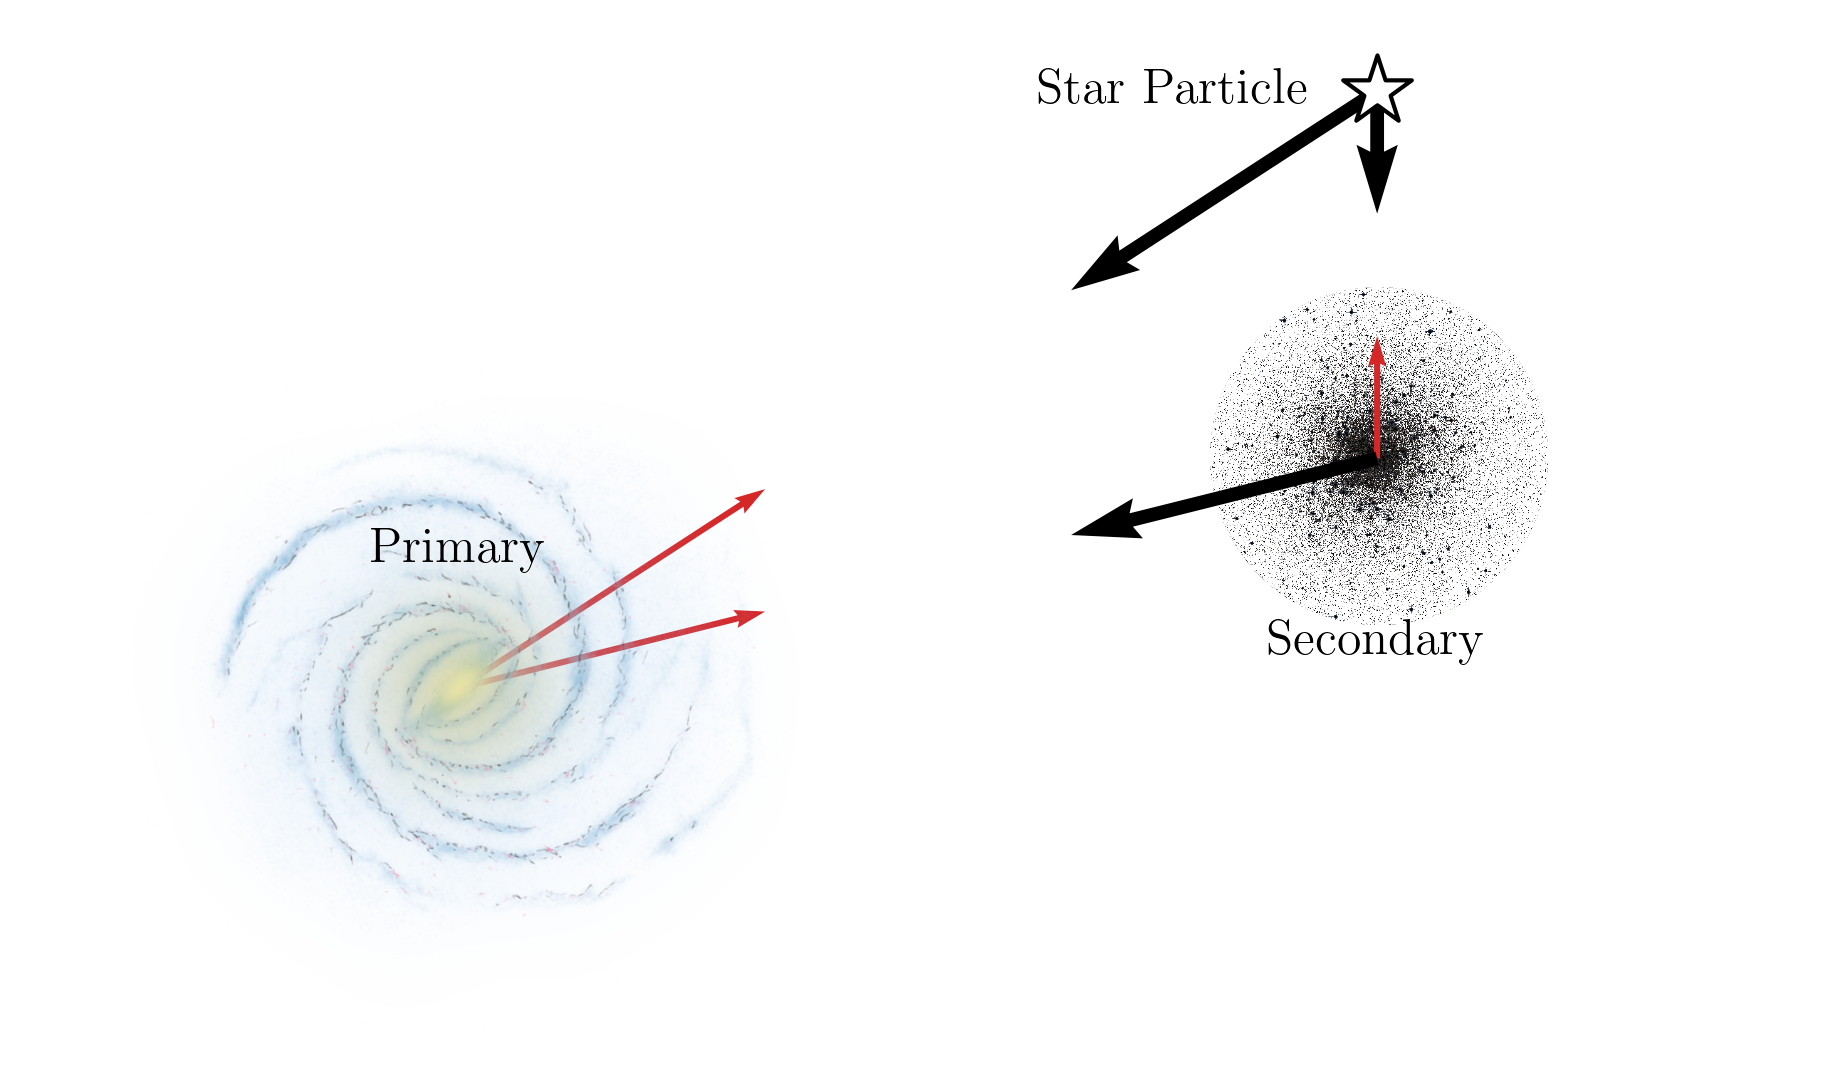
\includegraphics[width=.8\linewidth]{images/restricted_three_body_set_up.png}
        \caption[Schematic illustration of the restricted three-body setup]{Schematic illustration of the restricted three-body setup. The system is reduced to three interacting components: the Galaxy (primary), the globular cluster (secondary), and a single star (tertiary). Red vectors indicate forces that are neglected, while the black vectors are those that we model.}
        \label{fig:restricted_three_body_set_up}
    \end{figure}
    This formulation dramatically simplifies the dynamics: the full $N$-body problem is approximated by \(N\) independent realizations of the restricted three-body problem. This reduction allows us to efficiently simulate the formation and evolution of tidal features without incurring the computational cost of tracking all mutual interactions among stars. This approximation has been shown to work very well for certain stellar streams and this thesis is not the first time such methods have been employed. For instance, consider the work of \citet{2012A&A...546L...7M}, who modeled the evolution of the Palomar~5's stellar stream with both an $N$-body code as well as the restricted~three body problem. The differences between the two models for reproducing many characteristics of the stream are minimal. 

    In the remainder of this section, I present the theoretical framework underlying the simulations. At their core, the simulations involve solving \(N\) sets of six coupled ordinary differential equations -- one set for each star particle. Section~\ref{subsec:myEquationsOfMotion} introduces the equations of motion. Section~\ref{subsec:gravfield} describes the gravitational field used to compute the forces acting on the particles. Finally, Section~\ref{subsec:initialconditions} details the procedure used to generate initial conditions that faithfully represent a globular cluster.
    \subsection{Equations of Motion} \label{subsec:myEquationsOfMotion}
        In galactic dynamics, we can well describe the motion of stars through Poisson's equation, which extends Newton's law of gravity from point masses to smooth density distributions: 
        \begin{equation} \label{eq:poissonsequation}
            \nabla^2 \Phi = 4\pi G \rho,
        \end{equation}
        where $\rho$ is the mass density and $\Phi$ is the gravitational potential. We use Newtonian mechanics throughout this work because $\Phi << c^2$ in all relevant regimes, meaning General Relativity is not required \citep[see Appendix C of][]{bovy_inprep}. Poisson's equation assumes Newton's postulate that gravitational forces act instantaneously and that masses attract each other along the line connecting them. \footnote{Galaxies span millions of light-years, so how can Newton's assumption of instantaneous gravity be valid, given that gravitational waves travel at the speed of light? As shown by \citet{2000PhLA..267...81C}, this is well understood in General Relativity: the gravitational field encodes not only the position but also the motion of massive bodies. This ensures that the resulting spacetime curvature produces a force equivalent to attraction toward the body's instantaneous position, rather than where it was when the gravitational influence was emitted.}

        Instead of writing down the gravitational forces through Newton's second law, I will write down Hamilton's equations derived from the variational principle of Lagrangian mechanics. The full interacting system includes the kinetic energy of the globular cluster and the star particle, as well as three gravitational potential energy terms: the cluster-galaxy interaction, the particle-galaxy interaction, and the particle-cluster interaction:
        \begin{equation}
            \mathcal{L} = \frac{1}{2} M_{\rm gc} \dot{\mathbf{R}}_{\rm gc}^2 
                        + \frac{1}{2} m \dot{\mathbf{r}}^2 
                        - M_{\rm gc} \Phi_{\rm gal}(\mathbf{R}_{\rm gc}) 
                        - m \Phi_{\rm gal}(\mathbf{r}) 
                        - m \Phi_{\rm gc}(\mathbf{r} - \mathbf{R}_{\rm gc}).
        \end{equation}  
        $M_{\mathrm{gc}}$ is the mass of the globular cluster, $m$ is the mass of a star, $\mathbf{R}_{\mathrm{gc}}$ is the galacto-centric position of the globular cluster, $r$ is the galacto-centric position of the star, $\Phi_{\rm gal}$ is the potential generated by the galaxy and $\Phi_{\mathrm{gc}}$ is the potential generated by the globular cluster. We decouple the equations of motion of the globular cluster and the star. The justification for this approximation is evident when we normalize the Lagrangian by the cluster mass. This yields:
        \begin{equation}
            \frac{\mathcal{L}}{M_{\rm gc}} = \frac{1}{2} \dot{\mathbf{R}}_{\rm gc}^2 
                                        - \Phi_{\rm gal}(\mathbf{R}_{\rm gc}) 
                                        + \underbrace{\frac{m}{M_{\rm gc}} \left[ \frac{1}{2} \dot{\mathbf{r}}^2 
                                        - \Phi_{\rm gal}(\mathbf{r}) 
                                        - \Phi_{\rm gc}(\mathbf{r} - \mathbf{R}_{\rm gc}) \right]}_{\text{negligible correction to GC's motion}}
        \end{equation}
        In the limit where \( m << M_{\rm gc} \), the terms in brackets become negligible, and the star's motion has no influence on the cluster. The Lagrangian for the cluster's orbit thus becomes:
        \begin{equation}
            \frac{\mathcal{L}_{\mathrm{gc}}}{M_{\mathrm{gc}}} = \frac{1}{2} \dot{\mathbf{R}}_{\rm gc}^2 
                                - \Phi_{\rm gal}(\mathbf{R}_{\rm gc})
        \end{equation}
        Switching to the star's perspective, we normalize the Lagrangian by the particle mass \( m \), obtaining:
        \begin{equation}\label{eq:starParticleLagrangian}
            \frac{\mathcal{L}_{\rm star}}{m} = \frac{1}{2} \dot{\mathbf{r}}^2 
                                - \Phi_{\rm gal}(\mathbf{r}) 
                                - \Phi_{\rm gc}(\mathbf{r} - \mathbf{R}_{\rm gc}(t))
        \end{equation}
        Here, the cluster's influence on the particle is retained through its time-dependent position \( \mathbf{R}_{\rm gc}(t) \). This influence becomes important when the gravitational forces from the cluster and the galaxy on the particle are comparable. For a quick estimate, we can treat both the galaxy and the cluster as point masses. The two forces become comparable when the particle is sufficiently close to the cluster, which occurs when: $|\mathbf{r} - \mathbf{R}_\mathrm{GC}| < \sqrt{\frac{M_{\mathrm{gc}}}{M_{\mathrm{ gal}}}} |\mathbf{r}|.$ In other words, the cluster's gravitational field dominates over the galaxy's on sufficiently small scales around the cluster -- as expected. For a quick sanity check: a typical globular cluster may have a mass of \(10^5\, M_\odot\), while the Milky Way may be around \(10^{12}\, M_\odot\) \citep{2025NewAR.10001721H}. If the cluster is a few kiloparsecs from the galactic center, then the cluster's influence dominates within a region of order a few parsecs -- which checks out. A better limit is the tidal radius and is presented in the next section.

        Next, working in the Hamiltonian formalism often provides deeper insight into the physics of the system. Additionally, Hamiltonian mechanics reduces the equations of motion to a set of \(2N\) first-order differential equations, rather than \(N\) second-order ones, which is more convenient for computational integration.

        The Hamiltonian can then be obtained via a Legendre transform: \(\mathcal{H} = \sum p_i \dot{q}_i - \mathcal{L},\) where $q$ is a generic position coordinate, $p$ is its conjugate momentum, while $i$ indicates the coordinate of interest. If we use the \textit{specific} Lagrangian -- normalized by the mass of the body of interest -- then, in Cartesian coordinates, the conjugate momenta reduce to the velocities: $p_i=\frac{\partial \mathcal{L}}{\partial q} \rightarrow p_i = v_i$. Another useful result comes from Noether's theorem: if a coordinate does not explicitly appear in the Lagrangian, its conjugate momentum is conserved. Most of the galactic potentials considered in our simulation are axis-symmetric meaning they have cylindrical symmetry, except for case of a rotating stellar bar. Since the Lagrangian does not depend on the azimuthal angle \( \theta \) in the \(x\text{-}y\) plane for the cluster's motion, the \(z\)-component of angular momentum is conserved: $p_\theta = L_z = \frac{\partial \mathcal{L}}{\partial \dot{\theta}} = R^2 \dot{\theta} = \mathrm{constant.}$

        If we consider a star within an isolated globular cluster with spherical symmetry, its total angular momentum vector is conserved. However, if we consider the Eq.~\ref{eq:starParticleLagrangian}, then no quantities are conserved. There are no symmetries, and due to the explicit time dependence, energy is not conserved either. On the other hand, if a star-particle is sufficiently far from the globular cluster, such that its motion is governed solely by the galactic potential, then conservation of $L_z$ is recovered in the case of an axisymmetric Galactic potential.

        Hamilton's equations thus provide the time evolution of the momenta and the positions. In Cartesian coordinates, the equations of motion for the cluster are: 
        \begin{equation}\label{eq:equations_of_motion_cluster}
            \begin{aligned}
                \dot{p}_{x,\mathrm{gc}} &= -\frac{\partial \Phi_\mathrm{gal}\left(\mathbf{R}_{\mathrm{gc}}\right)}{\partial x} \\
                \dot{p}_{y,\mathrm{gc}} &= -\frac{\partial \Phi_\mathrm{gal}\left(\mathbf{R}_{\mathrm{gc}}\right)}{\partial y} \\
                \dot{p}_{z,\mathrm{gc}} &= -\frac{\partial \Phi_\mathrm{gal}\left(\mathbf{R}_{\mathrm{gc}}\right)}{\partial z} \\
                \dot{x}_{\mathrm{gc}} &= p_{\mathrm{gc},x} \\
                \dot{y}_{\mathrm{gc}} &= p_{\mathrm{gc},y} \\
                \dot{z}_{\mathrm{gc}} &= p_{\mathrm{gc},z}.
            \end{aligned}
        \end{equation}
        For the star particle, the equations of motion become: 
        \begin{equation}\label{eq:equations_of_motion_stream}
            \begin{aligned}
                \dot{p}_{x} &= -\frac{\partial \Phi_\mathrm{gal}\left(\mathbf{r}\right)}{\partial x} - \frac{\partial \Phi_\mathrm{gc}\left(\mathbf{r} - \mathbf{R}_{\mathrm{gc}}(t)\right)}{\partial x}\\
                \dot{p}_{y} &= -\frac{\partial \Phi_\mathrm{gal}\left(\mathbf{r}\right)}{\partial y} - \frac{\partial \Phi_\mathrm{gc}\left(\mathbf{r} - \mathbf{R}_{\mathrm{gc}}(t)\right)}{\partial y}\\
                \dot{p}_{z} &= -\frac{\partial \Phi_\mathrm{gal}\left(\mathbf{r}\right)}{\partial z} - \frac{\partial \Phi_\mathrm{gc}\left(\mathbf{r} - \mathbf{R}_{\mathrm{gc}}(t)\right)}{\partial z}\\
                \dot{x} &= p_x \\
                \dot{y} &= p_y \\
                \dot{z} &= p_z,
            \end{aligned}
        \end{equation} 
        Note that equation~\ref{eq:equations_of_motion_stream} describes the motion of a single particle. In general, if we use 100,000 particles, the motion of each is described with this same equation, but has different initial conditions. 
        
        Equation~\ref{eq:equations_of_motion_cluster} describes the motion of a globular cluster within the Galactic potential, while Equation~\ref{eq:equations_of_motion_stream} models the evolution of stars within the cluster and the formation of a stellar stream, assuming a fixed orbital path for the cluster. However, globular clusters do not evolve in isolation. To explore interactions, such as those between clusters and nearby streams, we must extend the equations of motion accordingly. This is the central focus of Chapter~5, which investigates how globular clusters can perturb neighboring stellar streams.

        To capture such interactions, we first modify Equation~\ref{eq:equations_of_motion_cluster} to include mutual gravitational forces between all clusters, effectively computing $N$-body interactions among them. While full $N$-body dynamics are typically avoided due to computational cost, this extension is tractable here, as the system includes only about 160 clusters. The resulting modified equations are:
        \begin{equation}\label{eq:equations_of_motion_cluster_n_body}
            \begin{aligned}
                \dot{p}_{x,i} = - \frac{\partial \Phi_\mathrm{gal}}{\partial x} - \sum_{j\neq i}^N \left[\frac{\partial \Phi_\mathrm{gc}\left(\mathbf{R}_i-\mathbf{R}_j|M_j,b_j\right)}{\partial x}\right], \\ 
                \dot{p}_{y,i} = - \frac{\partial \Phi_\mathrm{gal}}{\partial y} - \sum_{j\neq i}^N \left[\frac{\partial \Phi_\mathrm{gc}\left(\mathbf{R}_i-\mathbf{R}_j|M_j,b_j\right)}{\partial y}\right], \\ 
                \dot{p}_{z,i} = - \frac{\partial \Phi_\mathrm{gal}}{\partial z} - \sum_{j\neq i}^N \left[\frac{\partial \Phi_\mathrm{gc}\left(\mathbf{R}_i-\mathbf{R}_j|M_j,b_j\right)}{\partial z}\right],
            \end{aligned}
        \end{equation}
        where $i$ is the index of a target cluster and $j$ iterates over the others. Note that in $\Phi_{\mathrm{gc}}$, I explicitly write $M_j,b_j$ to indicate the mass and scale length of the $j^{\mathrm{th}}$ cluster. Each cluster has its own scale-length, which were computed from the half-mass radii reported in \citet{2018MNRAS.478.1520B}. Since each cluster is modeled with a distinct scale radius, Newton's third law is not strictly satisfied: $\dot{\mathbf{p}}_{ij} \neq -\dot{\mathbf{p}}_{ji}$\footnote{We define the force exerted by cluster $j$ on cluster $i$ as $\mathbf{p}_{ij} = \frac{-G M_i M_j}{\left(b_j^2 + r_{ij}^2\right)^{3/2}} \mathbf{r}_{ij}$, where $\mathbf{r}_{ij} = \mathbf{r}_i - \mathbf{r}_j$ and $b_j$ is the Plummer scale radius of cluster $j$. When $b_i \neq b_j$, the forces are not equal and opposite, thus violating Newton's third law. However, in the limit $r_{ij} \gg b_i, b_j$, this asymmetry vanishes, and the interaction reduces to that of point masses.}. This violation is not dynamically significant in practice. Since each cluster is modeled as a Plummer sphere, the force profile converges to that of a point mass at distances much greater than the scale radius. As a result, the approximation remains valid for most inter-cluster separations.

        Lastly, in terms of the stream generation for Chapter~5, equation~\ref{eq:equations_of_motion_stream} are also modified to include the force from all the clusters, instead of just the host cluster. This becomes: 
        \begin{equation}
            \begin{aligned}
                \dot{p}_{x} &= -\frac{\partial \Phi_\mathrm{gal}\left(\mathbf{r}\right)}{\partial x} - \sum_i^N \frac{\partial \Phi_\mathrm{gc}\left(\mathbf{r} - \mathbf{R}_i(t)\right)}{\partial x}\\
                \dot{p}_{y} &= -\frac{\partial \Phi_\mathrm{gal}\left(\mathbf{r}\right)}{\partial y} - \sum_i^N \frac{\partial \Phi_\mathrm{gc}\left(\mathbf{r} - \mathbf{R}_i(t)\right)}{\partial y}\\
                \dot{p}_{z} &= -\frac{\partial \Phi_\mathrm{gal}\left(\mathbf{r}\right)}{\partial z} - \sum_i^N \frac{\partial \Phi_\mathrm{gc}\left(\mathbf{r} - \mathbf{R}_i(t)\right)}{\partial z}
            \end{aligned}
        \end{equation}
        The first two sets of equations are used to model the streams associated with each of the Galactic globular clusters, in a system where each cluster is subject only to the gravitational pull of the Galaxy. The second set of equations takes into account the fact that each cluster, and each particle in its stream, is generally also influenced by the gravitational pull of all the other Galactic globular clusters. The next two subsections introduce the various forms that $\Phi$ can take, followed by the generation of the initial conditions. 

    \subsection{The Gravitational Field} \label{subsec:gravfield}
        Determining the gravitational field of the Milky Way remains an open and complex problem. From our location within the Galaxy, it is difficult to obtain a global perspective. Since the advent of extragalactic astronomy and early classification efforts such as those by \citet{1926ApJ....64..321H}, we have begun to ask what the total structure of our own Galaxy is. Before providing a robust estimate for the global mass distribution, some simpler questions were addressed. For example, \citet{1927BAN.....4...91O} studied the motion of stars in the local solar neighborhood and showed that the Galaxy not only has net rotation, but also differential rotation -- as opposed to solid-body rotation.

        The field has come a long way since then, and today we possess a number of viable models for the Galactic gravitational field. Much of our understanding owes to the fact that Poisson's equation is linear:
        \begin{equation}\label{eq:linear_poisson}
            \nabla^2 \left(a_0\Phi_0 + a_1\Phi_1 \right) = a_0 \nabla^2 \Phi_0 + a_1 \nabla^2 \Phi_1 = 4\pi G \left(a_0\rho_0 +a_1\rho_1\right),
        \end{equation}
        which allows us to treat the Galaxy as a superposition of separate components, each described by its own potential-density pair. This decomposition enables the construction of composite models from a collection of structural elements that are also commonly observed in external galaxies. The Galaxy Zoo project \citep{2008MNRAS.389.1179L}, for instance, has shown that many galaxies share similar morphologies, justifying this modular approach. The Milky Way is no exception. Typical components of disc like galaxies are:
        \begin{itemize}
            \item A stellar disk,
            \item A gaseous disk,
            \item A dark matter halo,
            \item A stellar halo,
            \item A bulge,
            \item A galactic bar,
            \item Spiral arms.
        \end{itemize}
        In addition, smaller-scale structures such as globular clusters, giant molecular clouds, and open clusters can locally perturb the field. Even external sources, such as the Large and Small Magellanic Clouds, play a role by inducing measurable tidal effects on the Galaxy \citep[see, for example][]{2021MNRAS.501.2279V,2022ApJ...939....2A}.

        Despite this framework, modeling remains difficult because the structural components are not isolated. As emphasized by \citet{2016ARA&A..54..529B}, the components co-evolve within a shared potential, meaning that even those formed separately eventually become dynamically mixed. This interdependence implies that the potential cannot be cleanly partitioned into independent contributions, and even with a complete dataset, degeneracies would persist. Their review illustrates this point by listing 37 parameter groups required to characterize the Galaxy -- including the local standard of rest, Galactic reference frame, and the geometric and density properties of various components -- underscoring the system's complexity.

        The challenge is compounded by limitations in the available data. The Gaia mission has delivered the most comprehensive survey of the Galaxy to date \citep{2023A&A...674A...1G}, providing photometric and astrometric data for over two billion stars and radial velocities for tens of millions \citep{2018A&A...616A..11G}. However, this still represents only a small fraction of the total stellar population. The stellar mass of the Milky Way is estimated to be approximately $6\times10^{10} \mathrm{M}_\odot$ \citep{2015ApJ...806...96L}, corresponding to roughly one hundred billion stars \citep[see also][]{2017MNRAS.465...76M}. Thus, Gaia provides 5D phase-space information for only about 1-2\% of all stars, and full 6D information for just a fraction of a percent.

        Moreover, the data suffer from unavoidable selection effects. As illustrated in Fig.~\ref{fig:gaia_selection_function}, which shows the spatial distribution of stars with spectroscopic observations from Gaia DR3, the bulk of high-quality measurements are clustered near the Sun. This is a natural consequence of the inverse-square law for luminosity, and it implies that any model of the Galactic potential must account for these biases \citep{2025A&A...695A.220K}.
        \begin{figure}
            \includegraphics[width=\linewidth]{images/recio-blanco-2023-fig5}
            \caption[The spatial distribution of stars with spectroscopic measurements in Gaia DR3]{The spatial distribution of stars with spectroscopic measurements in Gaia DR3. Figure 5 from \citet{2023A&A...674A..38G}.}
            \label{fig:gaia_selection_function}
        \end{figure}
        In summary, while we now possess sophisticated models and rich datasets, constructing a comprehensive and precise model of the Milky Way's gravitational field is still inherently difficult -- constrained both by observational incompleteness and the physical complexity of a system in which all components are tightly coupled. Given these challenges, the construction of a Galactic model depends on the scientific question being asked.

        Consider \texttt{TRILEGAL} \citep{2005A&A...436..895G}. This model aims to answer the question: if I observe the sky from a given location with a given instrument, what do I expect to see? The focus of these models are stellar populations. Dynamics—such as orbits or gravitational forces—are secondary and not included in the construction. The primary goal is to reproduce observed star counts and understand the underlying stellar populations. Such models are designed to simulate the sky as it would appear to missions like Hipparcos \citep{1997A&A...323L..49P}, 2MASS \citep{2006AJ....131.1163S}, and SDSS \citep{2000AJ....120.1579Y}.

        Some models attempt to address both stellar populations and dynamics. For example, the Besançon model aims to construct a dynamically self-consistent model of the Milky Way that reproduces observables such as the rotation curve, as well as the spatial and chemical distributions of stars. The model originated with \citet{1986A&A...157...71R, 1987A&A...180...94B}, and was eventually improved with Hipparcos data \citep{2003A&A...409..523R}. The authors decomposed the galaxy into a thin disk, a thick disk, a stellar halo, and a bulge, with each component assigned its own star formation rate and initial mass function. The model has been continuously refined; for instance, \citet{2022A&A...667A..98R} incorporated Gaia DR3 kinematics to further constrain it. As noted by \citet{2025AJ....169..317K}, who recently introduced the open-source Python package \texttt{SYNTHPOP} for simulating on-sky photometry, the success of TRILEGAL and the Besançon model lies in their openness: they are publicly available and have web interfaces for widespread use. These tools are particularly valuable for creating mock surveys of the sky.

        A different approach is taken by \citet{2024MNRAS.527.1915B}, building on \citet{2023MNRAS.520.1832B}, who constructed a dynamical model of the Milky Way in which the distribution function depends on orbital actions—quantities that are conserved along orbits in a steady-state potential. In axisymmetric potentials, the actions are $J_r$, $J_\phi$, and $J_z$, and represent how much motion an orbit has in the radial, azimuthal, and vertical directions, respectively. The moments of the distribution function yield observable quantities such as stellar surface densities, volume densities, and velocity dispersions. In addition to dynamical consistency, the model includes the chemical properties of stars, specifically metallicity ([Fe/H]) and $\alpha$-element abundances. The model is constrained using Gaia DR3 data \citep{2023A&A...674A...1G}, particularly stars with full phase-space information, as well as APOGEE DR17 \citep{2017AJ....154...94M}. Their model involves over 40 parameters to describe the distributions of stars and metallicities throughout the Milky Way.

        Then, there are many models of the Milky Way that are primarily dynamically motivated, with stellar populations treated as secondary \citep[see, for example,][]{1991RMxAA..22..255A,2015ApJS..216...29B,2017MNRAS.465...76M,2017A&A...598A..66P,2024ApJ...967...89I}. Despite the variety, their construction generally follows the same template: the authors must select a dataset, tracer populations, and the parametric form of the Milky Way potential. Often, fitting all model parameters is infeasible, whether due to lack of data, high computational cost, or non-converging likelihoods. Thus, the authors will assume fixed values for some parameters. 

        All of the above models assume axisymmetry, which is already a limitation. This makes it difficult to model the dynamics in the inner Galaxy (within a few~$\mathrm{kpc}$). Both \citet{2017MNRAS.465...76M} and \citet{2024MNRAS.527.1915B} fix the parameters describing the gas in the Galactic disk and only fit those related to the stellar and dark matter distributions. \citet{2017MNRAS.465...76M} specifically constructed their model to support orbit calculations for stars in anticipation of Gaia data releases. They aimed to improve upon their earlier model \citep{2011MNRAS.414.2446M}, motivated by (1) a tripling of the maser population used to trace disk kinematics, and (2) the realization that omitting a gaseous disk in their earlier work had led to underestimating the forces in the solar vicinity.

        Many of the models described above rely on fitting data using kinematic information, comparing the model's predictions for velocity dispersion to observations of large samples of stars. This is because direct astrometric measurements of stellar accelerations are still in their infancy. Measuring changes in angular position through parallax is so challenging that stars were long referred to as \textit{fixed stars} \citep{1981unht.book.....K}. Precise, year-over-year positional measurements are required to observe motion on the celestial sphere, precisely what Gaia does.

        That said, accelerations have been measured in some cases. \citet{2018ApJS..239...31B,2021ApJS..254...42B} created a cross-catalog between Hipparcos and Gaia DR2 \citep{2018A&A...616A...1G} and later EDR3. This provided a baseline of over 25 years, long enough to detect accelerations for some stars. However, the Hipparcos catalog only contains around 100,000 stars, and the typical acceleration of a field star in the Galaxy is extremely small. Consequently, the cross-matched catalog is currently being used to study stars with unusually high accelerations. These stars are typically in binary systems or have massive planets \citep{2023MNRAS.521.5232W,2025AJ....170...52G}, and their detectable accelerations are not due to the Galactic gravitational field.

        As stated in the motivation for undertaking this thesis, stellar streams are particularly useful for recovering information about the Galactic gravitational field. The stars within a stream are on similar orbits (but shifted in phase), and their orientation and curvature encodes detailed information about the Galactic gravitational field. \citet{2024ApJ...967...89I} is the first study to use an ensemble of stellar streams to directly fit a gravitational potential model of the Milky Way \citep[see also][who also used streams to infer Galactic potential parameters]{2010AAS...21532103L,2016ApJ...833...31B}. Even in that case, \citet{2024ApJ...967...89I} needed to fix some of the model parameters. For example, they adopted the same bulge model as \citet{2017MNRAS.465...76M}.

        In this thesis, we use the models of \citet{2017A&A...598A..66P}, which build upon the work of \citet{1991RMxAA..22..255A}. These models were developed within our research group and were available at the start of the project. They were designed to fit observational data similar to those used in \citet{2015ApJS..216...29B}, including the Galactic rotation curve and local stellar kinematics. \citet{2017A&A...598A..66P} were motivated to create a new Galactic model that included a thick disk \citep{1983MNRAS.202.1025G} since \citet{2013A&A...560A.109H} and \citet{2015A&A...578A..87S} demonstrated that the thick disk has comparable mass to the thin disk. \citet{2017A&A...598A..66P} thus provide two Milky Way potential models: one with a bulge and one without. Below, we describe the second version, which is used in both Chapter~4 and Chapter~5.

        An excellent quality of the models presented \citet{2017A&A...598A..66P} is that they are fully analytic. The first model comprises two disks, a bulge, and a halo, while the second model omits the bulge. The disk are modeled with the Miyamoto-Nagai potential \citep{1975PASJ...27..533M}:
        \begin{equation}
            \Phi(R, z \mid M, a, b) = -\frac{G M}{\sqrt{R^2 + \left(a + \sqrt{z^2 + b^2}\right)^2}},
        \end{equation}
        where $M$ is the total mass of the disk, $a$ is the radial scale length, and $b$ is the vertical scale height. This form smoothly interpolates between a flattened disk and a spherical distribution, depending on the values of $a$ and $b$. \citet{2015ApJS..216...29B} also used this form for their disk model.

        However, it is worth noting that galactic disks can have more complicated functional forms. For instance, \citet{1970ApJ...160..811F} noticed that stellar densities in disks generally decay exponentially:
        \begin{equation}\label{eq:exponentialDisk}
            \rho(R,z) = \rho_0 \mathrm{exp}\left(-\frac{R}{R_d}-\frac{|z|}{z_d}\right),
        \end{equation}
        where $\rho$ is the mass density, $R$ is the cylindrical radius, $z$ the vertical height, and the model has three parameters: a characteristic density $\rho_0$, scale radius $R_d$, and scale height $z_d$. \citet{2006A&A...454..759P} continued this analysis and showed that a single exponential often cannot capture the true decay, and in many galaxies there is a transition radius where the profile can significantly change. A drawback of this model in equation~\ref{eq:exponentialDisk} is that it cannot be integrated analytically to obtain the potential, since the $R$ and $z$ coordinates are not separable. Often, basis function expansions are needed to approximate the potential and compute forces. \citet{2017MNRAS.465...76M} and \citet{2024ApJ...967...89I} both adopted this model for their Galactic disks.

        Regarding the halo, \citet{2017A&A...598A..66P} use a single halo model to represent both the stellar and dark matter contributions, since the stellar mass contribution is negligible; \citet{2022A&A...667A..98R} estimate the stellar halo mass to be $3.17 \times 10^8~\mathrm{M}_\odot$. The halo model is inherited from \citet{1991RMxAA..22..255A}, originally proposed in \citet{1986RMxAA..13..137A}. It is designed so that beyond a certain scale radius, the enclosed mass grows linearly with distance, leading to the desirable feature of a flat rotation curve:
        \begin{equation} 
            M_{\mathrm{enc}}(r|M_0,\gamma,r_0,r_c) = M_0
            \begin{cases}
             \frac{\left(r/r_0\right)^\gamma}{1 + \left(r/r_0\right)^{\gamma - 1}} & r<r_c,\\
             \frac{\left(r_c/r_0\right)^\gamma}{1 + \left(r_c/r_0\right)^{\gamma - 1}} & r> r_c,\\
            \end{cases} 
            \label{eq:martos_enclosed_mass}
        \end{equation}
        where $M_0$ is a mass scaling parameter (not the total mass), $r_0$ is the characteristic radius, $\gamma$ is the power-law index, and $r_c$ is a cutoff radius beyond which the mass is held constant. Thus, for $r > r_c$, Eq.~\ref{eq:martos_enclosed_mass} yields the total mass. 

        In the outer regime $(r/r_0) >> 1$, the enclosed mass scales as $M(r) \propto r$, producing a flat rotation curve. In the inner regime $(r/r_0) << 1$, the mass grows as a power law, $M(r) \propto r^{\gamma - 1}$, which provides flexibility in shaping the central density slope. Since the unmodified profile leads to an nonphysical divergence in total mass, a truncation at $r_c$ is imposed.

        Given spherical symmetry, we may use the relation $\nabla \Phi = \frac{G M_{\mathrm{enc}}(r)}{r^2}$. Requiring that the potential vanish at infinity, the corresponding gravitational potential can be obtained by integrating:
        \begin{equation}
            \Phi(r|M_0,\gamma,r_0,r_c) = 
            \begin{cases}
                \frac{GM_0}{r_0\left(\gamma-1\right)}\ln\left|\frac{1+(r/r_0)^{\gamma-1}}{1+(r_c/r_0)^{\gamma-1}}\right| -\frac{GM_t}{r_c}, & r<r_c\\
                -\frac{GM_t}{r} & r>r_c.
            \end{cases}
        \end{equation}
        where $M_t$ denotes the total mass, $M_{\mathrm{enc}}(r_c)$. In general, a good halo model should reproduce the observed flat rotation curve at large radii. Another class of models that achieves this are the double power-law profiles:
        \begin{equation}
            \rho(r \mid \alpha, \beta, r_s) = \rho_0 \left( \frac{r}{r_s} \right)^{-\alpha} \left(1 + \frac{r}{r_s} \right)^{\alpha - \beta},
        \end{equation}
        where $r_s$ is a scale radius, $\alpha$ controls the inner slope, and $\beta$ the outer slope. Common choices include the NFW profile ($\alpha = 1$, $\beta = 3$) and the Hernquist profile ($\alpha = 1$, $\beta = 4$). These families of models were implemented in the works of \citet{2015ApJS..216...29B, 2017MNRAS.465...76M} to describe the dark matter halo.

        The two disks and the halo constitute the second model of \citet{2017A&A...598A..66P}. I present this in Fig.~\ref{fig:figure_pouliasis2017pii_potential}, as it was employed in both studies. See their paper for more visualizations of the potential and the version that includes a bulge.
        \begin{figure}
            \centering
            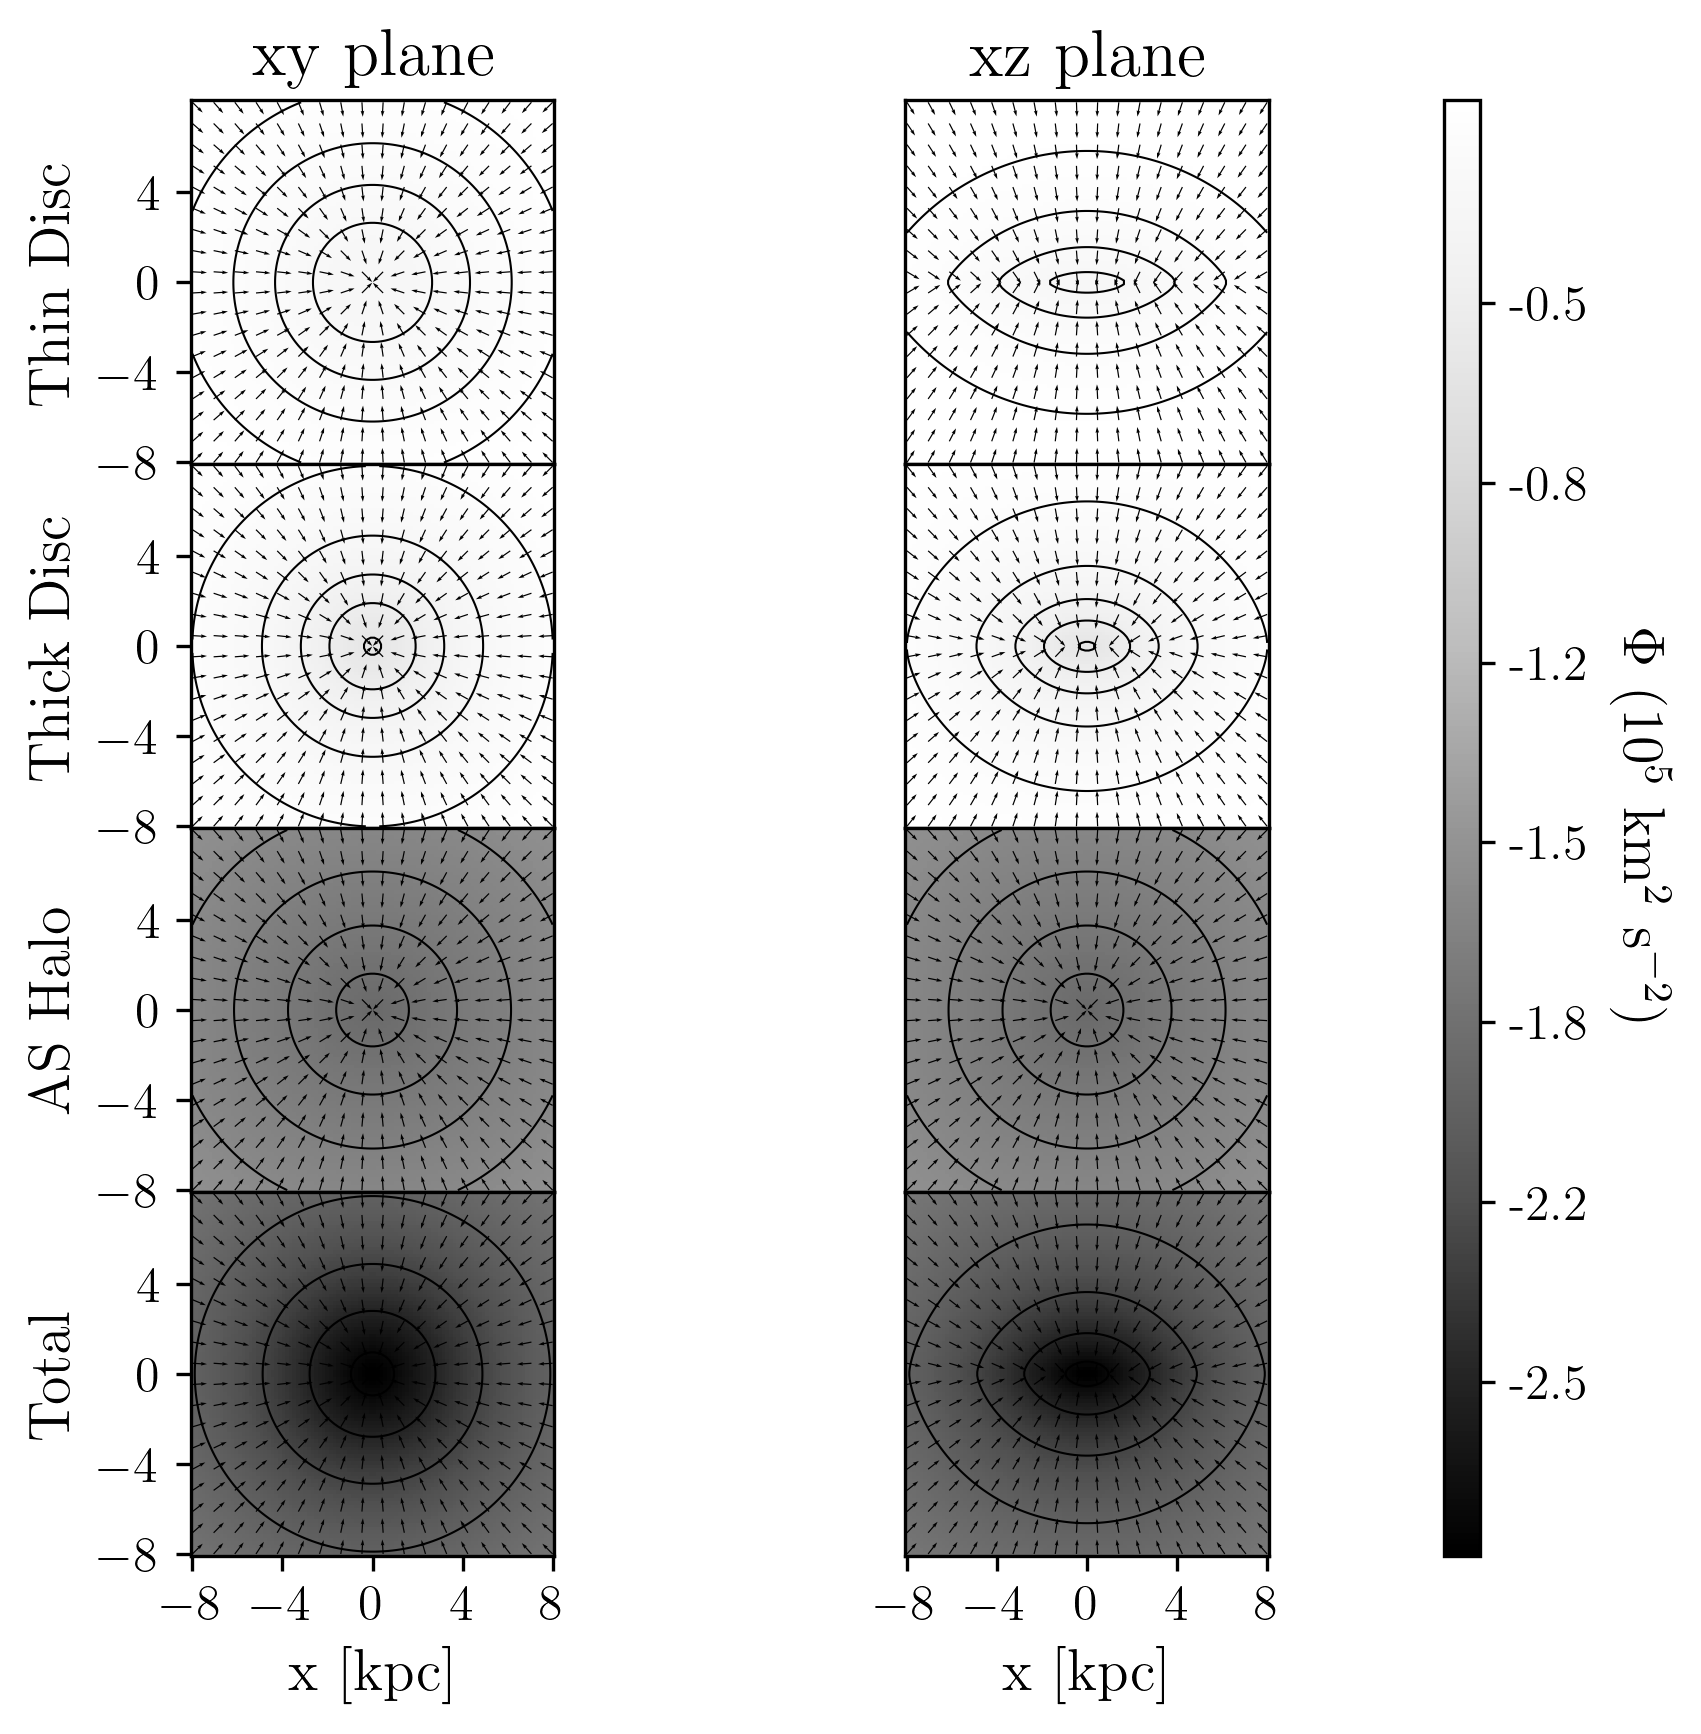
\includegraphics[width=\linewidth]{images/figure_pouliasis2017pii_potential_-8_8.png}
            \caption[Gravitational field from \citet{2017A&A...598A..66P}]{Individual components of the second Galactic potential model from \citet{2017A&A...598A..66P}. The vector field illustrates the normalized gravitational force at each position, corresponding to $\vec{g} = -\nabla\Phi$. Equipotential contour lines are overlaid to guide the eye.}
            \label{fig:figure_pouliasis2017pii_potential}
        \end{figure}
        
        In Chapters~4 and~6 (preliminary results), we model the inner Galaxy using the triaxial bar potential of \citet{1992ApJ...397...44L}. The model is constructed by representing the bar as a uniform-density ``needle'' aligned with the $x$-axis and convolving it with a Miyamoto-Nagai disk flattened along the $z$-axis. The resulting potential is: 
        \begin{equation}
            \Phi(x,y,z\,|\,M,a,b,c) = \frac{GM}{2a} \ln\left( \frac{x-a+T_{-}}{x+a+T_{+}} \right),
        \end{equation}
        with
        \begin{equation}
            T_{\pm} = \left[ (a \pm x)^2 + y^2 + \left( b + \sqrt{c^2 + z^2} \right)^2 \right]^{1/2}.
        \end{equation}
        Here $M$ is the total mass of the bar, $a$ is the semi-major axis, and $b$ and $c$ are the intermediate- and short-axis scales, respectively. The axis ratio $c/b$ controls the vertical thickness: $c/b \to \infty$ corresponds to a prolate bar, while $c/b \to 0$ yields a flat, planar bar.

        While the bar can account for much of the inner Galaxy's mass distribution, some models include an additional, centrally concentrated component conventionally referred to as the \emph{bulge}. In the mass model of \citet{2017A&A...598A..66P}, the bulge is represented by a Plummer sphere \citep{1911MNRAS..71..460P}, an analytic potential with two parameters—the total mass and a scale length—given by
        \begin{equation} \label{eq:plummer}
            \Phi(r \mid M, b) = -\frac{G M}{\sqrt{r^2 + b^2}},
        \end{equation}
        where $M$ is the total mass and $b$ is the scale length. In the limit $a \rightarrow 0$, the Miyamoto-Nagai potential reduces to the Plummer form. The Plummer sphere has a finite central potential, asymptotically approaches the potential of a point mass for $r >> b$, and produces a density profile that falls off as $\rho \propto r^{-5}$ at large radii. We also adopt the Plummer sphere as the analytic model for the globular clusters.

        How important is the choice of potential model when modeling the orbits of globular clusters? It depends on the specific cluster. Take, for instance, Fig.~\ref{fig:vasiliev_2021_EDR3_GCS_FIG_10}. The position and spread of some clusters are virtually identical between different models—for example, NGC~288. This suggests that the observational uncertainties in the kinematic data are larger than the discrepancies introduced by the choice of potential. However, for other clusters, the model choice has a much greater impact. A notable case is Pyxis, where the inferred orbits differ significantly depending on the potential. This effect is more pronounced for clusters located farther from the Galactic center, where the models diverge more strongly.
        \begin{figure}
            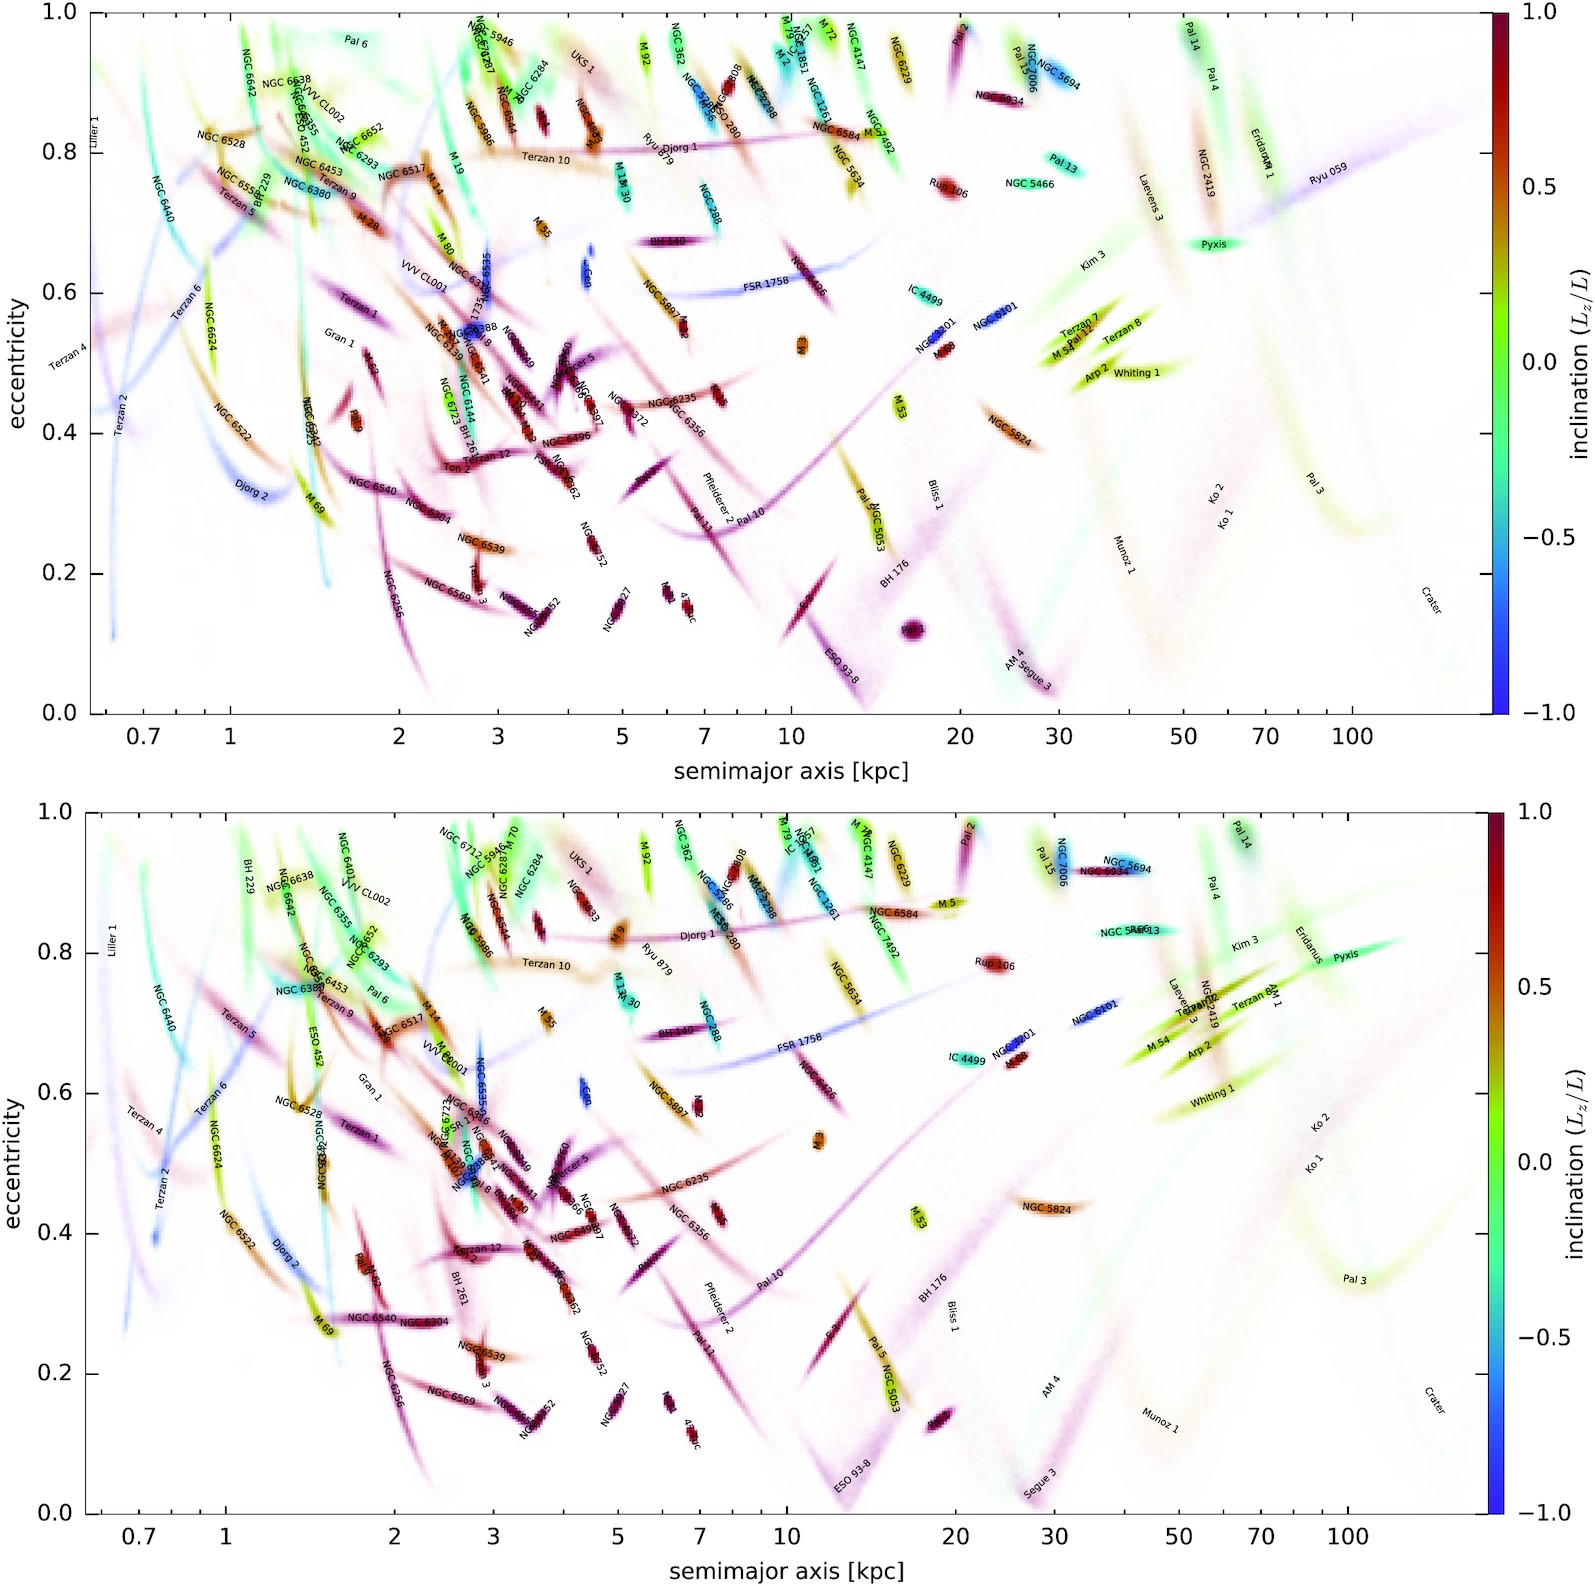
\includegraphics[width=\linewidth]{images/vasiliev_2021_EDR3_GCS_FIG_10.jpeg}
            \caption[Uncertainties in the Milky Way Globular Cluster orbital parameters]{Distribution of eccentricities, inclinations, and semi-major axes for the globular cluster population, based on Gaia EDR3 kinematics. Each point corresponds to a single realization of a globular cluster orbit, given its observational uncertainties. The top panel shows orbits computed using the potential from \citet{2017MNRAS.465...76M}, while the bottom panel uses the model from \citet{2015ApJS..216...29B}. (Credit: Fig.~10 from \citet{2021MNRAS.505.5978V})}
            \label{fig:vasiliev_2021_EDR3_GCS_FIG_10}
        \end{figure}
        Differences in cluster orbits-or in stellar streams evolved in different potentials-can help constrain the underlying Galactic potential and eventually lead to more accurate models of the Milky Way. This was the motivation behind recent work such as \citet{2024ApJ...967...89I}. However, if the goal is to make robust predictions or extrapolate properties of the halo, it is prudent to explore a variety of Galactic models, especially when no single model is clearly preferred.
    
    \subsection{Generating a Globular Cluster}\label{subsec:initialconditions}
        Now that the equations of motion established, and we have an accurate model for computing the gravitational force at each point in the Galaxy, what are the initial conditions? First, the initial conditions for the kinematics, mass, and size, of the globular clusters are taken observationally from \citet{2018MNRAS.478.1520B} \citep[this catalog was assembled across a series of works, see also][]{2017MNRAS.464.2174B,2019MNRAS.482.5138B,2020PASA...37...46B,2021MNRAS.505.5957B}\footnote{https://people.smp.uq.edu.au/HolgerBaumgardt/globular/}. Specifically, their estimated total masses, half-mass radii, as well as their on-sky ICRS coordinates, that we then convert to galacto-centric coordinates (see Chapters 4 and 5). What about initial conditions for the stars within the cluster? 

        We have chosen the gravitational potential of each cluster to follow a Plummer sphere, as given in Eq.~\ref{eq:plummer}. The corresponding mass profile can be sampled to generate initial positions for individual particles. However, positional information alone is insufficient, we must also assign appropriate velocities. One crude approach, following the sampling of positions, is to assign a velocity vector drawn isotropically; that is, with a direction uniformly distributed over the sphere. Furthermore, the speed could be sampled uniformly between zero and the local escape velocity. While this method can produce plausible initial conditions, it lacks \textit{self-consistency}, as the resulting phase-space distribution would not correspond to a stable equilibrium configuration of the chosen potential.

        In galactic dynamics, a fundamental challenge is the \textit{self-consistency problem}. This involves a loop of three steps:  
        \begin{enumerate}
            \item Given a density distribution and a gravitational potential (linked via Poisson's equation), one samples the positions of stars.  
            \item One then assigns initial velocities and evolves the system forward in time.  
            \item The potential is updated based on the evolved mass distribution.
        \end{enumerate}
        If the system is in equilibrium and self-consistent, then the mass distribution remains stable under its own gravity. That is, the same density that generated the potential continues to persist as the system evolves. For the rest of the section, I will describe in detail how one creates a self consistent system through the Collisionless Boltzmann Equation, and the simplifying assumptions employed in this thesis tackle our specific problem.

        Our starting point is to characterize the system statistically, with a distribution function (DF) over phase-space. That is, what is the probability density of finding a particle at a given position and velocity? This is encoded in the function \( f(\vec{x}, \vec{v}, t) \). If we treat this as a true probability density function that integrates to 1 over all phase space, we are implicitly assuming a closed system: no stars enter, leave, are born, or die.

        Already, by writing \( f(\vec{x}, \vec{v}, t) \), we are assuming that a particle's phase-space position is independent of any other attributes — such as mass. Let us define \( \mathbf{w} = (\vec{x}, \vec{v}) \) as the 6D phase-space coordinate. Then, for a system of \( N \) particles, the full distribution function lives in \(6N\)-dimensional space:  
        \[
        f(\mathbf{w}_1, \dots, \mathbf{w}_N)
        \]  
        This expression represents the joint probability density of finding particle 1 at \( \mathbf{w}_1 \), particle 2 at \( \mathbf{w}_2 \), and so on. In general, this object can be extremely complicated. But we can simplify it with two strong assumptions: that particles are independent and identically distributed (i.i.d.). This leads to:
        \[
        \begin{array}{rl}
        f 
        & \stackrel{\text{(1) $N$-body DF}}{\longrightarrow} 
        f(\mathbf{w}_1, \dots, \mathbf{w}_N) \\[2ex]
        & \stackrel{\text{(2) independence}}{\longrightarrow} 
        \prod_{i=1}^N f^i(\mathbf{w}_i) \\[2ex]
        & \stackrel{\text{(3) identical distribution}}{\longrightarrow} 
        \left[ f(\mathbf{w}) \right]^N
        \end{array}
        \]
        The consequence of this factorization is that the total DF no longer accounts for correlations in other variables — such as mass. Therefore, this model cannot represent mass segregation, multiple stellar populations, or any other effects that differentiate stars. Instead, we describe a single homogeneous population of stars, each drawn independently from the same distribution.

        Because of this, we can focus our attention entirely on the single-particle DF \( f(\mathbf{w}) \), which encodes all the statistical information we need about the system.

        The next key assumption is that particles are uncorrelated not just in identity, but dynamically — they do not scatter off one another. This means the system is \textit{collisionless}. The DF then evolves under the Collisionless Boltzmann Equation:
        \begin{equation}
        \frac{Df}{Dt} = \frac{\partial f}{\partial t} + \dot{\mathbf{x}} \cdot \nabla_{\mathbf{x}} f + \dot{\mathbf{v}} \cdot \nabla_{\mathbf{v}} f = 0
        \end{equation}
        This is a material (Lagrangian) derivative following a phase-space trajectory. The physical interpretation is that the DF is conserved along the orbits of stars in phase space. No bunching up, no spreading out. Stars simply move under the influence of a smooth, mean gravitational potential. Next, we often impose the equilibrium condition:
        \[
        \frac{\partial f}{\partial t} = 0
        \]
        This implies that the DF is time-independent: the number of stars at any given phase-space location remains constant. If some leave a region, others must replace them. This assumption is only valid in isolation — for instance, in an isolated galaxy or globular cluster. It is violated during mergers or tidal disruptions. In my simulations, I model such disruptions, so this assumption is not globally valid. However, I begin with an equilibrium system and study how it departs from equilibrium numerically.

        Now, let us focus on globular clusters. These are often modeled as spherically symmetric systems. However, spherical symmetry in density does not imply isotropy in velocity. A system can be spherically symmetric but have velocity anisotropy, meaning that orbits are preferentially radial or circular. This is quantified by the anisotropy parameter: \( \beta = 1 - \frac{\sigma^2_\theta + \sigma^2_\phi}{\sigma^2_r} \), where $\sigma$ is the velocity dispersion with each spherical coordinate, latitude, longitude, and radius: $\theta$, $\phi$, $r$, respectively. In the simulations presented in this thesis, I assume isotropy, meaning that the DF depends only on the energy:
        \[
        f(\mathbf{w}) = f(E)
        \]
        At this point, it is useful to mention Jeans equations, which relate the moments of the DF to observable quantities. For example, by integrating the DF over all velocities, we recover the spatial mass density:
        \[
        \rho(\mathbf{r}) = M \int f(\mathbf{x}, \mathbf{v}) \, d^3\mathbf{v}
        \]
        In fact, an inversion formula exists — known as the Abel transform — that allows one to reconstruct \( f(E) \) from a known \( \rho(r) \). This technique is presented in \citet{2008gady.book.....B} and \citet{bovy_inprep}. At this point, one can obtain a complete analytic expression for the distribution function. For a Plummer sphere, this distribution function is $f = C (-E)^{7/2}$, where $C$ is a constant that ensures $\int f dE =1$. 
        \subsubsection{Sampling the Initial Conditions}
            There are many techniques for sampling a distribution function. In my code, I use \textit{inverse transform sampling}, a method that facilitates sampling from one-dimensional probability distribution functions.

            Although the full distribution function depends on six variables—three positions and three velocities—it can be marginalized such that we treat each variable independently. This allows us to apply inverse transform sampling to each component separately.

            Inverse transform sampling works by first constructing the cumulative distribution function (CDF) of the desired probability distribution function (PDF):
            \begin{equation}
                \mathcal{F}(x) = \int_{-\infty}^{x} f(x')\,dx'.
            \end{equation}
            By definition, the probability that a random variable $x$ is less than a given value $x_0$ is given by the value of the CDF at $x_0$:
            \begin{equation}
                \mathcal{P}(x < x_0) = \mathcal{F}(x_0).
            \end{equation}
            Since CDFs are monotonically increasing and invertible, we also have:
            \begin{equation}
                \mathcal{P}(\mathcal{F}(x) < \mathcal{F}(x_0)) = \mathcal{P}(x < x_0).
            \end{equation}
            Now, consider a uniform random variable $Y$ distributed on the interval $[0,1]$. Then,
            \begin{equation}
                \mathcal{P}(Y < \mathcal{F}(x_0)) = \mathcal{P}(x < x_0),
            \end{equation}
            which implies:
            \begin{equation}
                x = \mathcal{F}^{-1}(Y).
            \end{equation}
            Thus, we can generate samples from the target PDF $f(x)$ by applying the inverse CDF $\mathcal{F}^{-1}$ to uniformly distributed random numbers. This is practical, since uniform random number generators—such as \texttt{numpy.random.rand}—are widely available.

            The probability distribution for an isotropic Plummer sphere depends only on the energy, which itself depends on a particle's radial distance and speed: $f(r,v) \propto (-E)^{7/2}$. If we marginalize over the velocities, we obtain the one-dimensional density profile. The CDF of this marginalized distribution is the enclosed mass as a function of radius. For a Plummer sphere, it takes the form:
            \begin{equation}
                M_{\mathrm{enc}}(r) = \frac{r^3}{\left(1 + r^2\right)^{3/2}},
            \end{equation}
            where $M_{\mathrm{enc}}$ is normalized to the total mass and $r$ is normalized to the characteristic radius.

            Figure~\ref{fig:inverse_transform_sampling_distances} demonstrates inverse transform sampling applied to this CDF. Intersections between uniform random numbers and the CDF are computed; these intersections yield the sampled radial distances.
            \begin{figure}
                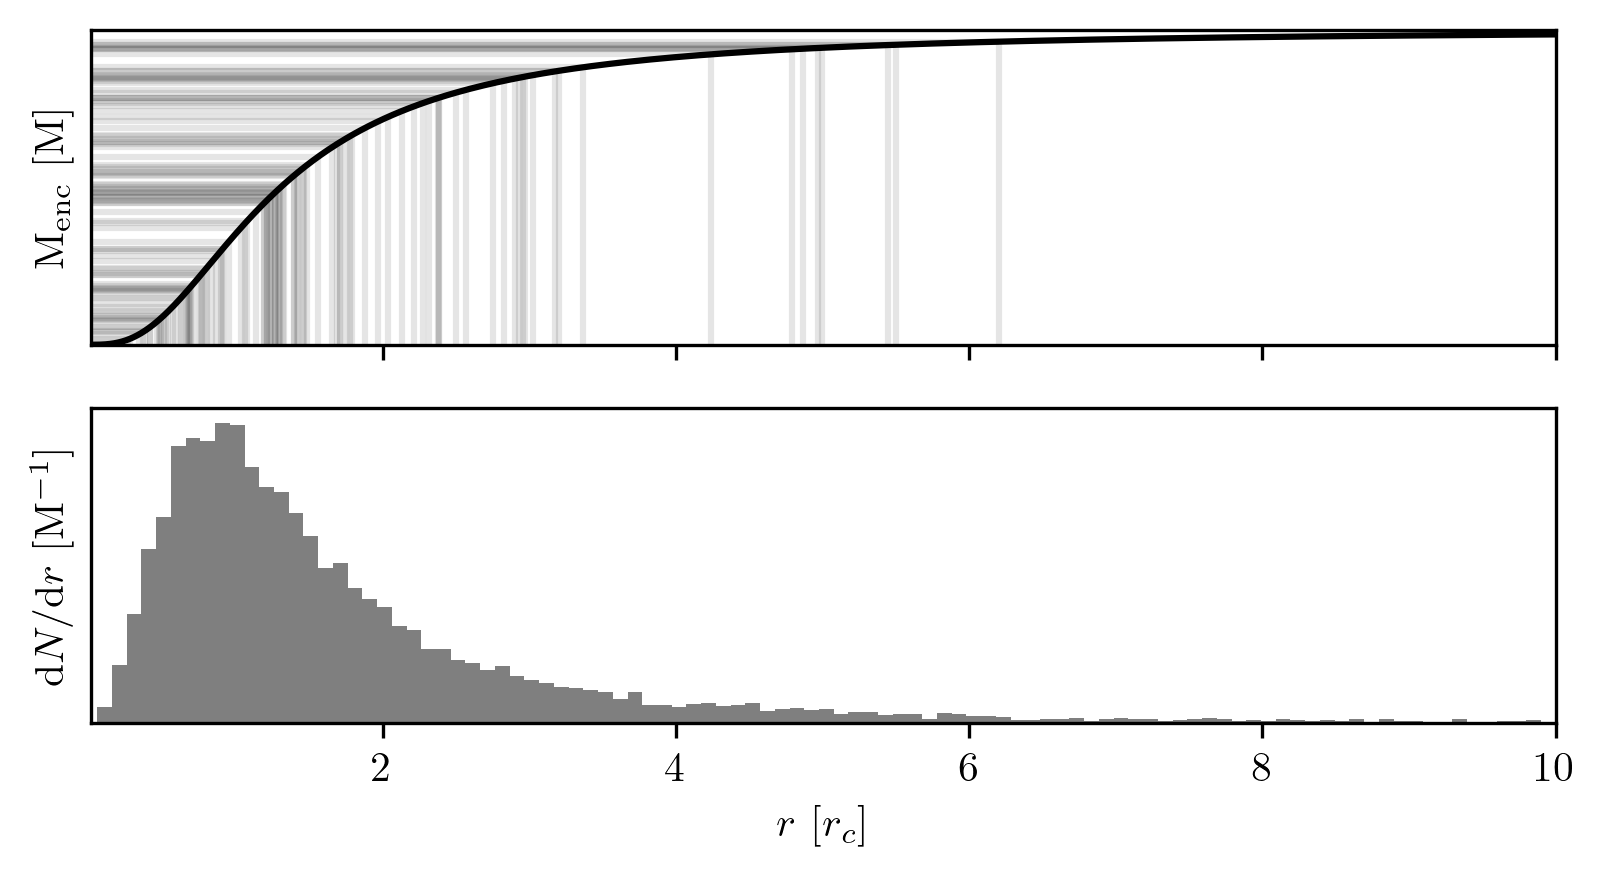
\includegraphics[width=\linewidth]{images/inverse_transform_sampling_distances.png}
                \caption[Inverse transform sampling of a marginal distribution function]{Inverse transform sampling of the enclosed mass distribution of a Plummer sphere. One thousand uniform random numbers between [0,1] were generated and intersected with the normalized enclosed mass profile. The top panel shows the sampling of positions; only 100 samples are shown to avoid overcrowding. The bottom panel shows the resulting distribution of radial distances.}
                \label{fig:inverse_transform_sampling_distances}
            \end{figure}
            The joint distribution function can be written as the product of a conditional and a marginal distribution: $f(r,v) = f(v|r) f(r)$. The number of particles at a given speed can be obtained by integrating over the angular velocity components and differentiating with respect to speed:
            \begin{equation}
                \frac{dN}{dv} = \frac{d}{dv} \int f(\textbf{v}|r)\, v^2 \sin\theta\, d\theta\, d\phi\, dv = 4\pi v^2 f(v|r).
            \end{equation}
            To construct the CDF of this conditional distribution, we must determine the appropriate limits. The allowed speed for a particle at radius $r$ ranges from zero to the escape speed, $v_{\mathrm{esc}} = \sqrt{2\Phi(r)}$. The resulting CDF is:
            \begin{equation}
                \mathcal{F}(v) = C \int_0^{v < v_\mathrm{esc}} 4\pi v^2 f(v|r) dv,
            \end{equation}
            where $C$ is a normalization constant. Although I do not present an analytical expression for $C$, it is straightforward to normalize numerically. In practice, I omit multiplicative constants and normalize a-posteriori using:
            \begin{equation}
                C = \frac{1}{\mathcal{F}(v_\mathrm{esc})}.
            \end{equation}
            Sampling the speeds is shown in Fig.~\ref{fig:inverse_transform_sampling_velocities}. Since this is a conditional distribution, each particle has its own CDF based on its position—unlike Fig.~\ref{fig:inverse_transform_sampling_distances}, where all particles are sampled from the same marginal distribution. Note that for particles located farther from the center, fewer speeds are available before they become unbound.
            \begin{figure}
                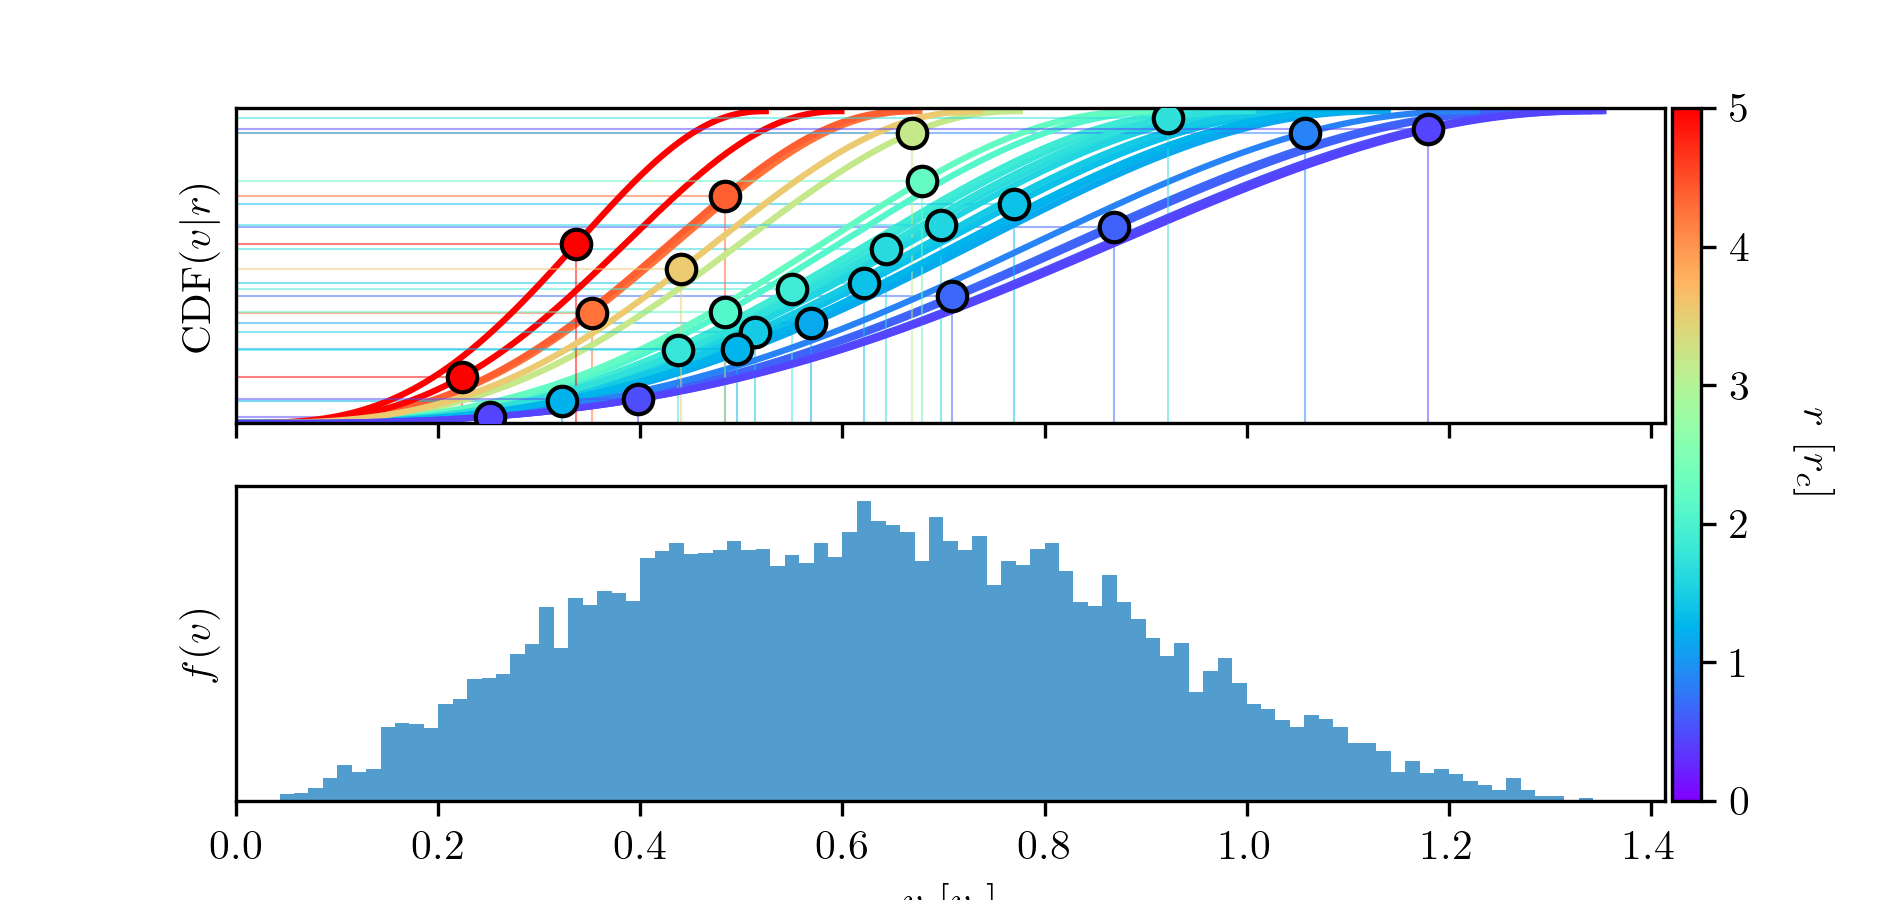
\includegraphics[width=\linewidth]{images/inverse_transform_sampling_velocities.png}
                \caption[Inverse transform sampling of a conditional distribution function]{Inverse transform sampling of the speed distribution conditioned on position for particles in a Plummer sphere ($N = 1000$). The top panel shows 25 samples (to avoid clutter), each colored by its sampled distance. For each particle, a uniform random number is mapped onto its corresponding CDF to obtain the speed. The bottom panel shows the distribution of sampled speeds. The theoretical maximum value, corresponding to the escape speed at the center, is $\sqrt{2GM/r_c}$.}
                \label{fig:inverse_transform_sampling_velocities}
            \end{figure}
            This process could be inverted: one could marginalize over position to obtain a global speed distribution, then condition on speed to sample positions. While valid, this approach is less intuitive. Most models are motivated by their density profiles, which are observable and conceptually accessible, making them a natural starting point for inverse transform sampling.
            To convert radial distances into 3D positions and speeds into velocity vectors, we must sample directions uniformly over the surface of a sphere. A common pitfall is to sample latitude and longitude uniformly, which leads to an over-density near the poles. Instead, we aim for a uniform distribution over the sphere's surface, where the differential area element is given by:
            \begin{equation}
                f(\theta,\phi)=\frac{1}{4\pi}\sin(\theta)
            \end{equation} 
            with $\theta$ the co-latitude and $\phi$ the longitude. Since $f$ does not depend on $\phi$, it can be sampled uniformly over its domain $[0, 2\pi)$. However, for $\theta$, inverse transform sampling must be used. Drawing a uniform random variable $y_i \in [0,1]$, the corresponding co-latitude is:
            \begin{equation}
                \theta_i = \cos^{-1}\left(1-2y_i\right).
            \end{equation}
            By sampling radial distances, speeds, and directions uniformly over the unit sphere, we obtain full position and velocity vectors for each particle. With these, the initial conditions for a Plummer sphere are fully specified. The user needs only to provide the total mass, characteristic radius, and the desired number of star particles.

            With the equations of motion defined, a model for the Galactic gravitational field established, a force model for the globular cluster in place, and initial conditions assigned to each star particle, we are now ready to simulate the tidal disruption of a globular cluster in the Galaxy.

\section{The Implicit Physics}
    The previous section provided everything needed to simulate the dissolution of globular clusters. However, given the equations of motion, the model for the gravitational field, and the initial conditions for both the globular clusters and their constituent stars, why should we expect stars to escape? While the formalisms in the previous section supply the necessary machinery for running simulations, they do not explain \textit{why} disruption occurs.

    In this section, I aim to describe the underlying mechanisms that cause stars to escape from globular clusters and form stellar streams. Gaining intuition for this process involves simplifying the equations \textit{even further}, in order to obtain analytical insights. I refer to this as the \textit{implicit physics}—not because it was explicitly implemented in the simulations, but because it arises naturally from the equations that be.

    To provide a brief overview: in Section~\ref{sec:thePlanarCircularRestrictedThreeBodyProblem}, I present the circular restricted three-body problem, the simplest formalism for understanding the types of motion a massless body can undergo when influenced by two significantly more massive ones, following \citet{koon2000dynamical}. In Section~\ref{sec:tidalForce}, I introduce the tidal tensor, which explains how and why the Galactic field eventually strips stars from their host clusters. This section is largely inspired by the works of \citet{2004AJ....127.2753D} and \citet{bovy_inprep}. In Section~\ref{sec:phaseMixing}, I discuss phase mixing, which describes the evolution of escaped stars and how they come to form coherent stellar streams. This treatment is also primarily based on \citet[see chapter 19.4 of][]{bovy_inprep}, although I present the phenomenon in terms of orbital energy. Finally, I introduce the study of \textit{gaps}—how perturbations can affect a stream and generate observable gaps within it. This topic is not yet formalized in textbooks and remains an active area of research. I primarily synthesize the works of \citet{2012ApJ...748...20C,2013ApJ...775...90C}, \citet{2015MNRAS.450.1136E}, \citet{2016PhRvL.116l1301B}, and \citet{2016MNRAS.457.3817S}.
    \subsection{The Planar Circular Restricted Three-Body Problem}\label{sec:thePlanarCircularRestrictedThreeBodyProblem}
        
        This section introduces the fundamental concept of the Lagrange points and regions of influence. In general, if a star is very close to the center of mass of a globular cluster, then its dynamics are determined by the cluster and the galaxy's influence is minimal. On the other hand, if the star is far from the cluster then its motion is completely described by the galaxy's gravitational field and the cluster is completely negligible. The Lagrange points are transitions between these two regime and are the points out of which the stars escape from the cluster. The magic that makes this analysis possible is decoupling the motion of the smallest body from the larger two, and studying the system in a non-inertial reference frame with a constant angular rotation rate: $\omega = 2\pi/T$, where $T$ is the orbital period of the primary and secondary. 

        To begin, even though we simplify the simulation by modeling the cluster as $\mathcal{N}$ independent three-body problems, the problem remains challenging. Indeed, if we consider all three bodies to have mass, we can write down a Hamiltonian with 18 dimensions: three positions and three momenta in $\mathcal{R}^3$ for each particle. The dimensionality of the problem can be reduced by using the conservation of total linear momentum and total angular momentum, and by expressing the dynamics in terms of relative coordinates about the system's center of mass. This reduces the total dimensionality to 9. Nevertheless, the problem remains analytically intractable due to its high dimensionality. To gain analytical insight, we simplify the system further.
        
        Instead of writing the full Lagrangian for the three-body motion, we focus on the third particle subject to the gravitational influence of the two massive bodies, in an inertial reference frame centered at the system's center of mass. The Lagrangian then contains the kinetic energy of the third particle and two gravitational potential energy terms from the primary and secondary. However, since the positions and momenta of the primaries are not treated as dynamical variables in our system, they appear as explicit functions of time, making the Lagrangian non-autonomous. This implies that the corresponding Hamiltonian is time-dependent and the total energy of the third particle is not conserved, as the primaries can exchange energy with it.

        We introduce a further simplifying assumption: the two primaries move on circular orbits. Under this assumption, we transform to a reference frame rotating with the primaries, placing them along the $x-$axis. In this rotating frame, the Lagrangian becomes autonomous; it no longer depends explicitly on time and requires no external information to determine the particle's subsequent motion.

        Two effects make this possible. First, by moving to the rotating frame, we introduce non-inertial forces: the Coriolis force and the centrifugal force. The centrifugal force is conservative, associated with a scalar potential. The Coriolis force depends on the particle's velocity as $2\omega\times v$, but because it is always perpendicular to the velocity, it does no work and thus does not change the particle's kinetic energy. After performing the coordinate transformation, the canonical momenta—now position-dependent—can be derived. The resulting Hamiltonian is:
        \begin{equation}
            \mathcal{H} = \frac{1}{2}\left(\left(p_x + \omega y\right)^2 + \left(p_y - \omega x\right)^2 \right) + \Phi_\mathrm{eff}(x,y),
        \end{equation}
        where
        \begin{equation}
            \Phi_\mathrm{eff}(x,y) = -\frac{1}{2} \omega^2 (x^2 + y^2) - \frac{G m_1}{|r_1|} - \frac{G m_2}{|r_2|}.
        \end{equation}
        The potential can be normalized by noting that the orbital angular velocity from the two-body problem satisfies \(\omega^2 = \frac{G M}{a^3}\), where \(a\) is the separation between the primaries and \(M = m_1 + m_2\) is the total mass of the system. With this normalization, the system depends on a single dimensionless parameter \(\mu\), the relative mass ratio defined as \(\mu = \frac{m_2}{m_1 + m_2}\).

        At this point, the system can be studied qualitatively. Unfortunately, no general closed-form solution exists for the circular restricted three-body problem that describes the subsequent motion as a function of time. However, by studying the effective potential \(\Phi_\mathrm{eff}\), we gain valuable insights.

        Our Hamiltonian depends on the four variables \((x, y, p_x, p_y)\) and has one integral of motion.\footnote{The term ``integral of motion'' is often used interchangeably with ``constant of motion,'' but strictly speaking, the latter is preferable, as it refers to a quantity that remains constant throughout the orbital evolution—not to an integral in the mathematical sense of the word (i.e., the area under a curve).} A well-known quantity in this context is the Jacobi integral (or Jacobi constant), often written as \(C_j = -2\mathcal{H}\). Defining this constant is somewhat arbitrary, since the non-inertial mechanical energy \(\mathcal{H}\) is itself conserved, and any scalar multiple of it is also conserved. The utility of the Jacobi constant is mostly conventional: it is often defined to be positive and multiplied by 2, which simplifies the expression for forbidden regions and zero-velocity curves. By using $p_x = \dot{x}-\omega y$ and $p_y = \dot{y} + \omega x$, one can write:
        \[
        \dot{x}^2 + \dot{y}^2 = - \left(2 \Phi_\mathrm{eff}(x,y) + C_j\right),
        \]
        instead of the equivalent:
        \[
        \dot{x}^2 + \dot{y}^2 = -2 \Phi_\mathrm{eff}(x,y) + 2 \mathcal{H}.
        \]
        Since we have four variables and one constraint, the motion is restricted to a three-dimensional hypersurface (or manifold) embedded in the four-dimensional phase space.

        At this stage, we find the points where \(\nabla \Phi_\mathrm{eff} = 0\), which correspond to the Lagrange points—locations where all effective forces balance. Of particular importance are the first two Lagrange points \(L_1\) and \(L_2\), which lie along the line connecting the primary and secondary. The effective potential at \(L_1\) is lower than at \(L_2\).

        Given a certain energy level, setting the kinetic energy to zero defines boundaries between regions where the particle can and cannot move. Regions where the kinetic energy would have to be negative (which is physically impossible) are forbidden, since that would require imaginary velocities.

        The points \(L_1\) and \(L_2\) are especially important for our study of a globular cluster with stars initially bound to it. Stars can escape through these Lagrange points: lower-energy particles tend to escape through \(L_1\), while higher-energy particles can also escape through \(L_2\). Figure~\ref{fig:CR3BP_forbidden_region} illustrates these forbidden and allowed regions clearly.
        \begin{figure}
            \centering
            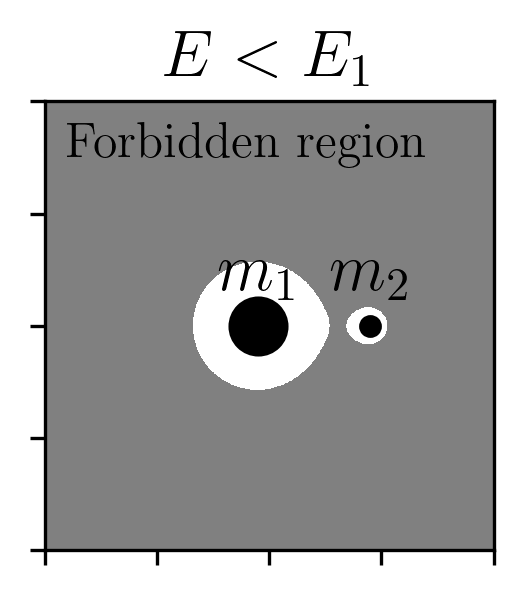
\includegraphics[width=.32\linewidth]{images/CR3BP_forbidden_region_0.png}
            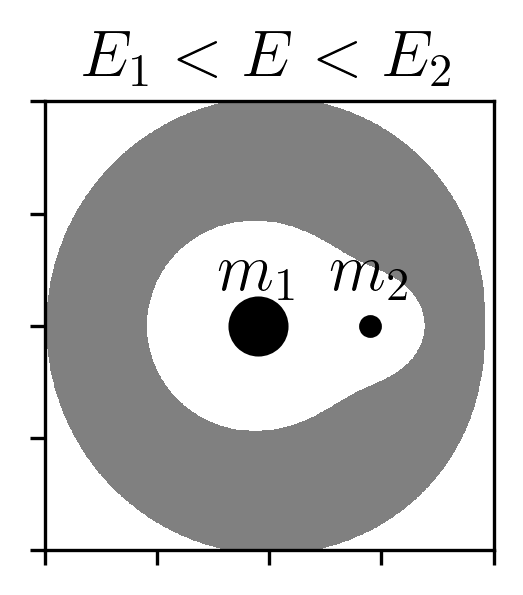
\includegraphics[width=.32\linewidth]{images/CR3BP_forbidden_region_1.png}
            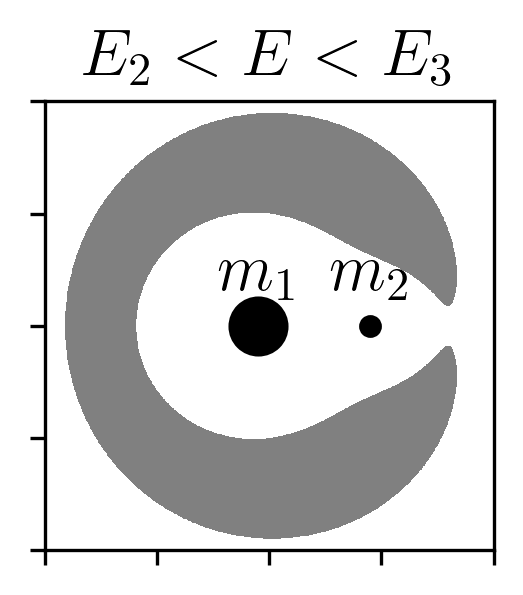
\includegraphics[width=.32\linewidth]{images/CR3BP_forbidden_region_2.png}
            
            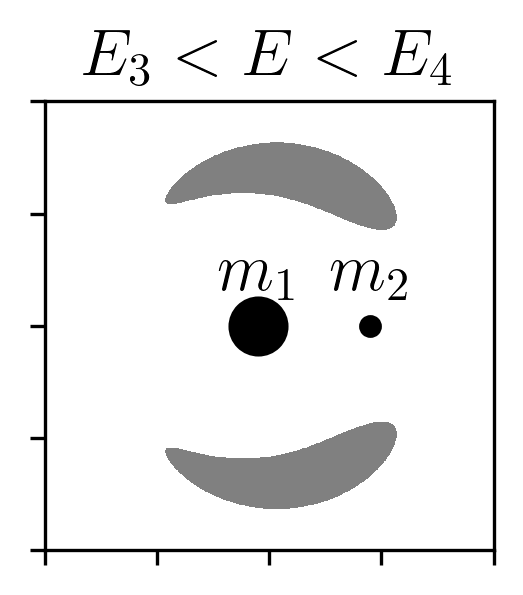
\includegraphics[width=.32\linewidth]{images/CR3BP_forbidden_region_3.png}
            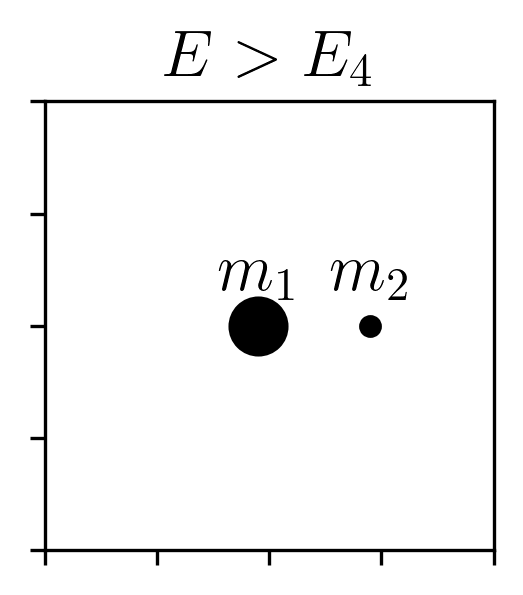
\includegraphics[width=.32\linewidth]{images/CR3BP_forbidden_region_4.png}
            \caption[Forbidden regions in the restricted three body problem]{A reproduction of Fig.~2.4.2 from \citet{koon2000dynamical}. Each plot is shown in the non-inertial reference frame rotating with the orbital frequency of the primary and secondary about their common center of mass. In this example, the mass ratio is \(m_1 = 10 m_2\). The gray regions represent areas inaccessible to the test particle for a given energy. In the first case, where \(E < E_1\), the particle remains confined to orbit either around the primary or the secondary, depending on its initial position. As the particle's energy increases, more of the \(xy\)-plane becomes accessible. The narrow passage between \(m_1\) and \(m_2\) corresponds to the \(L_1\) Lagrange point, while the choke point allowing escape to the exterior when \(E > E_2\) is the \(L_2\) point.}
            \label{fig:CR3BP_forbidden_region}
        \end{figure}
        The distance from the secondary to the first and second Lagrange points is approximately equal, defining a region around the secondary known as the Hill sphere. Within this zone, the gravitational influence of the secondary dominates over that of the primary. The Hill radius is commonly approximated as \( r_h \approx r\sqrt[3]{m_2/m_1} \), where \( r \) is the separation between the primaries. Interestingly, the expression for the Hill radius arises from a fifth-order polynomial expansion of the effective potential—a detail that might seem minor, but is actually quite delightful. In most areas of physics, approximations typically emerge from Taylor expansions, basis function decomposition's, or limits where the governing equations simplify.

        At conferences, we have been asked whether we have ever observed \textit{recapture}—that is, a star becoming bound to globular cluster. Capture is a fascinating phenomenon, particularly in the case of dark matter sub-halos that could in theory capture field stars that were not formed within them \citep{2024MNRAS.533.3263P}. If the system were as simple as the circular restricted three-body problem, recapture could occur for star particles with energies in the range \( E_1 < E < E_2 \) or \( E_2 < E < E_3 \). In such cases, depending on initial conditions, a particle might orbit the secondary, escape, and later return. However, in our simulations, the galaxy and globular clusters are not treated as point masses, and the clusters follow eccentric, inclined, and non-closed orbits. This means the topology of the forbidden region evolves over time. For a particle with a given energy \( E \), it may be unbound at one moment but later find itself within the Hill sphere again, as the potential landscape changes dynamically. Indeed, we have observed such behavior in our simulations.

        The Lagrange points, forbidden regions, and Jacobi energy are powerful concepts which, while they do not rigorously apply in our more complex setup, still offer valuable qualitative insights. In our regime, it is more fruitful to think in terms of tidal forces as the underlying mechanism that gradually transfers energy and angular momentum, nudging stars across Lagrange boundaries and ultimately enabling escape. It is to this process—tidal stripping—that we now turn.

        % \textbf{NOTE from Ferrone. I wonder if the $L_4$ and $L_5$ exist in the galactic context... are there Tojan stars? or does the complexity of the galactic potential paired with non circular orbits render such a phenomena unnatural?}

    \subsection{Tidal Forces}\label{sec:tidalForce}
        For star-particles within a globular cluster that is itself orbiting within a galaxy, there are no exact integrals of motion. The system lacks symmetries in its Lagrangian, and the potential varies with time, so even the orbital energy is not conserved. In such a time-dependent and asymmetric context, it is more insightful to frame the problem in terms of forces rather than conserved quantities. In particular, tidal forces arise when the gravitational field of the galaxy (the primary) is treated as an external perturbation to the field of the globular cluster (the secondary). In this section, I aim to build an intuitive and formal understanding of tidal forces, framing them as tensor quantities. We begin with the simplest case—the familiar Sun-Earth system—before extending the discussion to the Galactic context. I also provide a broader overview of how tidal forces vary depending on the cluster's orbit within the galaxy.

        To start, tidal forces arise due to spatial variations in the gravitational field with respect to a reference point, which is almost always the secondary body. There are two equivalent options to quantify this. The first is to consider a Taylor expansion of the gravitational potential of the primary, \(\Phi_g\), evaluated at the star's position \(\vec{x}_s\), relative to the secondary's position \(\vec{x}_c\):
        \begin{equation}
            \Phi_g\left(\vec{x}_s\right) \approx \Phi_g\left(\vec{x}_c\right) + \left[\nabla \Phi_g (\vec{x}_c)\cdot \Delta \vec{x}\right] + \left[\Delta \vec{x} \cdot \mathcal{D}^2\left(\Phi_g\right) \cdot \Delta\vec{x}\right],
        \end{equation}
        where \(\Delta \vec{x} = \vec{x}_s - \vec{x}_c\), and \(\mathcal{D}^2 \Phi_g\) is the Hessian matrix of second derivatives of the potential: \(\partial^2 \Phi/\partial x_i \partial x_j\). 

        The second expression can be derived by linearizing the gravitational force in a non-inertial frame co-moving with the secondary. Let us write Newton's second law for the star-particle and the secondary in an inertial frame:
        \begin{eqnarray}
            \vec{F}_s &= \nabla \Phi_c\left(\Delta \vec{x}\right) + \nabla \Phi_g\left(\vec{x}_s\right),\\
            \vec{F}_c &= \nabla \Phi_g\left(\vec{x}_c\right),
        \end{eqnarray}
        where $\vec{F}_s$ is the force on the secondary and $\vec{F}_c$ is the force on the secondary. Then the relative acceleration of the star in the non-inertial frame is:
        \begin{eqnarray}
            \vec{f}_s &= \vec{F}_s - \vec{F}_c + \vec{F}_\mathrm{fictitious} \\
                    &= \nabla \Phi_c\left(\Delta \vec{x}\right) + \nabla \Phi_g\left(\vec{x}_s\right) - \nabla \Phi_g\left(\vec{x}_c\right) + \vec{F}_\mathrm{fictitious} \\
                    &\approx \nabla \Phi_c\left(\Delta \vec{x}\right) + \mathrm{Jac}\left(\nabla \Phi_g(\vec{x}_c)\right) \cdot \Delta \vec{x} + \vec{F}_\mathrm{fictitious},
        \end{eqnarray}
        where the last line uses a first-order Taylor expansion of the gravitational force field, valid under the assumption that \(|\Delta \vec{x}| << |\vec{x}_c|\). 

        The Jacobian of the gravitational field is equal to the Hessian of the potential, owing to the symmetry of second derivatives and the fact that \(\vec{g} = -\nabla \Phi_g\). This matrix, known as the \textit{tidal tensor} \(\mathcal{T}\), describes the linearized spatial variation of the gravitational field:
        \begin{equation}
            \mathcal{T} = -\mathcal{D}^2\Phi_g = \mathrm{Jac}(\nabla \Phi_g) = \left(\begin{matrix}
                \partial_x g_x & \partial_y g_x & \partial_z g_x \\
                \partial_x g_y & \partial_y g_y & \partial_z g_y \\
                \partial_x g_z & \partial_y g_z & \partial_z g_z 
            \end{matrix}\right).
        \end{equation}
        While the Hessian and Jacobian are formally equivalent, the Jacobian viewpoint offers a more geometric interpretation: it acts as a linear transformation on nearby displacements, mapping them to differences in acceleration. Diagonalizing the tidal tensor reveals the principal axes of tidal deformation. A positive eigenvalue corresponds to stretching along the associated eigenvector; a negative eigenvalue indicates compression. The magnitude gives the rate of stretching or compression.

        Finally, we note that although many relevant potentials exhibit spherical or cylindrical symmetry, Cartesian coordinates are preferred here. In curvilinear systems, computing the Jacobian or Hessian requires accounting for Christoffel symbols, which complicates the interpretation and computation.
        \subsubsection{The Moon}
            Nothing clarifies the concept of tides like the most familiar example: the Moon. Tidal forces are invoked to explain a wide range of phenomena in the Earth-Moon system. The most relatable effect is, of course, the periodic variation in sea level on Earth. While accurately modeling these changes requires fluid dynamics—beyond the scope of this thesis—NASA provides several accessible explanations and visualizations at \href{https://science.nasa.gov/moon/tides/}{https://science.nasa.gov/moon/tides/}, including daily high and low tides, as well as spring and neap tides.

            Another key example is the tidal deformation of the Moon, which ultimately led to its tidal locking—explaining why we always see the same side of the Moon from Earth.

            A particularly insightful illustration is the angular offset between the Earth's tidal bulge and the Moon's position, caused by the Earth's rotation. This offset results in a torque that transfers angular momentum from the Earth's rotation to the Moon's orbit. As a consequence, Earth's rotation gradually slows while the Moon slowly recedes from Earth. 
            
            All of the above phenomena require using the tidal tensor for a Keplerian potential:
            \begin{equation}
                \mathcal{T}= -\frac{GM}{r^3}\left(\begin{matrix}
                    1-\frac{3x^2}{r^2} & -\frac{3xy}{r^2} & -\frac{3xz}{r^2} \\
                    -\frac{3yx}{r^2} & 1-\frac{3y^2}{r^2} & -\frac{3yz}{r^2} \\
                    -\frac{3zx}{r^2} & -\frac{3zy}{r^2} & 1-\frac{3z^2}{r^2}
                \end{matrix}\right),
            \end{equation}
            which has eigenvalues $2\frac{GM}{r^3}$, $-\frac{GM}{r^3}$, and $-\frac{GM}{r^3}$, with corresponding eigenvectors:
            \begin{equation}
                \vec{v}_0 = \dfrac{1}{r}\begin{bmatrix} x \\ y \\ z \end{bmatrix},\quad
                \vec{v}_1 = \dfrac{1}{\sqrt{x^2 + y^2}} \begin{bmatrix} -y \\ x \\ 0 \end{bmatrix},\quad
                \vec{v}_2 = \dfrac{1}{r\sqrt{x^2 + y^2}} \begin{bmatrix} -xz \\ -yz \\ x^2 + y^2 \end{bmatrix}.
            \end{equation}
            Notably, the first eigenvalue is positive and corresponds to stretching along the position vector $\vec{r}$. The other two eigenvalues are equal and negative, representing compression in the plane perpendicular to $\vec{r}$. Any orthonormal pair of vectors spanning this plane forms valid eigenvectors, so the choice is not unique. In this work, we illustrate this by choosing $\vec{v}_1$ perpendicular to both $\vec{r}$ and the $z$-axis, i.e., effectively projecting along $[0,0,1]$, and taking the cross product to define $\vec{v}_2$. This choice leads to a singularity when $\vec{r}$ is aligned with the $z$-axis; in that case, any other reference axis can be chosen to define the perpendicular plane.
            
            From this, several tidal effects become evident. For instance, the Earth's oceans stretch along the Earth-Moon axis due to the Moon's tidal forces. While the Sun also exerts tidal forces on Earth, their magnitude is weaker due to the $r^{-3}$ scaling with distance. When the Moon is either full or new, the Sun and Moon's tidal forces act constructively, leading to spring tides. At first and third quarters, they interfere destructively, causing neap tides. Additionally, Earth's tidal influence distorts the Moon from spherical symmetry into an ellipsoid. The Moon's most stable orientation is one where its longest axis aligns with the Earth-Moon line—resulting in tidal locking.

            A more quantitative treatment of these phenomena would require modeling the Moon's internal structure and Earth's ocean dynamics—well beyond the gravity-only scope of this thesis. However, we can still explore one instructive effect: how solar tidal forces \textit{perturb} the Moon's orbit away from the idealized two-body Earth-Moon configuration. Figure~\ref{fig:moon_tidal_simulation} shows a toy model comparing two scenarios. In both, I used initial conditions based on JPL NASA ephemerides \citep{2014IPNPR.196C...1F} and integrated two sets of equations of motion. Neglecting solar tides causes the predicted Moon orbit to drift ahead of the more accurate trajectory. With about three to four years, the two body predicted solution would off by half a moon phase. 

            In the first scenario, the Moon's motion is governed by the two-body Earth-Moon problem with a rotating reference frame correction:
            \begin{equation}
                \ddot{\vec{r}} = -\frac{GM_\oplus}{r^3}\vec{r} - \omega_\oplus \times \left(\omega_\oplus \times \vec{r}_\oplus\right),
            \end{equation}
            while in the second, we include the effect of solar tidal forces:
            \begin{equation}
                \ddot{\vec{r}} = -\frac{GM_\oplus}{r^3}\vec{r} - \omega_\oplus \times \left(\omega_\oplus \times \vec{r}_\oplus\right) -\frac{GM_\odot}{r_\oplus^3}
                \left(\begin{matrix}
                    1-\frac{3x^2}{r_\oplus^2} & -\frac{3xy}{r_\oplus^2} & -\frac{3xz}{r_\oplus^2} \\
                    -\frac{3yx}{r_\oplus^2} & 1-\frac{3y^2}{r_\oplus^2} & -\frac{3yz}{r_\oplus^2} \\
                    -\frac{3zx}{r_\oplus^2} & -\frac{3zy}{r_\oplus^2} & 1-\frac{3z^2}{r_\oplus^2}
                \end{matrix}  \right) \cdot \vec{r},
            \end{equation}
            where $r_\oplus$ is the Earth's position relative to the Sun, $\vec{r}$ is the Moon's position relative to Earth, $M_\odot$ is the mass of the Sun, and $M_\oplus$ is the mass of the Earth. The coordinates $x, y, z$ refer to the components of Earth's heliocentric position.

            % \begin{verbatim}
            % VIDEO: moon_tidal_simulation.mp4
            % \end{verbatim}

            \begin{figure}
                \centering
                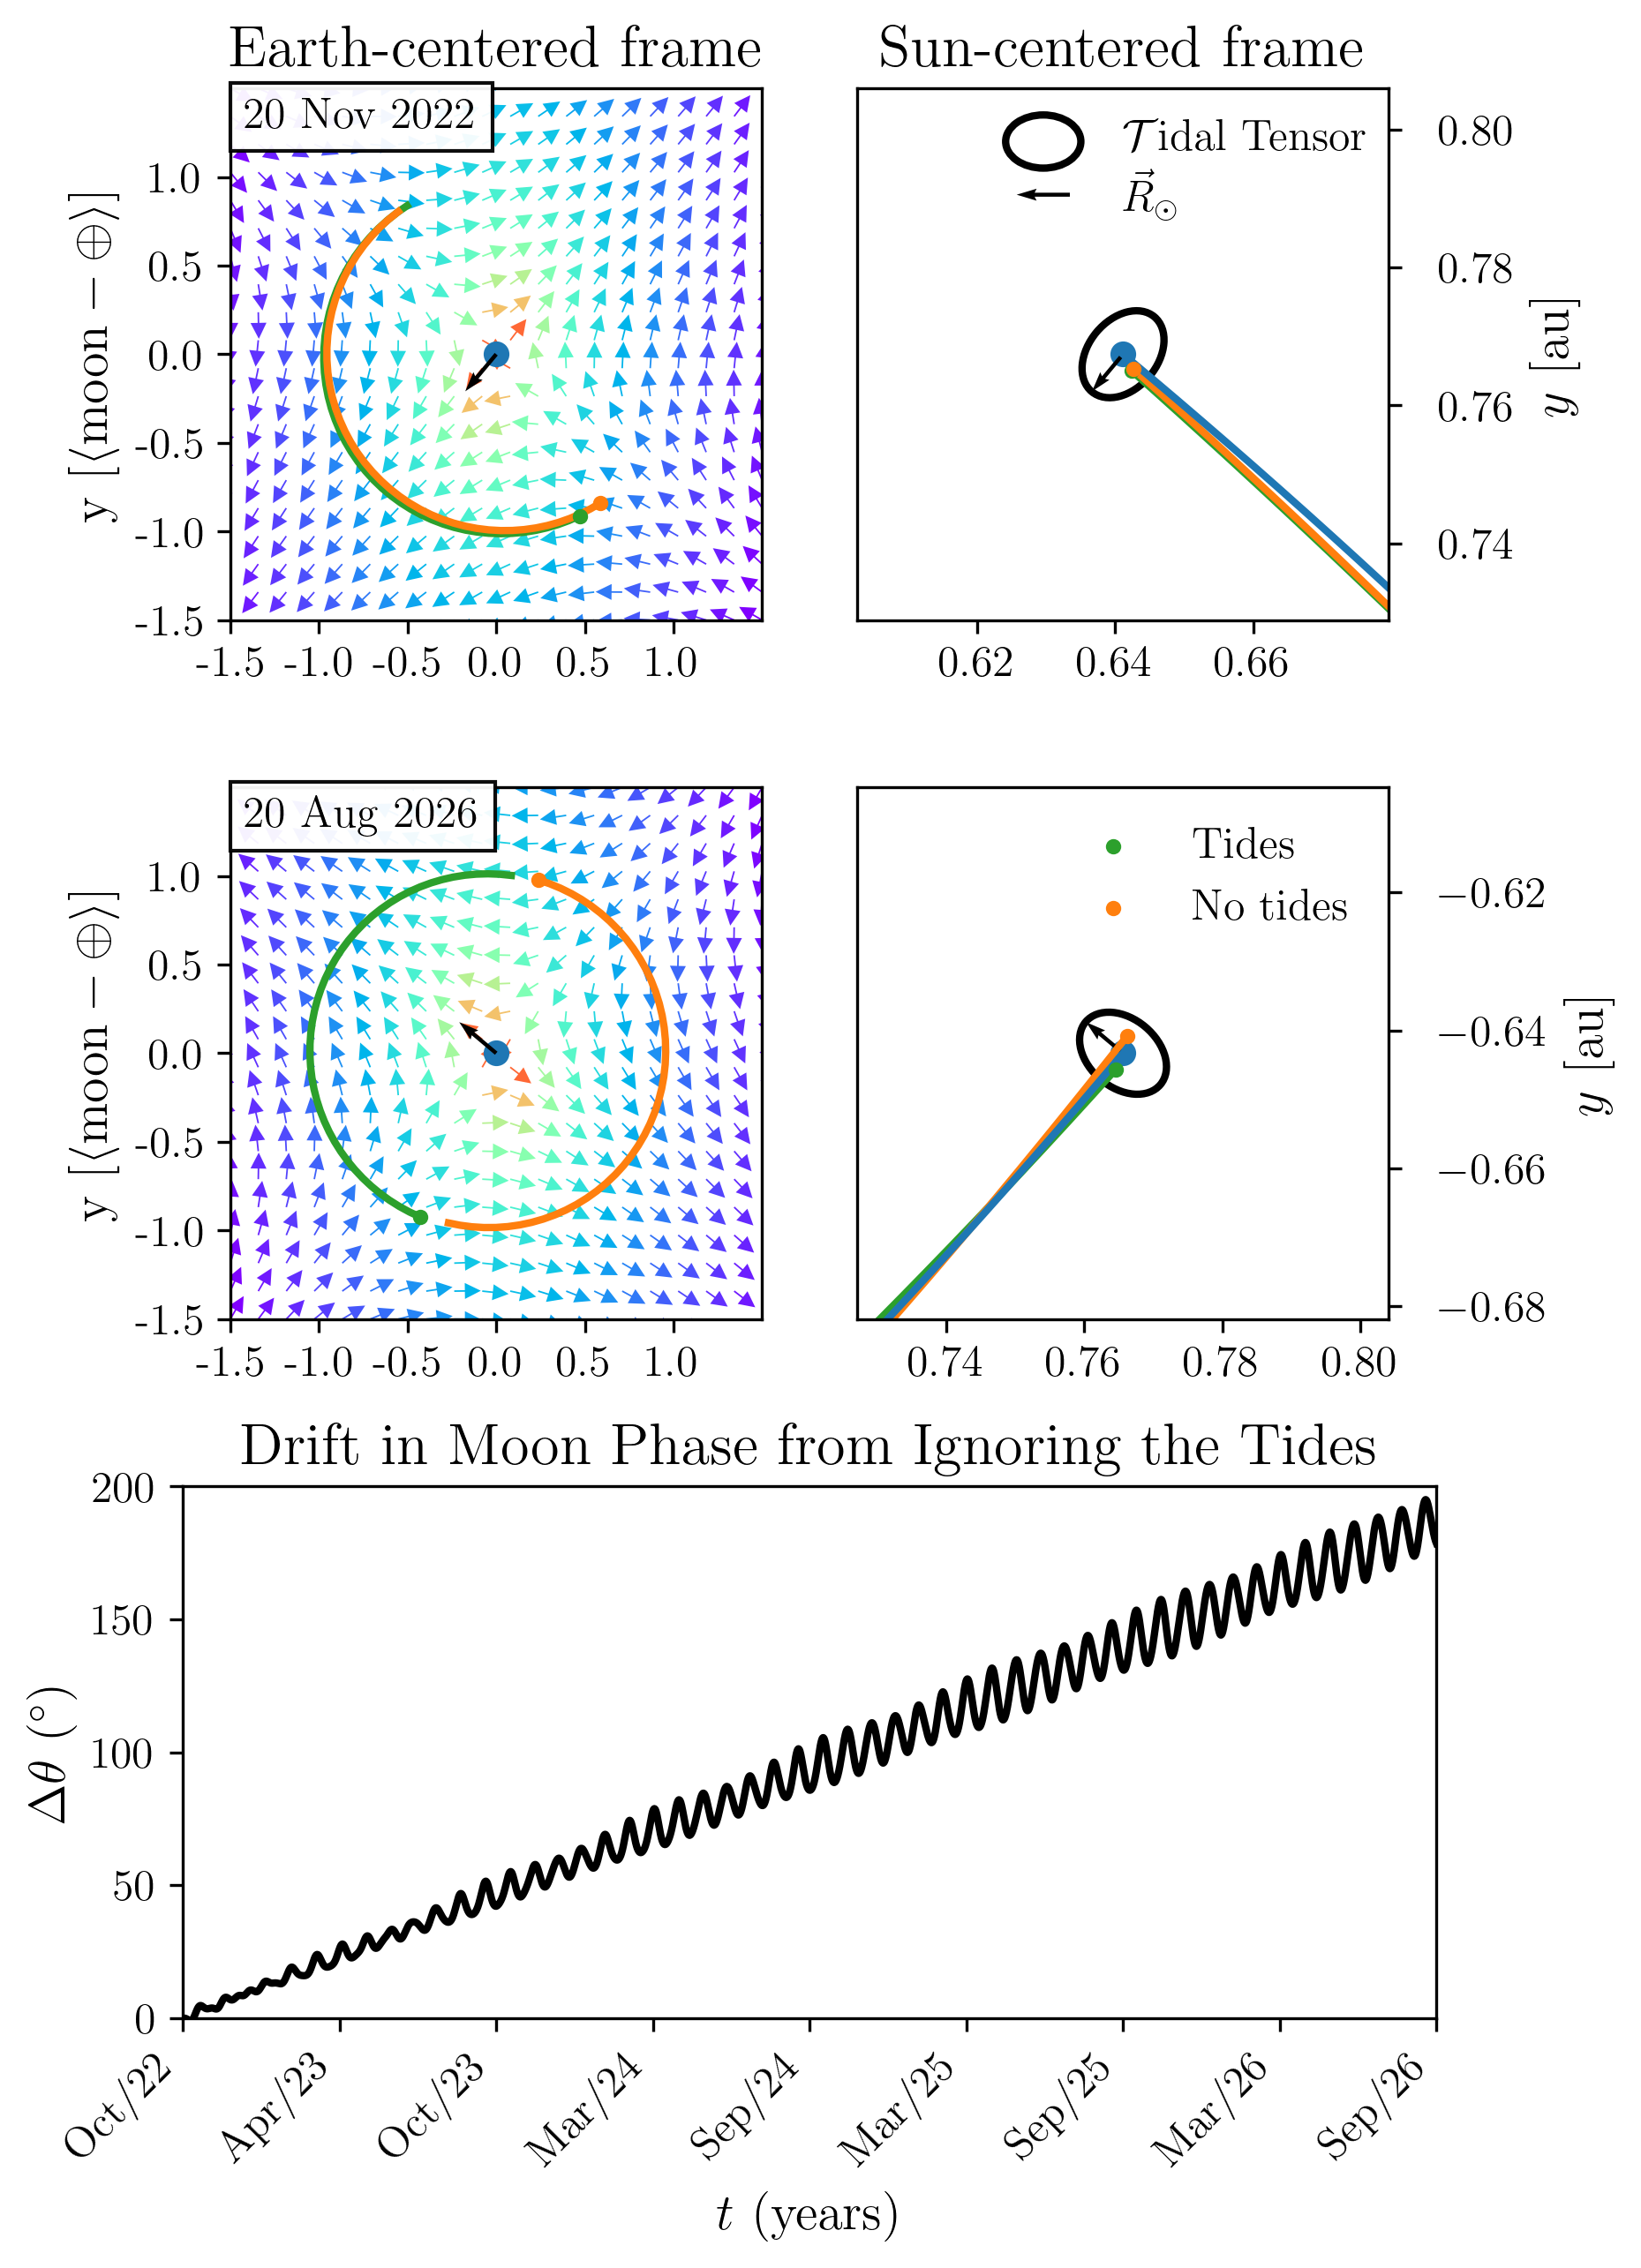
\includegraphics[width=.8\linewidth]{images/moon_tidal_simulation.png}
                \caption[Effects of Solar tides on the lunar orbit]{An illustrative experiment demonstrating the effect of the Sun's tidal field. The left panels show the tidal field, and the right panels show two snapshots of the Moon's orbital trajectory. The green curve include the Sun's tidal effects, while the orange curve corresponds neglects them. The black ellipse represents the tidal ellipsoid, whose major axis aligns with the Sun's position vector relative to the Earth. The bottom panel shows the accumulated phase difference between the two solutions. }\label{fig:moon_tidal_simulation}
            \end{figure}

        \subsubsection{Tides from the disk}
            In the Milky Way, the disk, bulge, and halo each contribute differently to the tidal forces experienced by a globular cluster. The Miyamoto-Nagai disk produces strong, rapidly varying tidal fields near the Galactic plane, leading to phenomena such as disk shocking when clusters cross the disk. The Allen-Santillan halo, on the other hand, provides a more slowly varying, generally weaker tidal field at large Galactocentric radii.

            The strength and orientation of the tidal field at a cluster's location determine both the rate at which stars are stripped and the geometry of the resulting stellar streams. For example, clusters on eccentric or inclined orbits experience time-dependent tidal forces, with strong compressive shocks during disk crossings and enhanced stretching near pericenter. The eigenvalues and eigenvectors of the tidal tensor at each point along the orbit reveal the principal axes of stretching and compression, which in turn set the directions along which stars are most likely to escape.

            By computing the tidal tensor for the Miyamoto-Nagai disk and Allen-Santillan halo potentials, as shown below, we can visualize and quantify these effects. The following figures illustrate how the tidal field evolves for representative orbits, highlighting the interplay between the cluster's trajectory and the Galactic mass distribution. This analysis underpins our understanding of stream formation and the morphological diversity of observed tidal tails.

            We can construct the tidal tensor for the Miyamoto-Nagai potential. First, it is convenient to non-dimensionalize the potential. Below, we normalize the potential by the total mass and gravitational constant, $\Phi^\prime = \Phi / (GM)$, and each distance by the characteristic length of the disk, $x^\prime = x/a$, $b^\prime = b/a$. For clarity, we omit the prime notation in what follows. The dimensionless potential then becomes:            
            \begin{eqnarray}
                \Phi   &= \frac{1}{D},\\
                D       &= \sqrt{x^2 + y^2 + \beta^2(z)},\\
                \beta(z)   &= 1 + \sqrt{z^2 + b^2}.
            \end{eqnarray}
            The dimensionless tidal tensor is then: 
            \begin{equation}
                \mathcal{T}=-\frac{1}{D^3}\left(\begin{matrix}
                    1-\frac{3x^2}{D^2} & -\frac{3xy}{D^2} & -\frac{3x\beta \beta'}{D^2} \\
                    \dots & 1-\frac{3y^2}{D^2} & -\frac{3y\beta \beta'}{D^2} \\
                    \dots & \dots & \beta'^2 + \beta \beta'' -\frac{3\left(\beta\beta'\right)^2}{D^2}
                \end{matrix}\right),
            \end{equation}             
            where $\beta^\prime = \frac{d \beta}{dz}$ and $\beta^{\prime\prime} =  \frac{d^2 \beta}{dz^2}$. We immediately notice that, due to the cylindrical symmetry, the eigenvectors are not as simple as in the spherical case. As long as 
            \[
            \beta'^2 + \beta \beta'' - \frac{3\left(\beta \beta'\right)^2}{D^2} \neq 1 - \frac{3z^2}{D^2},
            \]
            (1) the stretching axis is no longer parallel to the position vector, and (2) the compression axes do not necessarily lie in the same plane—they may instead be fixed in orientation and differ in magnitude. The exact orientation of all three eigenvectors depends on the cluster's position in the galaxy. Note that if $z = 0$, we recover the case where the stretching eigenvector is parallel to the position vector, although the compression axes remain unequal in magnitude and fixed in orientation. If instead $b = 0$, then we recover spherical symmetry, and the compression eigenvalues become equal.
            % \begin{verbatim}
            % VIDEO: tidal_deformation_ellipsoid.mp4
            % \end{verbatim}
            I have prepared Figs.~\ref{fig:miyamoto_disc_shocks_circular_inclined_orbit}-\ref{fig:miyamoto_disc_shocks_weak_shocks} to illustrate the diversity of tidal forces experienced by clusters on various orbits within a Miyamoto-Nagai disk potential. I generate initial conditions with prescribed pseudo-eccentricities and inclinations. Each initial condition is set at apocenter, specified by a radial distance and an inclination from the disk plane. The initial velocity vector is oriented perpendicular to both the z-axis and the position vector. The circular speed at the initial position is computed as $v_\mathrm{circ} = \sqrt{|\mathbf{r}| \cdot |\nabla\Phi(\mathbf{r})|}$. The pseudo-eccentricity is applied via $v_0 =  v_\mathrm{circ} \sqrt{\frac{1 - e}{1 + e}}$.

            Fig.~\ref{fig:miyamoto_disc_shocks_circular_inclined_orbit} shows a cluster on an inclined, non-eccentric orbit. In contrast, Fig.~\ref{fig:miyamoto_disc_shocks_planar_eccentric_orbit} presents a planar but eccentric orbit. The former experiences repeated disk shocks, while the latter undergoes enhanced tidal forces primarily near pericenter passages.

            Fig.~\ref{fig:miyamoto_disc_shocks_resonant_R_z} presents an orbit in which the radial and vertical oscillation periods are nearly resonant, producing two disk shocks per pericenter passage. Fig.~\ref{fig:miyamoto_disc_shocks_big_apocenter} shows a cluster on an orbit with a large apocenter, resulting in very weak tidal forces overall. Finally, Fig.~\ref{fig:miyamoto_disc_shocks_weak_shocks} demonstrates a case with a very thick disk potential. In this case, disk shocks occur over longer timescales and are less abrupt.
            \begin{figure}
                \centering
                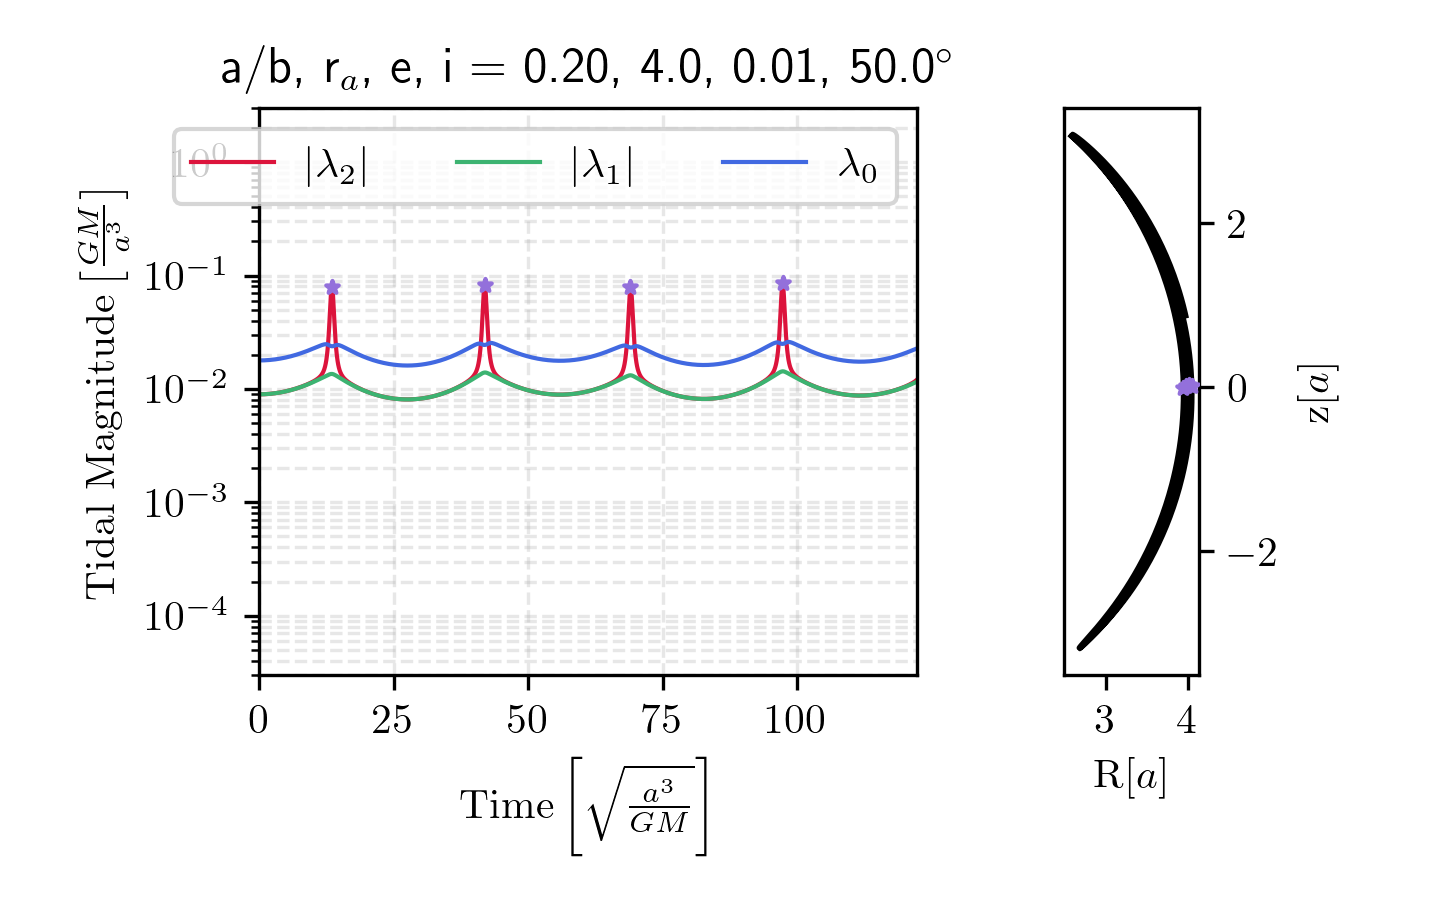
\includegraphics[width=.9\linewidth]{images/miyamoto_disc_shocks_ab_rp_e_i_0.20_4.0_0.01_50.0.png}
                \caption[Disk tidal forces on an inclined circular orbit]{Tidal forces on an inclined yet non-eccentric orbit. Disk shocks are present, yet there is no tidal stretching from pericenter passages. \textbf{Left}: The three eigenvalues of the tidal tensor matrix are plotted against time. Both the forces and time are normalized to the characteristic values of the Miyamoto-Nagai model, where $a$ is the radial scale length and $M$ is the total mass of the system. The red and green curves correspond to the two compressive axes, while the blue curve shows the magnitude of the stretching axis. The parameters listed at the top describe the orbit: the ratio of cylindrical to vertical scale lengths, the apocenter distance, the eccentricity, and the initial orbital inclination. \textbf{Right}: The orbit is shown in the meridional plane. The purple stars indicate disk crossing events and correspond to the peaks in the magnitude of the eigenvalues. }
                \label{fig:miyamoto_disc_shocks_circular_inclined_orbit}
            \end{figure}

            \begin{figure}
                \centering
                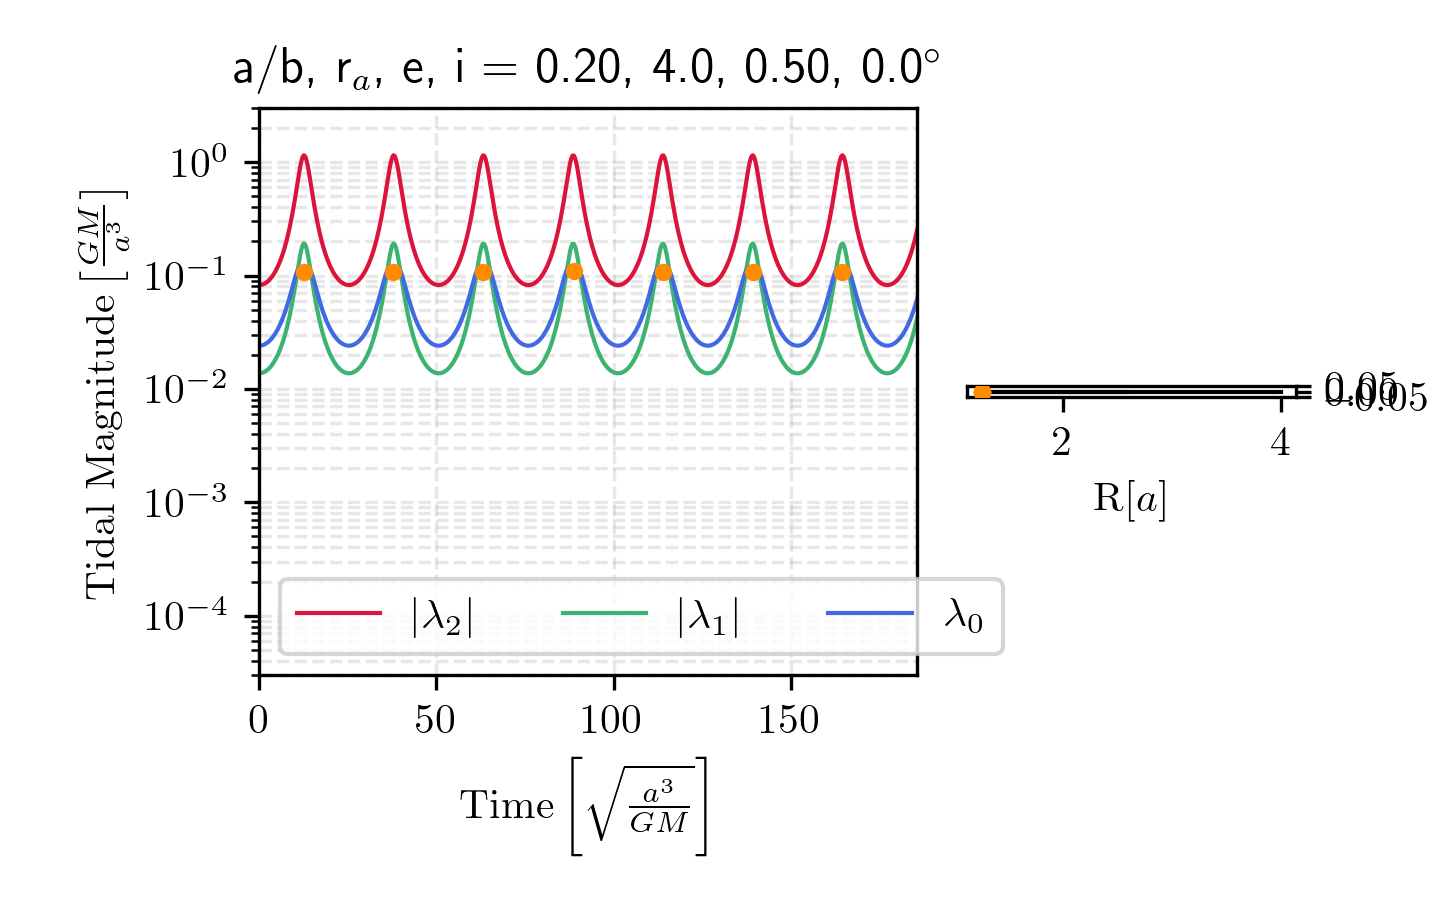
\includegraphics[width=.9\linewidth]{images/miyamoto_disc_shocks_ab_rp_e_i_0.20_4.0_0.50_0.0.png}
                \caption[Disk tidal forces on an eccentric planar orbit]{Same as Fig.~\ref{fig:miyamoto_disc_shocks_circular_inclined_orbit}. Evolution of the tidal eigenvectors for an eccentric, non-inclined orbit, resulting in a compressed meridional plane. Orange dots mark the pericenter passages. Since the cluster remains confined to the plane, no disk shocks occur.}
                \label{fig:miyamoto_disc_shocks_planar_eccentric_orbit}
            \end{figure}

            \begin{figure}
                \centering
                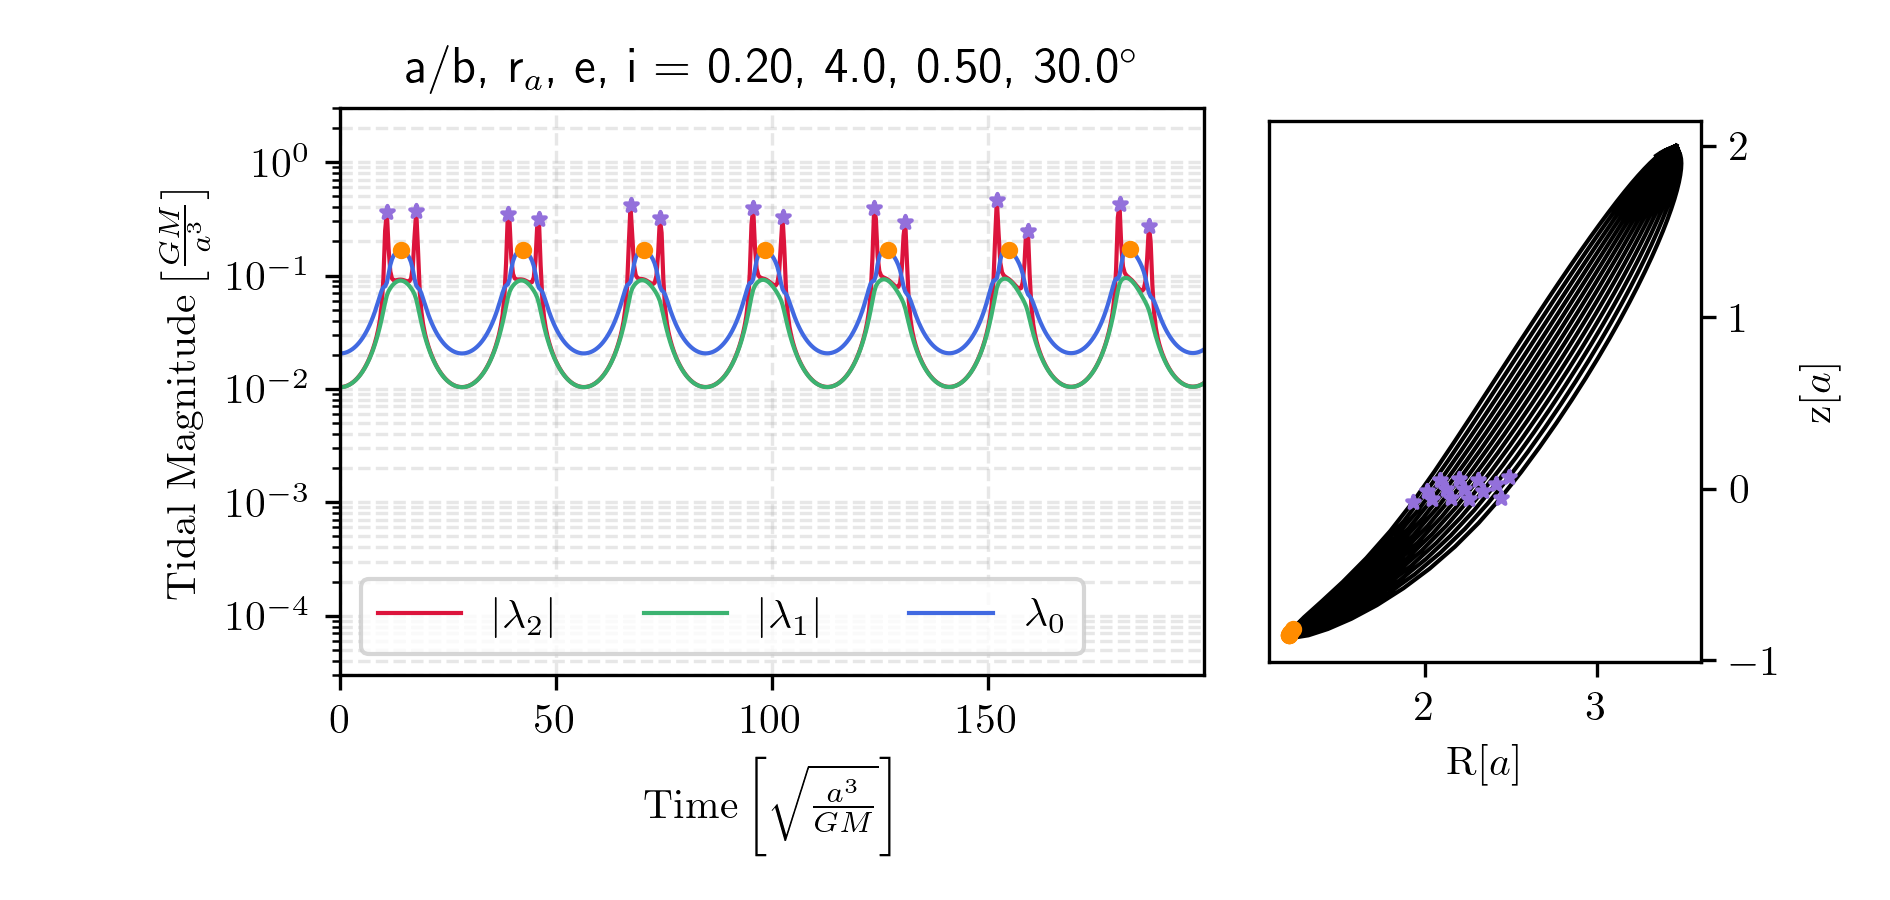
\includegraphics[width=.9\linewidth]{images/miyamoto_disc_shocks_ab_rp_e_i_0.20_4.0_0.50_30.0.png}
                \caption[Disk tidal forces on a resonant inclined and eccentric orbit]{An inclined, eccentric orbit in which the frequencies in both the $R, p_R$ and $z, p_z$ planes are nearly resonant. The axis are the same as: Fig.~\ref{fig:miyamoto_disc_shocks_resonant_R_z}. The cluster crosses the disk just before and just after each pericenter passage. This is the same orbit as the video presented in this section that is available in the online version.}
                \label{fig:miyamoto_disc_shocks_resonant_R_z}
            \end{figure}
            
            \begin{figure}
                \centering
                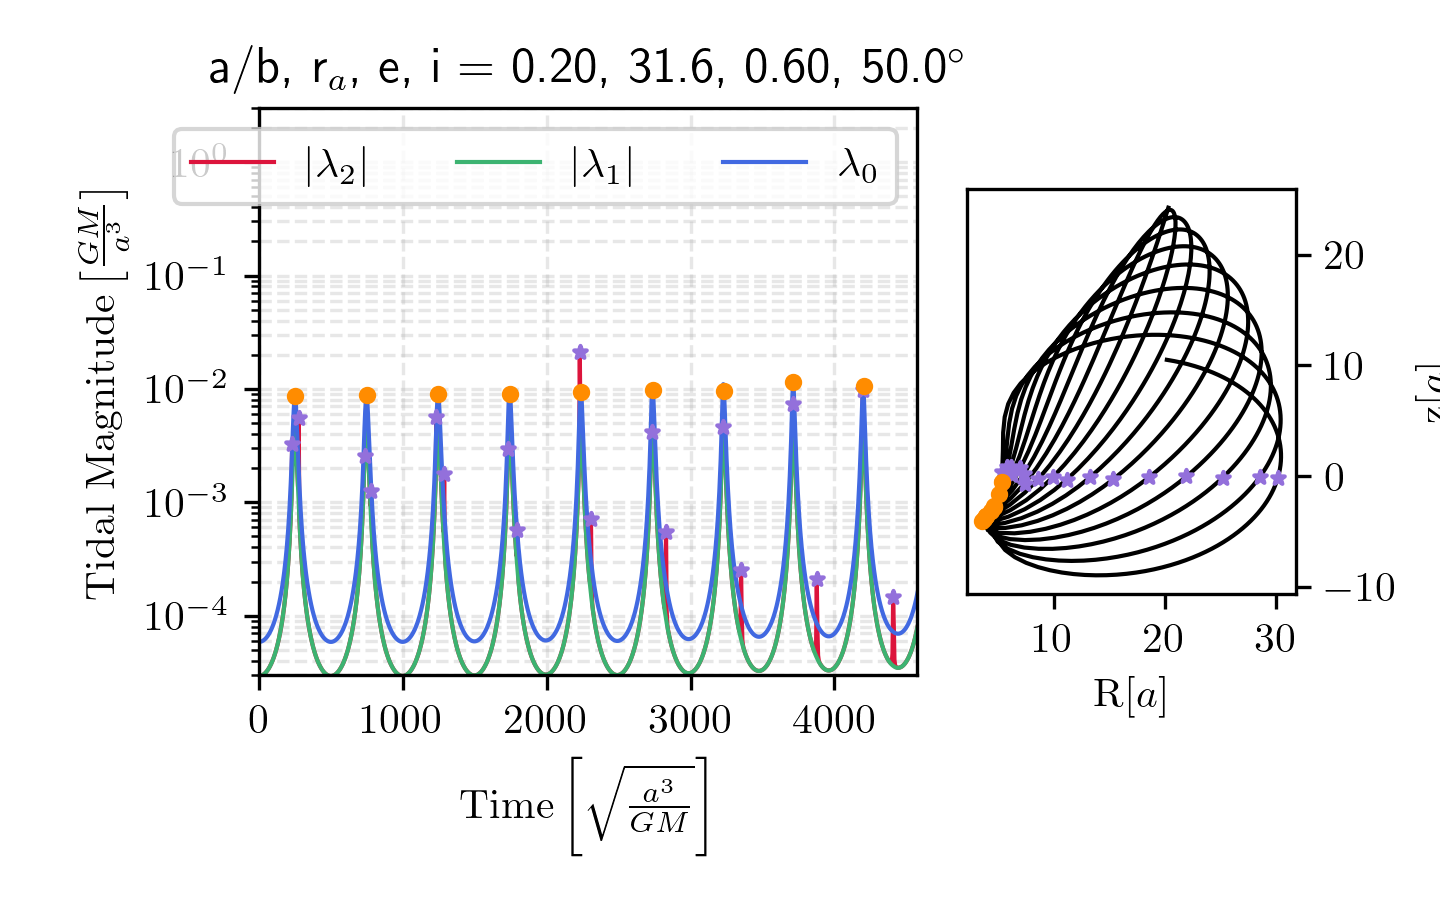
\includegraphics[width=.9\linewidth]{images/miyamoto_disc_shocks_ab_rp_e_i_0.20_31.6_0.60_50.0.png}
                \caption[Disk tidal forces on an eccentric, inclined orbit with a large apocenter]{ As the cluster evolves through phase space, disk crossings that occur farther out happen at steeper angles and in lower-density regions, reducing the strength of the resulting disk shocks. In contrast, crossings near pericenter remain strong. Because this orbit has higher energy than the previous cases, the overall magnitude of the tidal forces is lower. }
                \label{fig:miyamoto_disc_shocks_big_apocenter}
            \end{figure}
            
            \begin{figure}
                \centering
                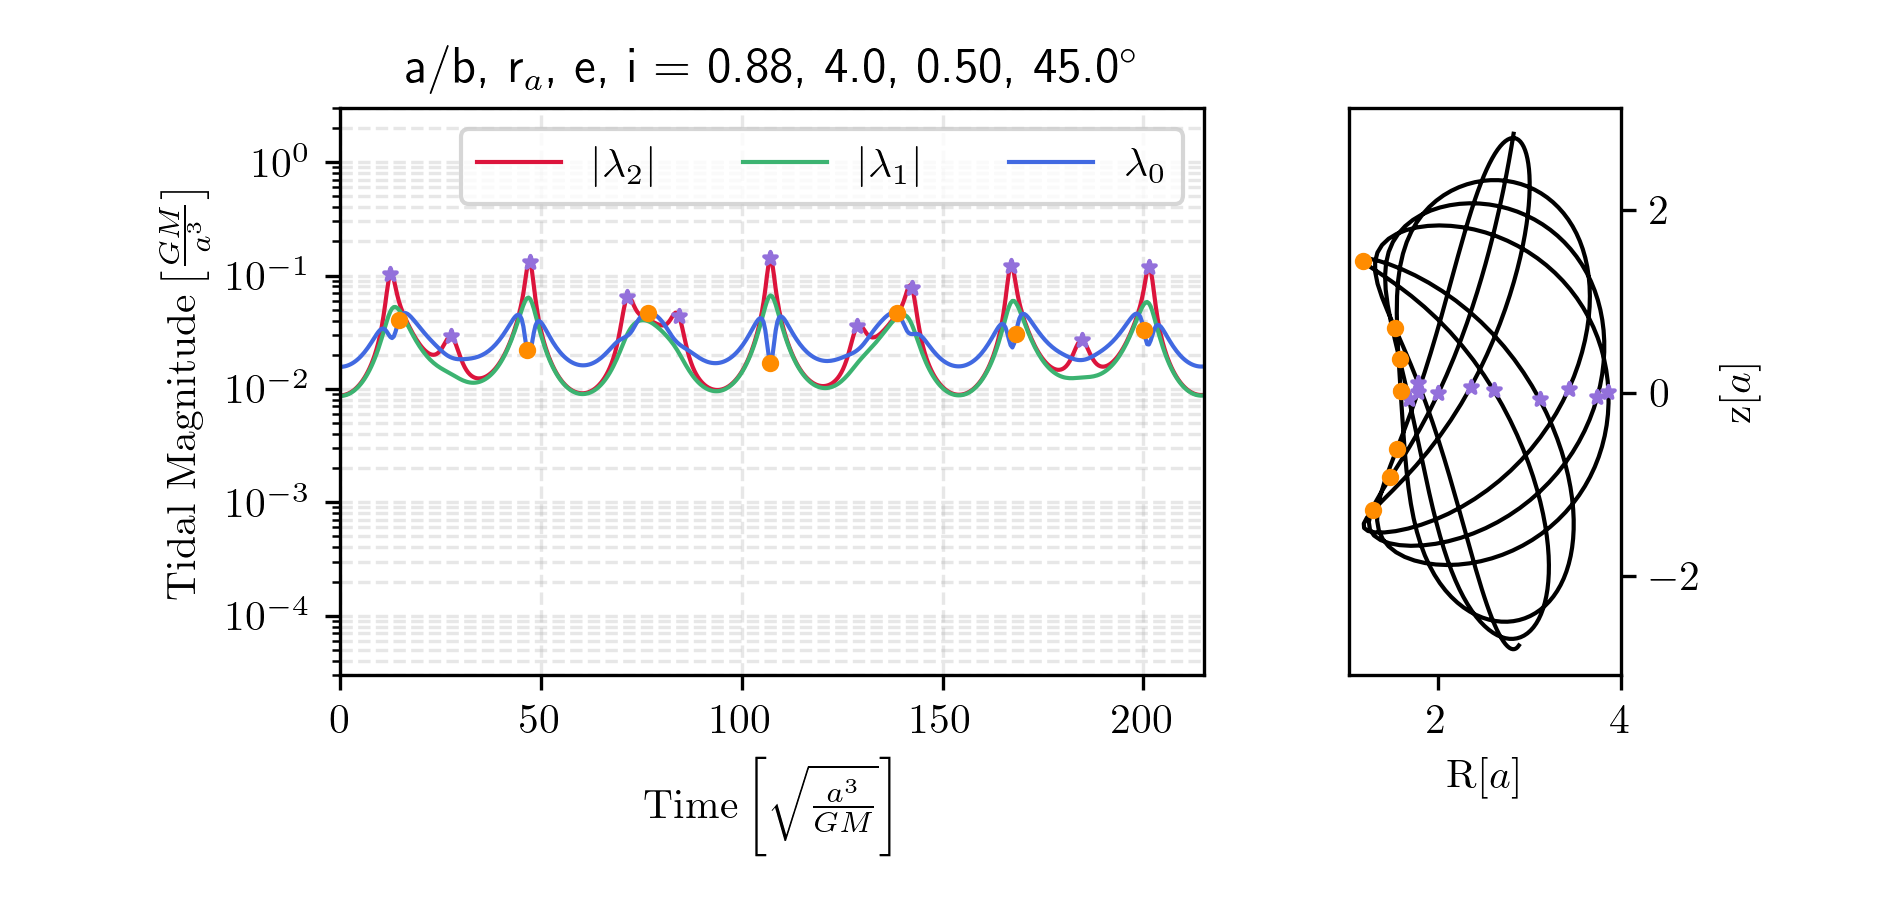
\includegraphics[width=.9\linewidth]{images/miyamoto_disc_shocks_ab_rp_e_i_0.88_4.0_0.50_45.0.png}
                \caption[Disk tidal forces on an eccentric and inclined orbit with a very thick disk]{Eccentric and inclined orbit in a weak disk. The ratio of the cylindrical scale length  to characteristic height (a/b) is close to 1. The disk crossings still produce significant tidal compression, but the resulting shocks are broader.}
                \label{fig:miyamoto_disc_shocks_weak_shocks}
            \end{figure}

        \subsubsection{Tides from the dark matter halo}
            Given spherical symmetry, we expect the tidal tensor of the halo to be similar to that of a Keplerian tidal tensor. Perhaps the magnitude of the tidal forces will not scale as simply with $\propto r^{-3}$, since the mass is not concentrated in a single point. However, we can still expect the stretching axis to be parallel with the position vector. 
            
            To explore this, first we rewrite equation~\ref{eq:martos_enclosed_mass}, the mass distribution of the Allen-Santillan halo \citep{1986RMxAA..13..137A,1991RMxAA..22..255A}, in a non-dimensional form:
            \begin{equation}
                M'_\text{enc}(s) = \frac{s^\gamma}{1+s^{\gamma-1}},
            \end{equation}
            where $\gamma$ is the exponential slope parameter, $s$ is the radial distance scaled to the characteristic radius $r_0$ and $M'$ is the enclosed mass normalized to the mass parameter: $M_\mathrm{enc}/M_0$. From Poisson's equation in spherical symmetry: the force is: $\nabla \Phi = - M_\mathrm{enc}/r^2$. The dimensionless tidal tensor can be written as: 
            \begin{equation}
                \mathcal{T'}= -\frac{M'_\text{enc}(s)}{s^3}\left(\begin{matrix}
                    1-\frac{x^2}{s^2}f(s) & -\frac{xy}{s^2}f(s) & -\frac{xz}{s^2}f(s) \\
                    -\frac{yx}{s^2}f(s) & 1-\frac{y^2}{s^2}f(s) & -\frac{yz}{s^2}f(s) \\
                    -\frac{zx}{s^2}f(s) & -\frac{zy}{s^2}f(s) & 1-\frac{z^2}{s^2}f(s)
                \end{matrix}\right)
            \end{equation}  
            where 
            \begin{equation}
                f(s) = 2-\frac{\gamma-1}{1+s^{\gamma-1}}.
                \label{eq:martos_f_s}
            \end{equation}
            While exploring this tidal tensor, I came across an interesting area of the parameter space, that I would like to show here. 

            Taking the Allen-Santillan tidal tensor in Eq.~\ref{eq:martos_f_s}, we can see that for $\gamma > 3$ and $s <  1$, then $f(s)< 0$. Physically, this would be a sphere whose density increases with distance. This is not natural, as, in general, gravity sends the more massive objects towards the center. However, it is interesting to indulge in this situation to learn some insight about the flexibility of tidal fields. The consequence of $f(s)< 0$ is that all terms in the tidal tensor are negative, which means that the force is compressive everywhere. Consequently, no stars escape from the cluster. 

            In Fig.~\ref{fig:martos_tidal_field_small_r}, I present a small experiment demonstrating the consequence of such a tidal force on a globular cluster, which is that no tidal stream forms. Briefly, I created a Plummer sphere of $10^6$~M$_\odot$ and half mass radius 20~pc and evolved it in a Allen-Santillan halo potential of mass parameter $10^{12}$~M$_\odot$ a characteristic radius of $30$~kpc. Each cluster was placed at the same initial conditions, a distance of 1/4 the scale radius from the center of the potential. The initial velocity was made perpendicular to the position vector with a speed of $(1-e)v_\textrm{c}$. This is a pseudo-eccentricity, which was added to have a non-circular orbit to demonstrate how the trajectories change in the two cases. The top panel uses a $\gamma$ of 2.02, which is the same value in the model where the halo was originally presented, and the value I employ in this thesis. Next, the bottom panel uses $\gamma$ of 4.5, which corresponds to a density profile where $\rho(r) \propto r^{1.5}$. 

            To get a feel for the strength of the tidal stretching and compression, I apply the tidal deformation to a circle and show the resulting ellipse, as shown by the black lines in the right panels of Fig.~\ref{fig:martos_tidal_field_small_r} and Fig.~\ref{fig:martos_tidal_field_big_r}. I computed the coordinates of the ellipse by adding 
            \begin{equation}
            \vec{Ell} = \vec{C} + \frac{1}{2} t_\textrm{char}^2 \mathcal{T}\cdot \left(\vec{C} - \vec{r_o}\right).
            \end{equation} 
            This way, force can be mapped to position space, and the strengths of the tidal forces can be seen visually. The characteristic time, $t_\textrm{char}$, is a free parameter that scales the deformation. I choose to set it to $\frac{1}{10} 2\pi r_\textrm{halo} / v_\textrm{c}$. 
            \begin{figure}
                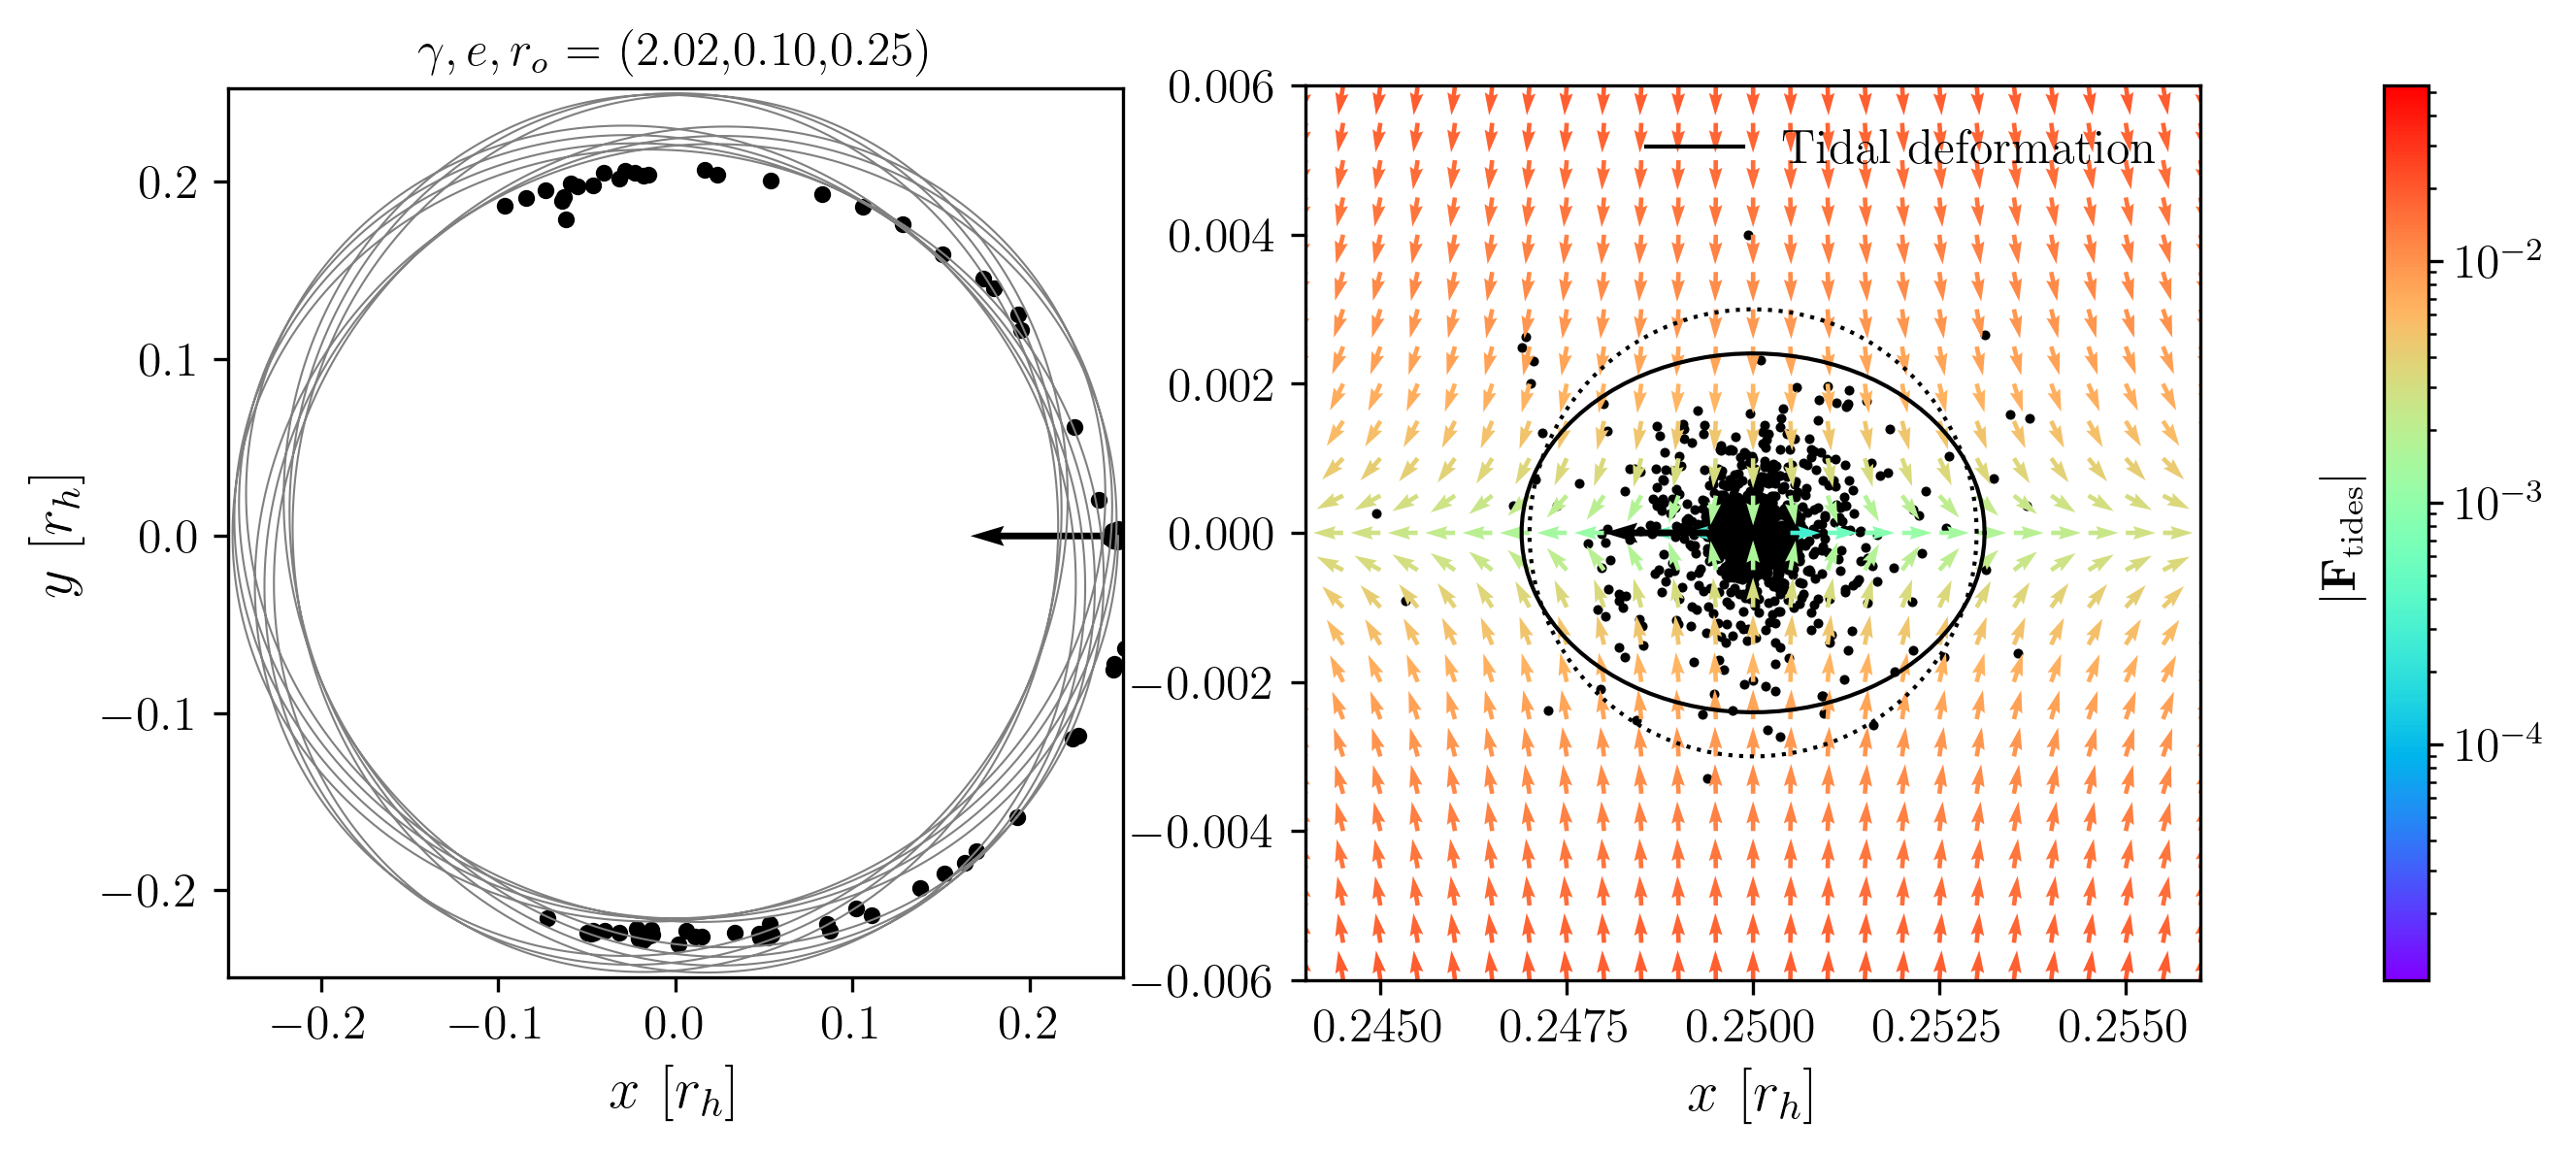
\includegraphics[width=\linewidth]{images/martos_tidal_field_202_10_25.png}
                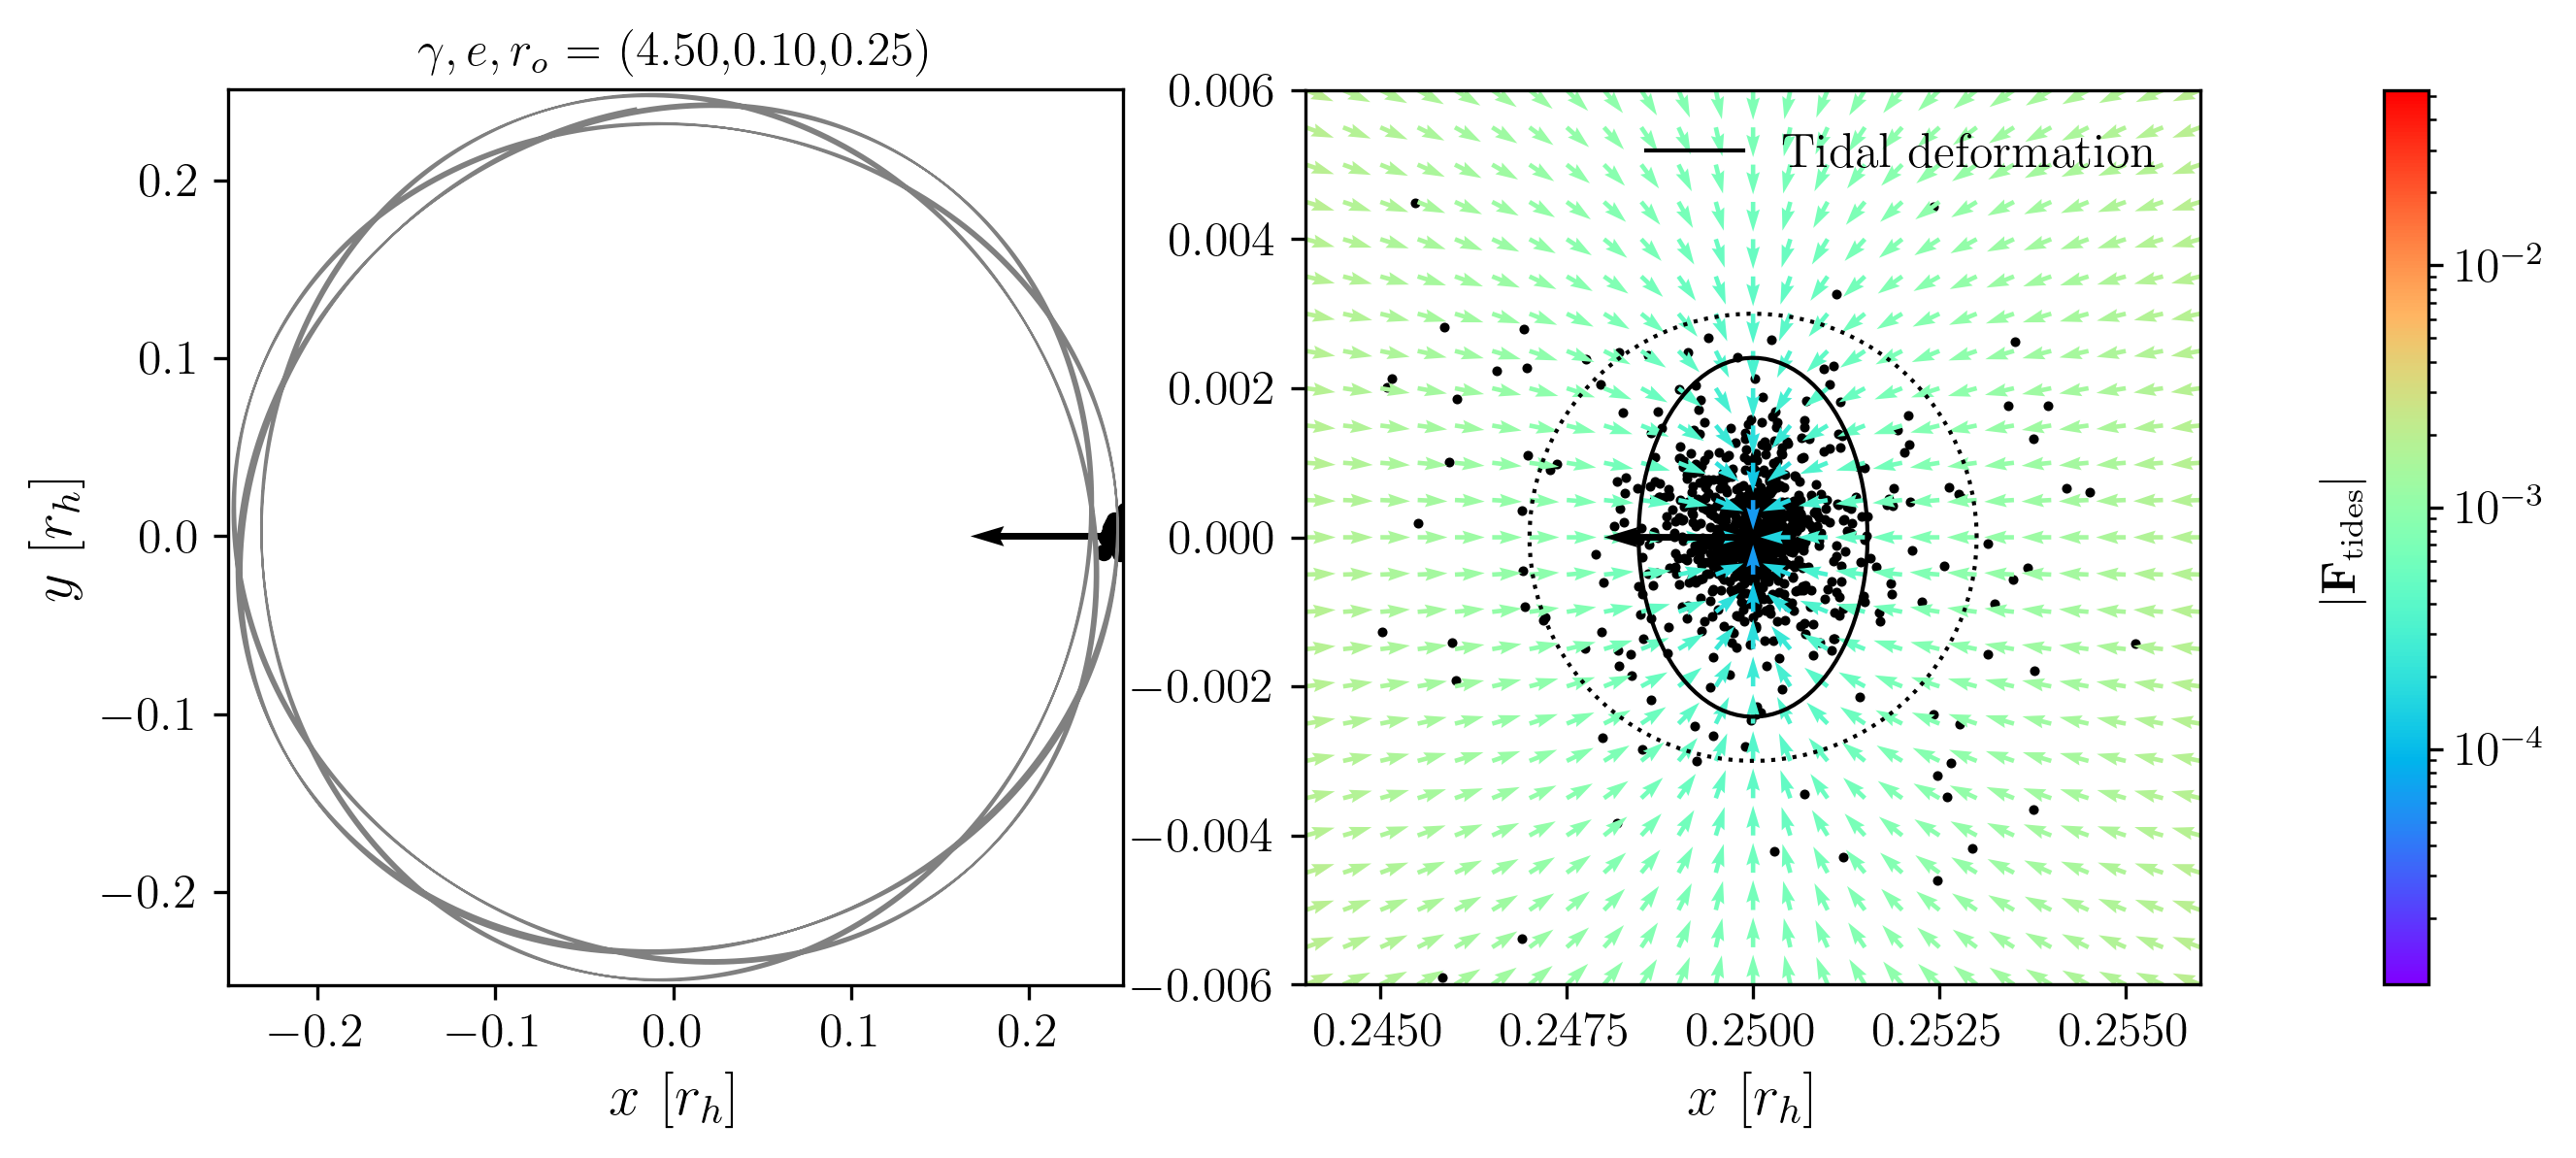
\includegraphics[width=\linewidth]{images/martos_tidal_field_450_10_25.png}
                \caption[Tidal forces from the Dark Matter halo in the inner galaxy]{The plots show two low-resolution streams (N = 1000) created by dissolving a Plummer sphere in the Allen-Santillan halo potential. The units are scaled to the halo's characteristic radius. Gamma is the mass exponent and is the sole variable between the two simulations. The panels on the left show the orbit in gray and the stars in black. The black arrow points towards the center of the potential. The panels on the right show the tidal field, which is the tidal tensor evaluated at each position in space. The gray dotted circle is plotted with an arbitrary radius and is deformed by the tidal field into a black ellipse.}
                \label{fig:martos_tidal_field_small_r}
            \end{figure}

            \begin{figure}
                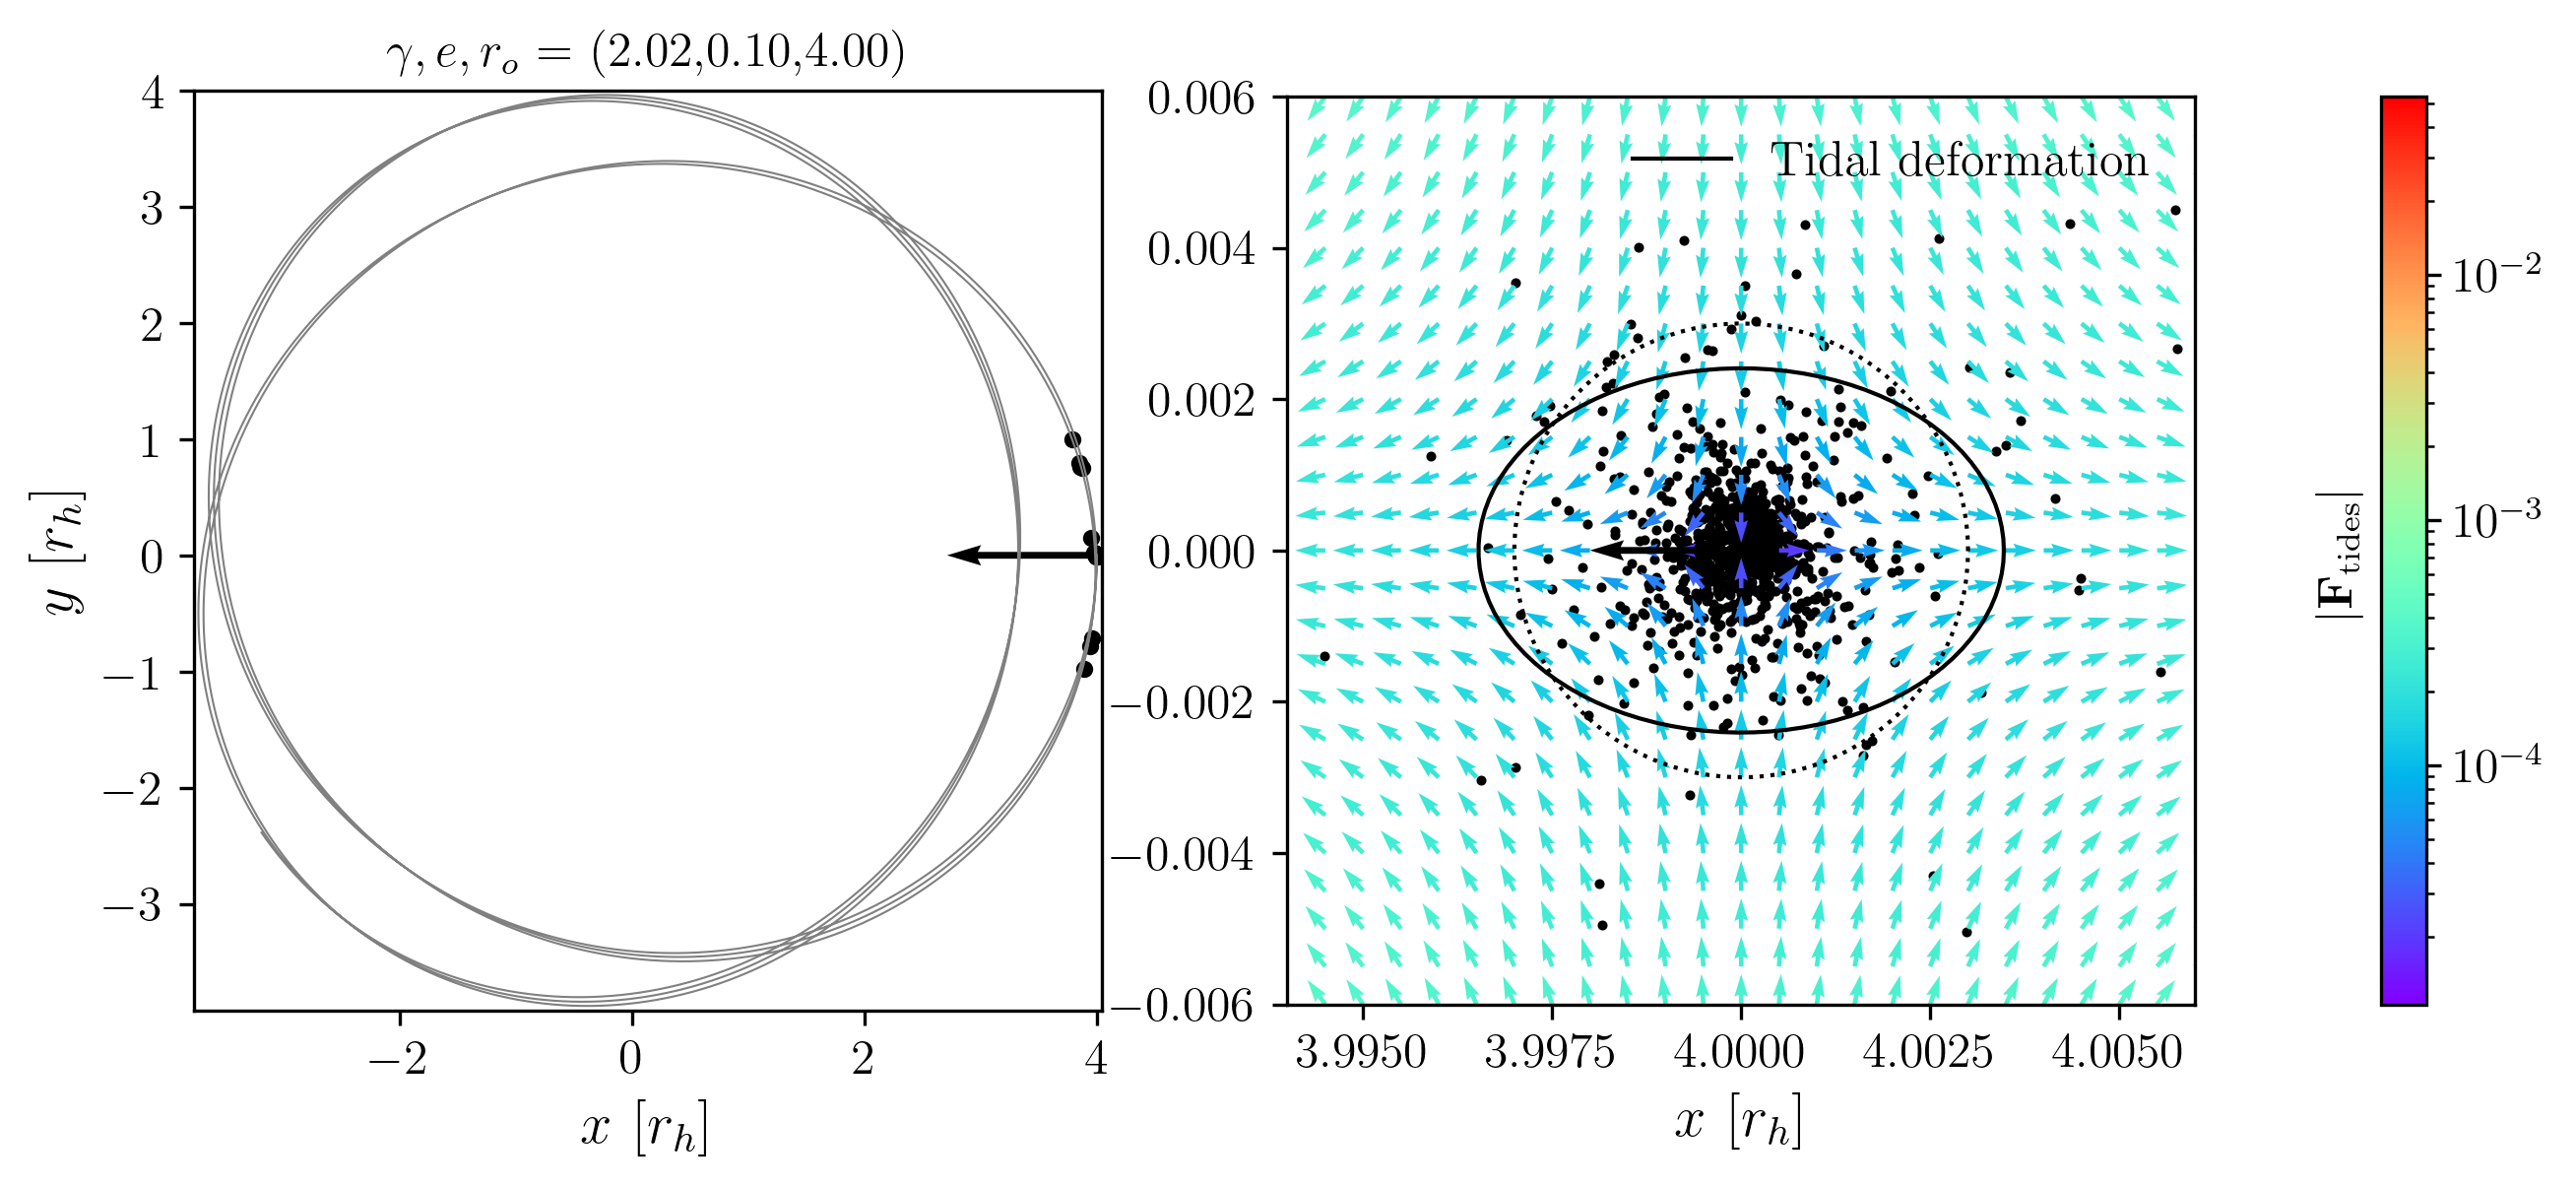
\includegraphics[width=\linewidth]{images/martos_tidal_field_202_10_400.png}
                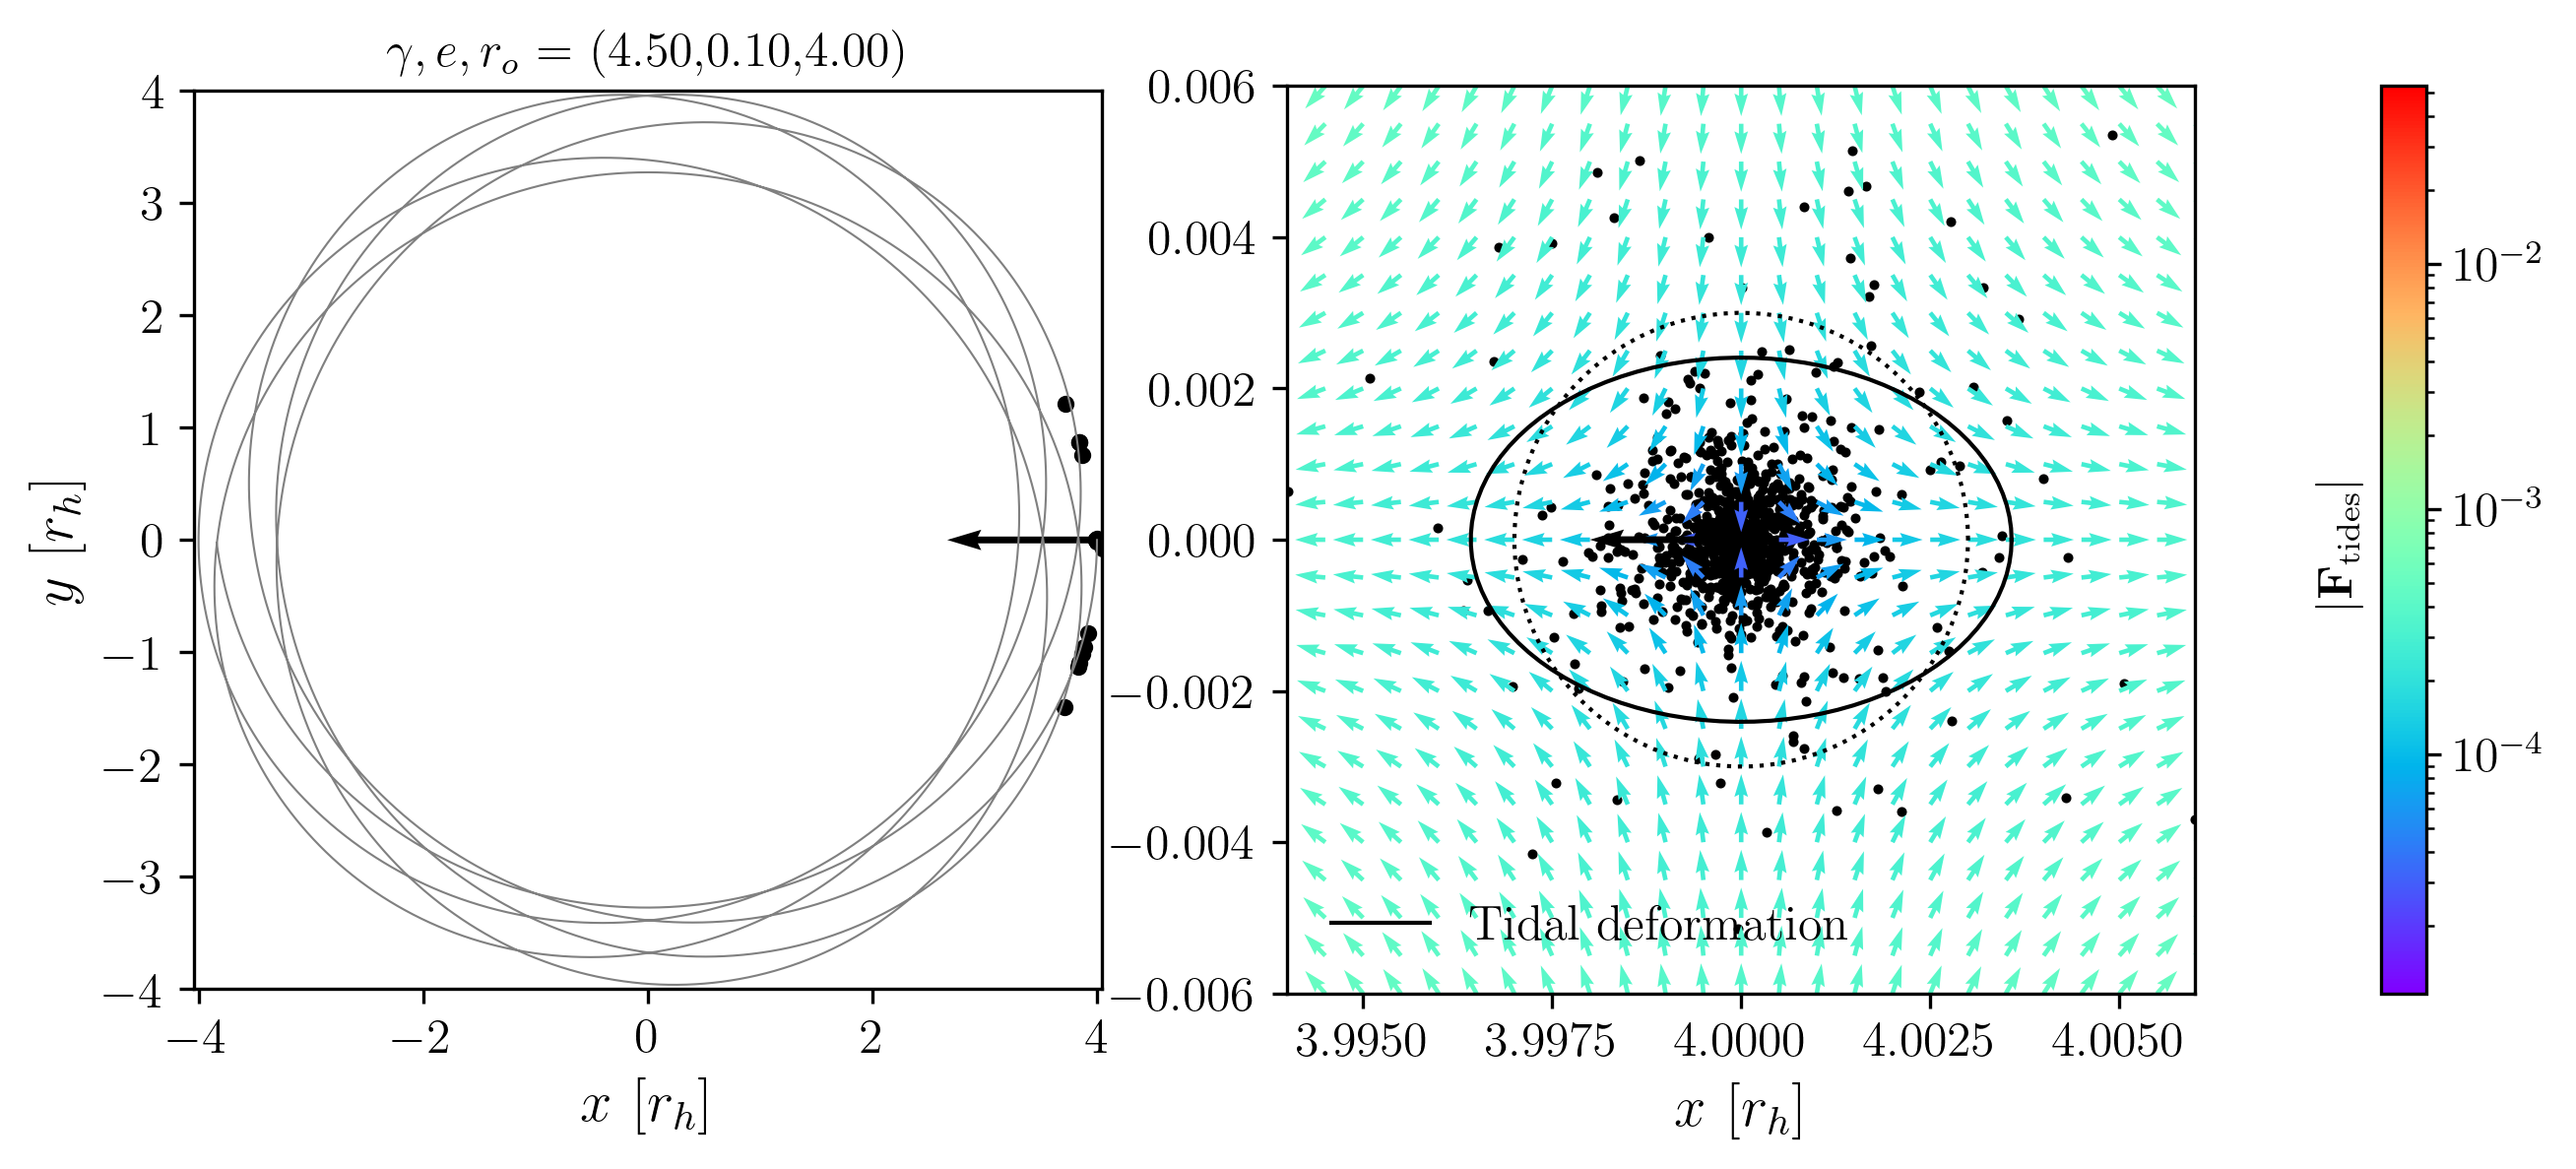
\includegraphics[width=\linewidth]{images/martos_tidal_field_450_10_400.png}
                \caption[Tidal forces from the Dark Matter halo in the outer galactic center]{The same experiment as Fig.~\ref{fig:martos_tidal_field_small_r}, but the cluster was placed at a larger distance of 4 $r_\textrm{halo}$, since we are beyond the characteristic radius, the tidal fields are the same, despite the different exponents $\gamma$.}
                \label{fig:martos_tidal_field_big_r}
            \end{figure}
            In the case of Fig.~\ref{fig:martos_tidal_field_big_r}, the tidal field returns to the typical situation where one axis is compressive and the other stretches. Notice how the deformations are similar in magnitude, while in the case of $\gamma=2.02$ for the top panel of Fig.~\ref{fig:martos_tidal_field_small_r}, the compression is stronger than the expansion. Both of these are different than the Keplerian tidal deformation where the stronger deformation is stretching and whose axis is parallel to the position vector. 

    \subsection{The Distribution of Escaped Stars}\label{sec:phaseMixing}
        Tidal forces cause stars to escape from the Lagrange points of the globular cluster. As we have seen, these forces can be compressive—pushing stars toward the cluster—or stretching—pulling them away, and specifically toward the Lagrange points. The stretching component is significantly amplified during pericenter passages, causing many stars to escape in bursts.

        This process does not fling stars into intergalactic space. Rather, the Galactic tidal field is typically weak compared to the cluster's own gravitational pull, and escaping stars gain just enough energy to leave the cluster. As a result, they are still on very similar orbits to the clusters once they escape.

        But once stars escape, why do they form coherent stellar streams? And do they do anything else? To answer this, I must first introduce the concept of \textit{phase mixing}. This naturally leads us to discuss the range of possible orbits a globular cluster can follow, given observational uncertainties. I'll cover this fully before returning to the topic of stellar streams, which will be much easier to understand once this groundwork is in place.
        
        \textit{Phase mixing} is a direct consequence of Liouville theorem, which follows from the collisionless Boltzmann equation. Liouville's theorem states that the infinitesimal volume element in phase space, \( d\mathbf{p}\,d\mathbf{q} \), is preserved under Hamiltonian evolution. In other words, the phase-space density \( f(\mathbf{q}, \mathbf{p}, t) \) remains constant along a particle's trajectory.

        To visualize this, instead of considering a single infinitesimal element, imagine a small cloud of initial conditions centered around \((\mathbf{q}_0, \mathbf{p}_0)\), with spread \(\sigma_q\) and \(\sigma_p\). While the total 6D volume of this cloud, \(\sigma_q^3 \sigma_p^3\), remains constant, differences in momentum cause the particles to move through phase space at different rates. Particles with higher momenta advance more quickly, while those with lower momenta lag behind. This leads to the cloud stretching and dispersing, even as its total volume is conserved. Since solutions to Hamilton's equations are unique, this dispersion reflects how nearby trajectories gradually diverge and spread over the available phase space—a process we call phase mixing.

        We can estimate the timescale for this spreading by considering how long it takes for orbits with slightly different energies to drift apart in phase. For example, in a Keplerian potential, the orbital period is given by
        \begin{equation}
            T^2 = \frac{4\pi^2 a^3}{GM},
        \end{equation}
        which depends on the semi-major axis, and thus on energy. In general, orbits in non-Keplerian potentials are not closed; particles precess and eventually fill out invariant tori in phase space. A characteristic timescale for this process can be estimated by dimensional analysis as
        \begin{equation}
            T_\mathrm{char} = C \frac{GM}{E^{3/2}},
        \end{equation}
        where \(C\) is a constant and \(E\) is the specific orbital energy.

        Consider now two nearby particles with energies $E - \Delta E$ and $ E + \Delta E $. Their orbital frequencies differ by:
        \begin{equation}
            \Delta f = \frac{1}{T( E - \Delta E)} - \frac{1}{T(E + \Delta E)}.
        \end{equation}
        The time required for the faster particle to lap the slower one in phase is the \textit{phase mixing time}, which is the inverse of the difference $2\pi / \Delta f$ and is given by:
        \begin{equation}
            T_\mathrm{mix} = \frac{2\pi}{\Delta f} = \frac{2\pi T_1 T_2}{T_2 - T_1}.
        \end{equation}
        For small energy differences \( \Delta E << E \), we can expand the period in a Taylor series to first order. This leads to:
        \begin{equation}
            T_\mathrm{mix} \approx T_\mathrm{char} \cdot 2\pi \left( \frac{E}{3 \Delta E} \right),
            \label{EQ:phase_mixing}
        \end{equation}
        Thus, the phase mixing time grows inversely with the relative energy spread in the population.
        \subsubsection{Orbital drift}
            The first manifestation of phase mixing is the growth of uncertainty in orbital solutions for globular clusters over time. This originates from the initial spread in orbital energies caused by observational uncertainties. In Fig.\ref{fig:phase_mixing_palomar_5_orbital_solutions}, I present an example based on Palomar~5, for which I compute 50 orbital solutions in our potential model. These initial conditions are sampled according to the uncertainties reported in the Baumgardt catalog. The figure shows that while the orbital solutions remain broadly similar, the lower-energy orbits progress through phase space more rapidly. In the bottom panel, the rightmost side includes overplotted dots indicating the final $(t, z)$ coordinates of each solution, illustrating that they span nearly the full range of $z$ values allowed by the initial conditions. In essence, once the integration time exceeds the phase-mixing timescale, any individual solution becomes speculative: the system could plausibly occupy any location in phase space permitted by the initial conditions.
            \begin{figure}
                \centering
                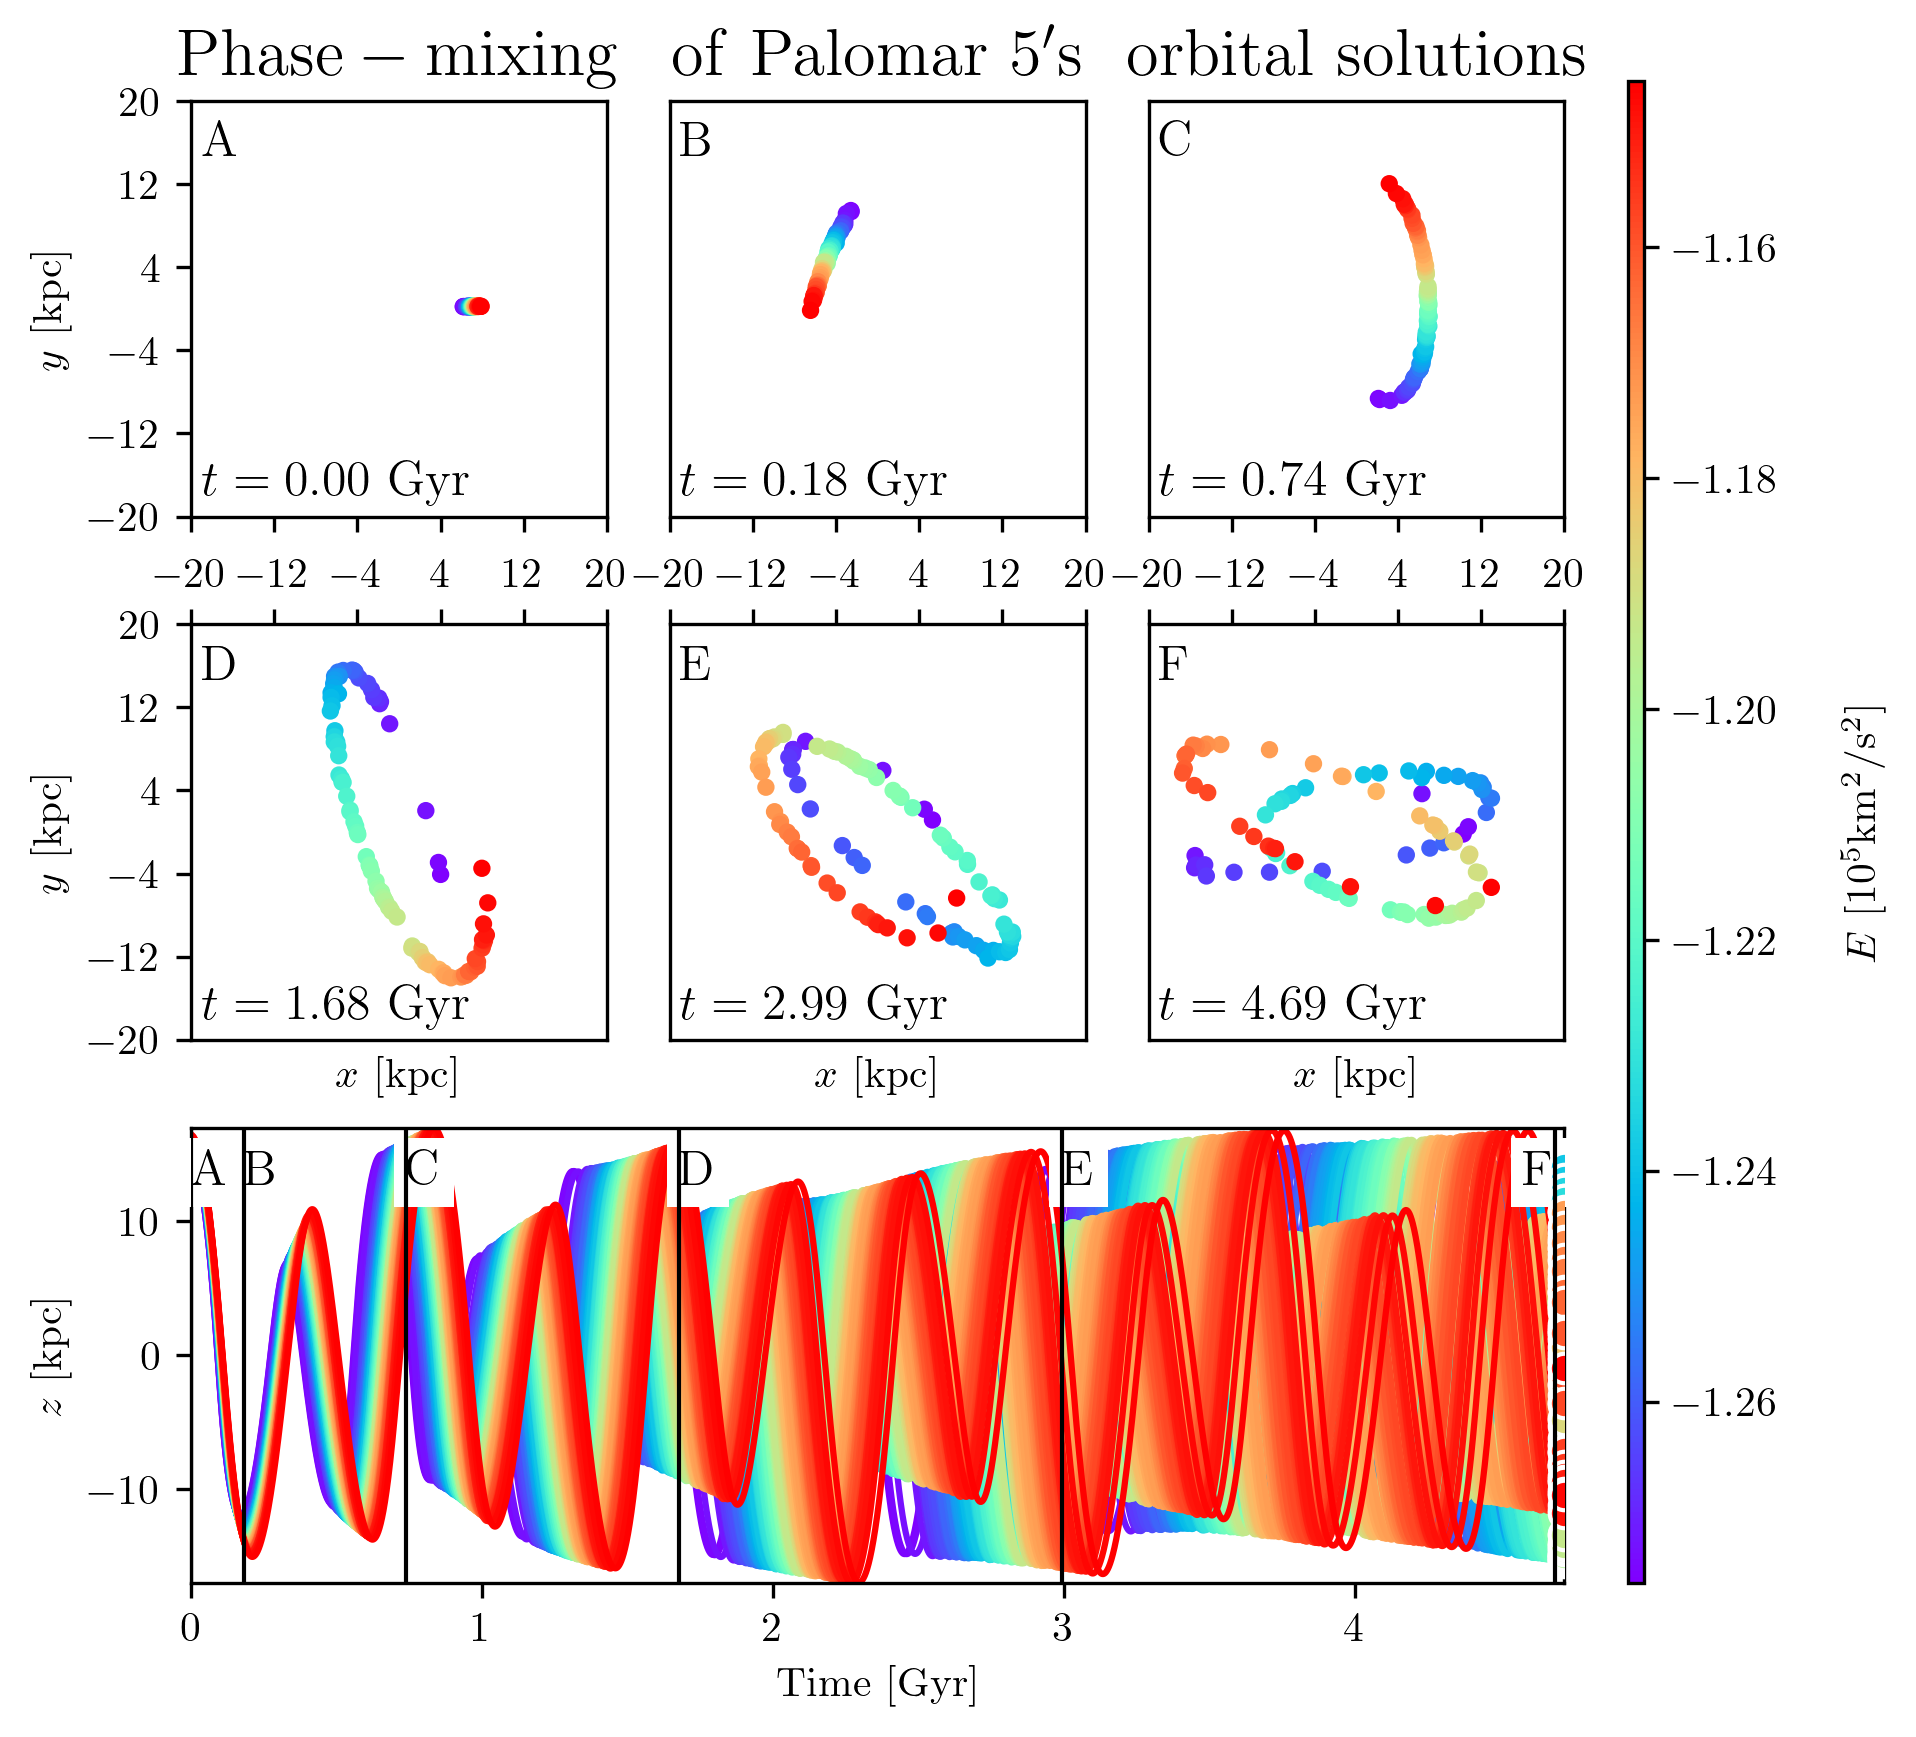
\includegraphics[width=\linewidth]{images/phase_mixing_palomar_5_orbital_solutions.png}
                \caption[Phase-mixing of Palomar 5's orbital solutions]{Phase mixing of Palomar~5's orbital solutions in the bulge-less model potential of \citet{2017A&A...598A..66P}. We sample 50 different initial conditions based on the observational uncertainties in distance, radial velocity, and proper motions. Each orbital solution is color-coded by its initial total orbital energy $E$. The top six panels show snapshots of the positions in the $xy$-plane of the orbital solutions at different times. The bottom panel shows the evolution of the $z$ coordinate as a function of time. Black vertical bars mark the timestamps corresponding to the snapshots in the top panels, which are labeled with matching alphabetical identifiers.}
                \label{fig:phase_mixing_palomar_5_orbital_solutions}
            \end{figure}
            By inspecting Eq.\ref{EQ:phase_mixing}, we note that if the phase-mixing time is normalized by the characteristic orbital time, the resulting dimensionless mixing time is inversely proportional to the uncertainty in orbital energy. This relationship is general and holds for all orbits, regardless of their periods. However, it is still illustrative to examine this behavior in the context of the globular cluster catalog. In Fig.\ref{fig:phase_mixing_orbital_errors_sample}, I present the phase-mixing times for all Galactic globular clusters, based on current uncertainties from the Gaia DR3 catalog. The top panel shows the distribution for all 165 clusters. The bottom panels highlight the mixing behavior in cylindrical radius for a selection of statistically representative clusters: Gran~1, which has the shortest mixing time; Gran~5, the median case; NGC~6752, whose mixing time is closest to the mean; and NGC~2419, which has the longest mixing time.

            It is important to emphasize that these estimates are highly model-dependent. In some cases, the models predict phase-mixing timescales exceeding the age of the Universe. Unsurprisingly, the phase-mixing time correlates with the orbital period, which itself is related to the cluster's distance from the Galactic center. At large Galactocentric distances, the gravitational potential of the Milky Way becomes increasingly uncertain, as observational constraints on the Galactic mass distribution are weaker---See Fig.~\ref{fig:vasiliev_2021_EDR3_GCS_FIG_10} \citep{2021MNRAS.505.5978V}. Therefore, these extreme mixing times should not be interpreted as implying that we can predict the phase-space location of certain clusters with high confidence over cosmological timescales. 
            \begin{figure}
                \centering
                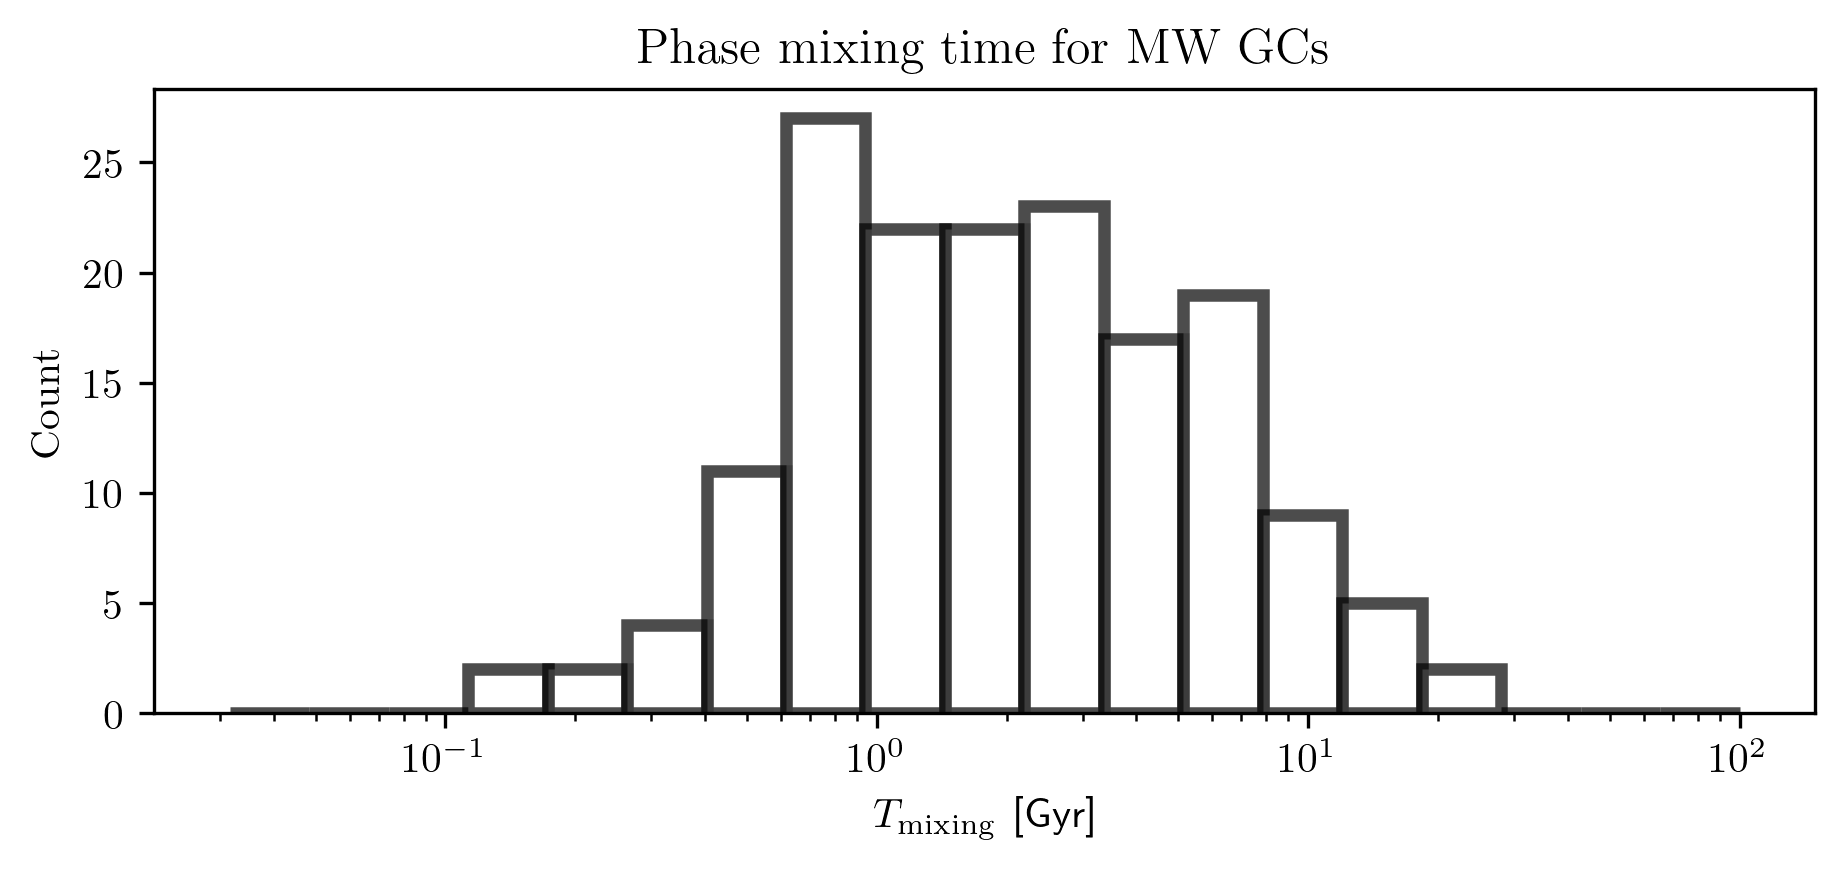
\includegraphics[width=.75\linewidth]{images/phase_mixing_time_histogram_MWGCS.png}
                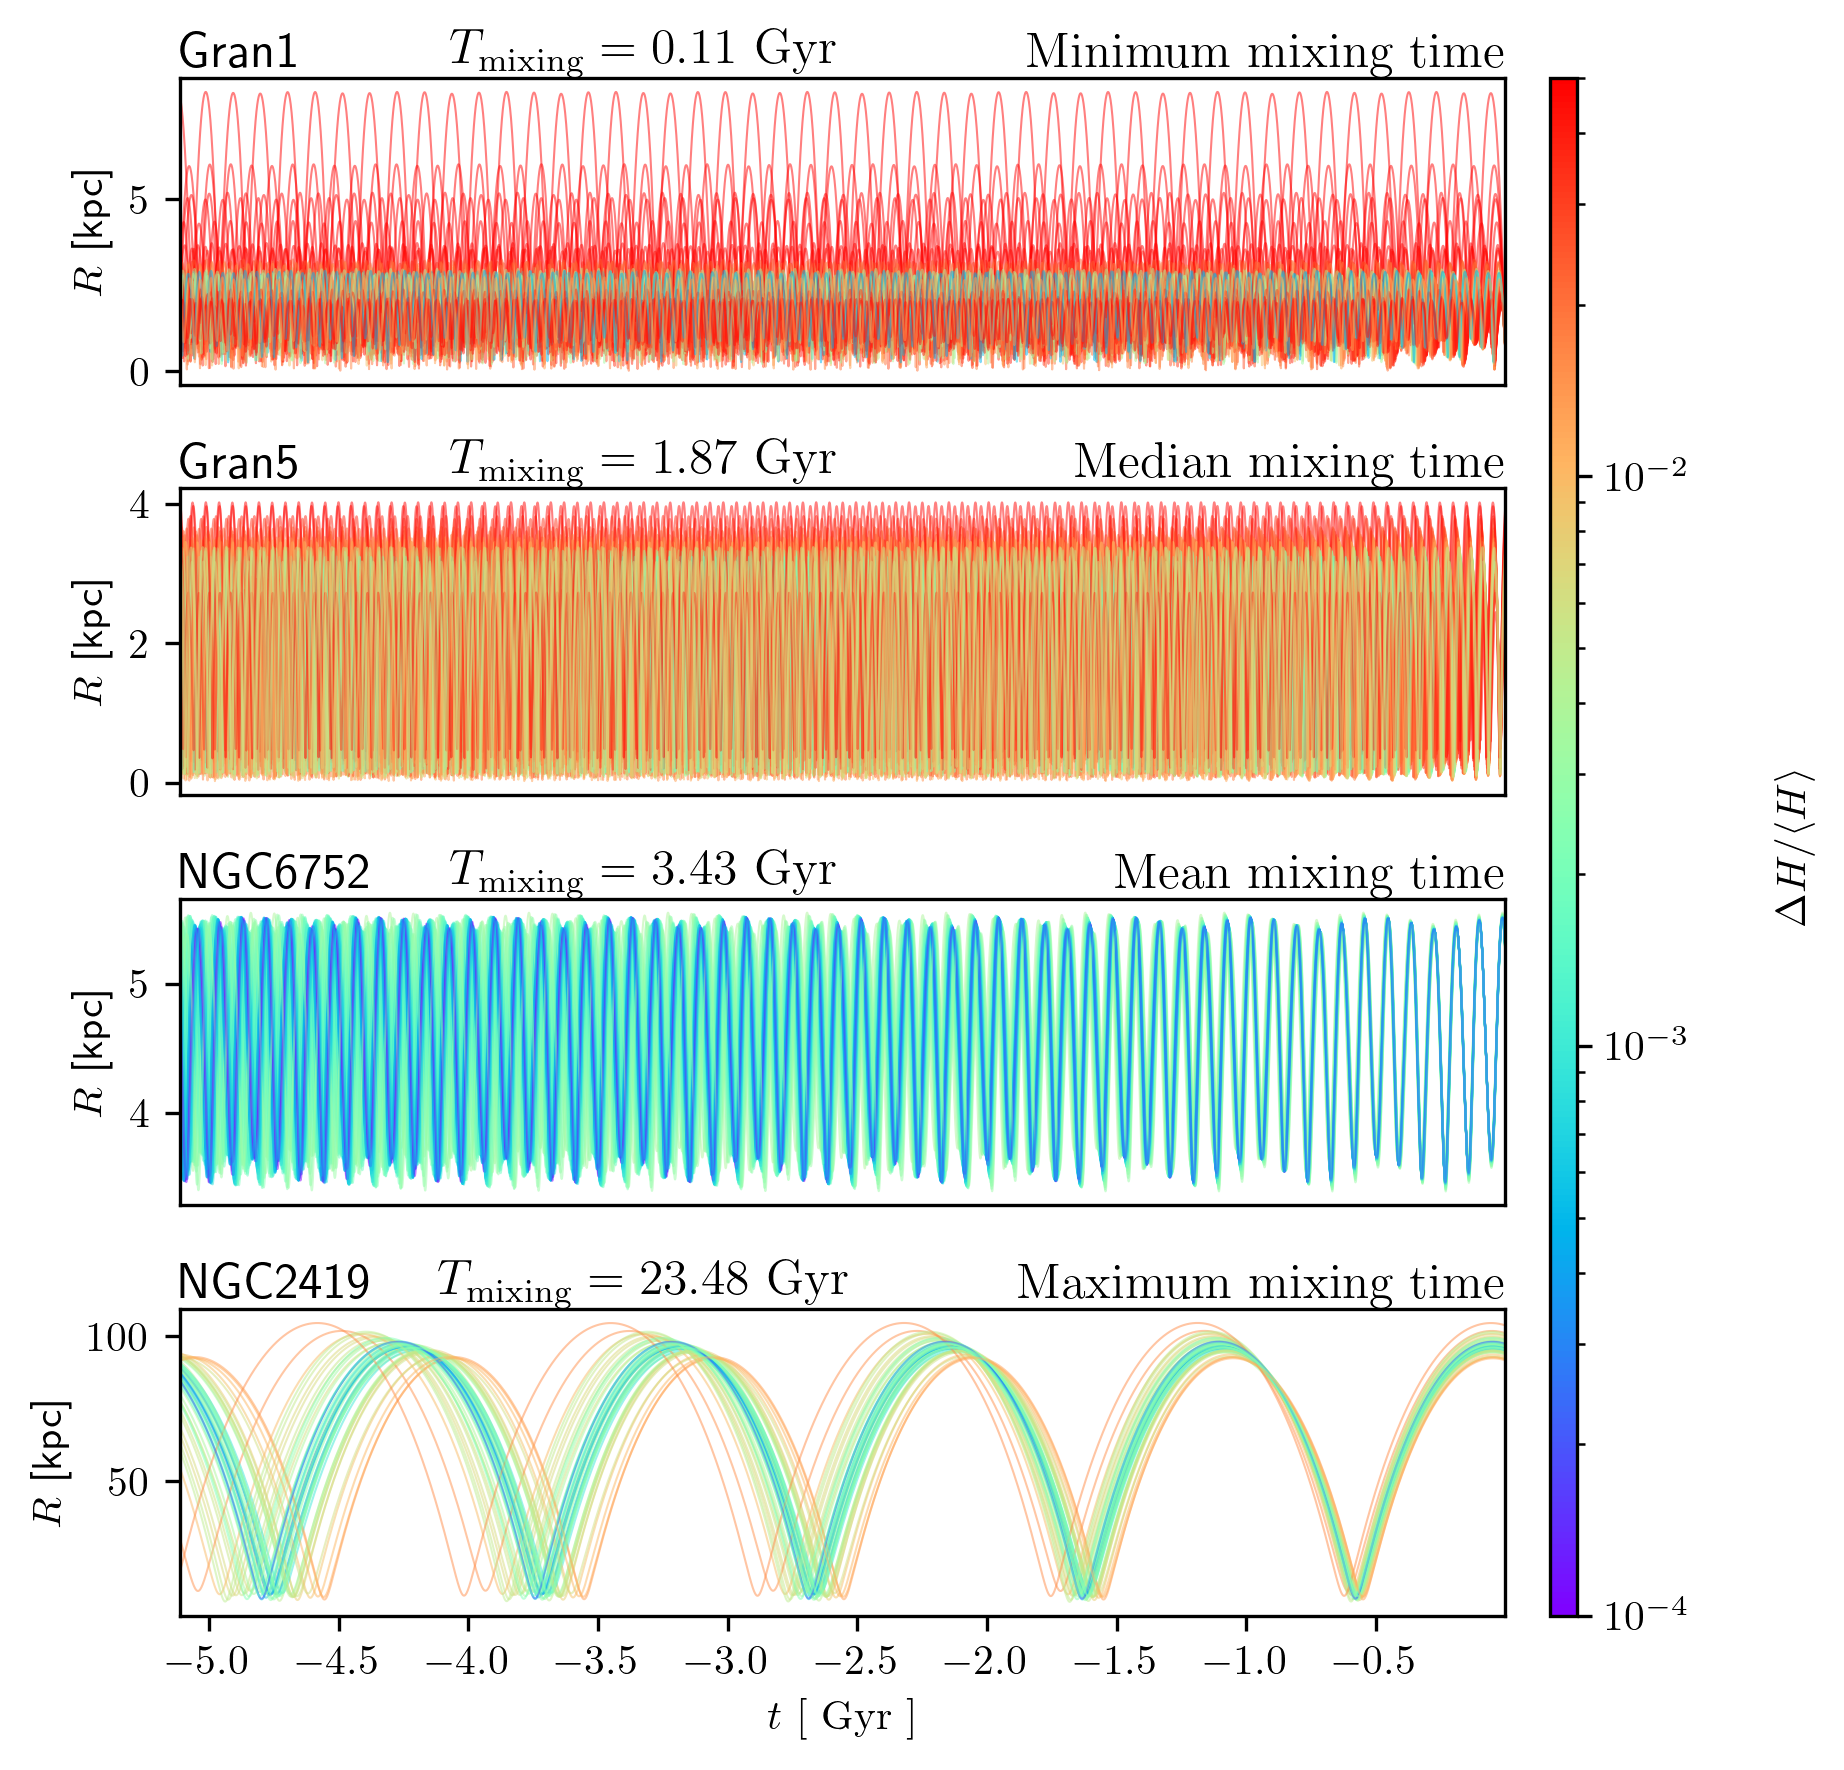
\includegraphics[width=\linewidth]{images/phase_mixing_orbital_errors_sample.png}
                \caption[Phase mixing time of the globular cluster catalog]{The top panel shows the distribution of phase-mixing times for globular clusters, computed using Eq.~\ref{EQ:phase_mixing}. The following four rows illustrate the phase-mixing behavior for four selected clusters over the time range considered in this experiment. Orbital solutions are color-coded by their normalized deviation from the mean orbital energy.}
                \label{fig:phase_mixing_orbital_errors_sample}
            \end{figure}
            It is also informative to examine how uncertainties in orbital energy relate to uncertainties in the individual observables. In Fig.~\ref{fig:energy_sensitivity_analysis_MWGCS_to_distance_RV_mu}, I illustrate this with a simple calculation. The measurements of the globular clusters, along with their associated uncertainties, are reported in the ICRS. I sample the observables assuming Gaussian errors and transform the coordinates to the Galactocentric reference frame.
            \begin{figure}[p]
                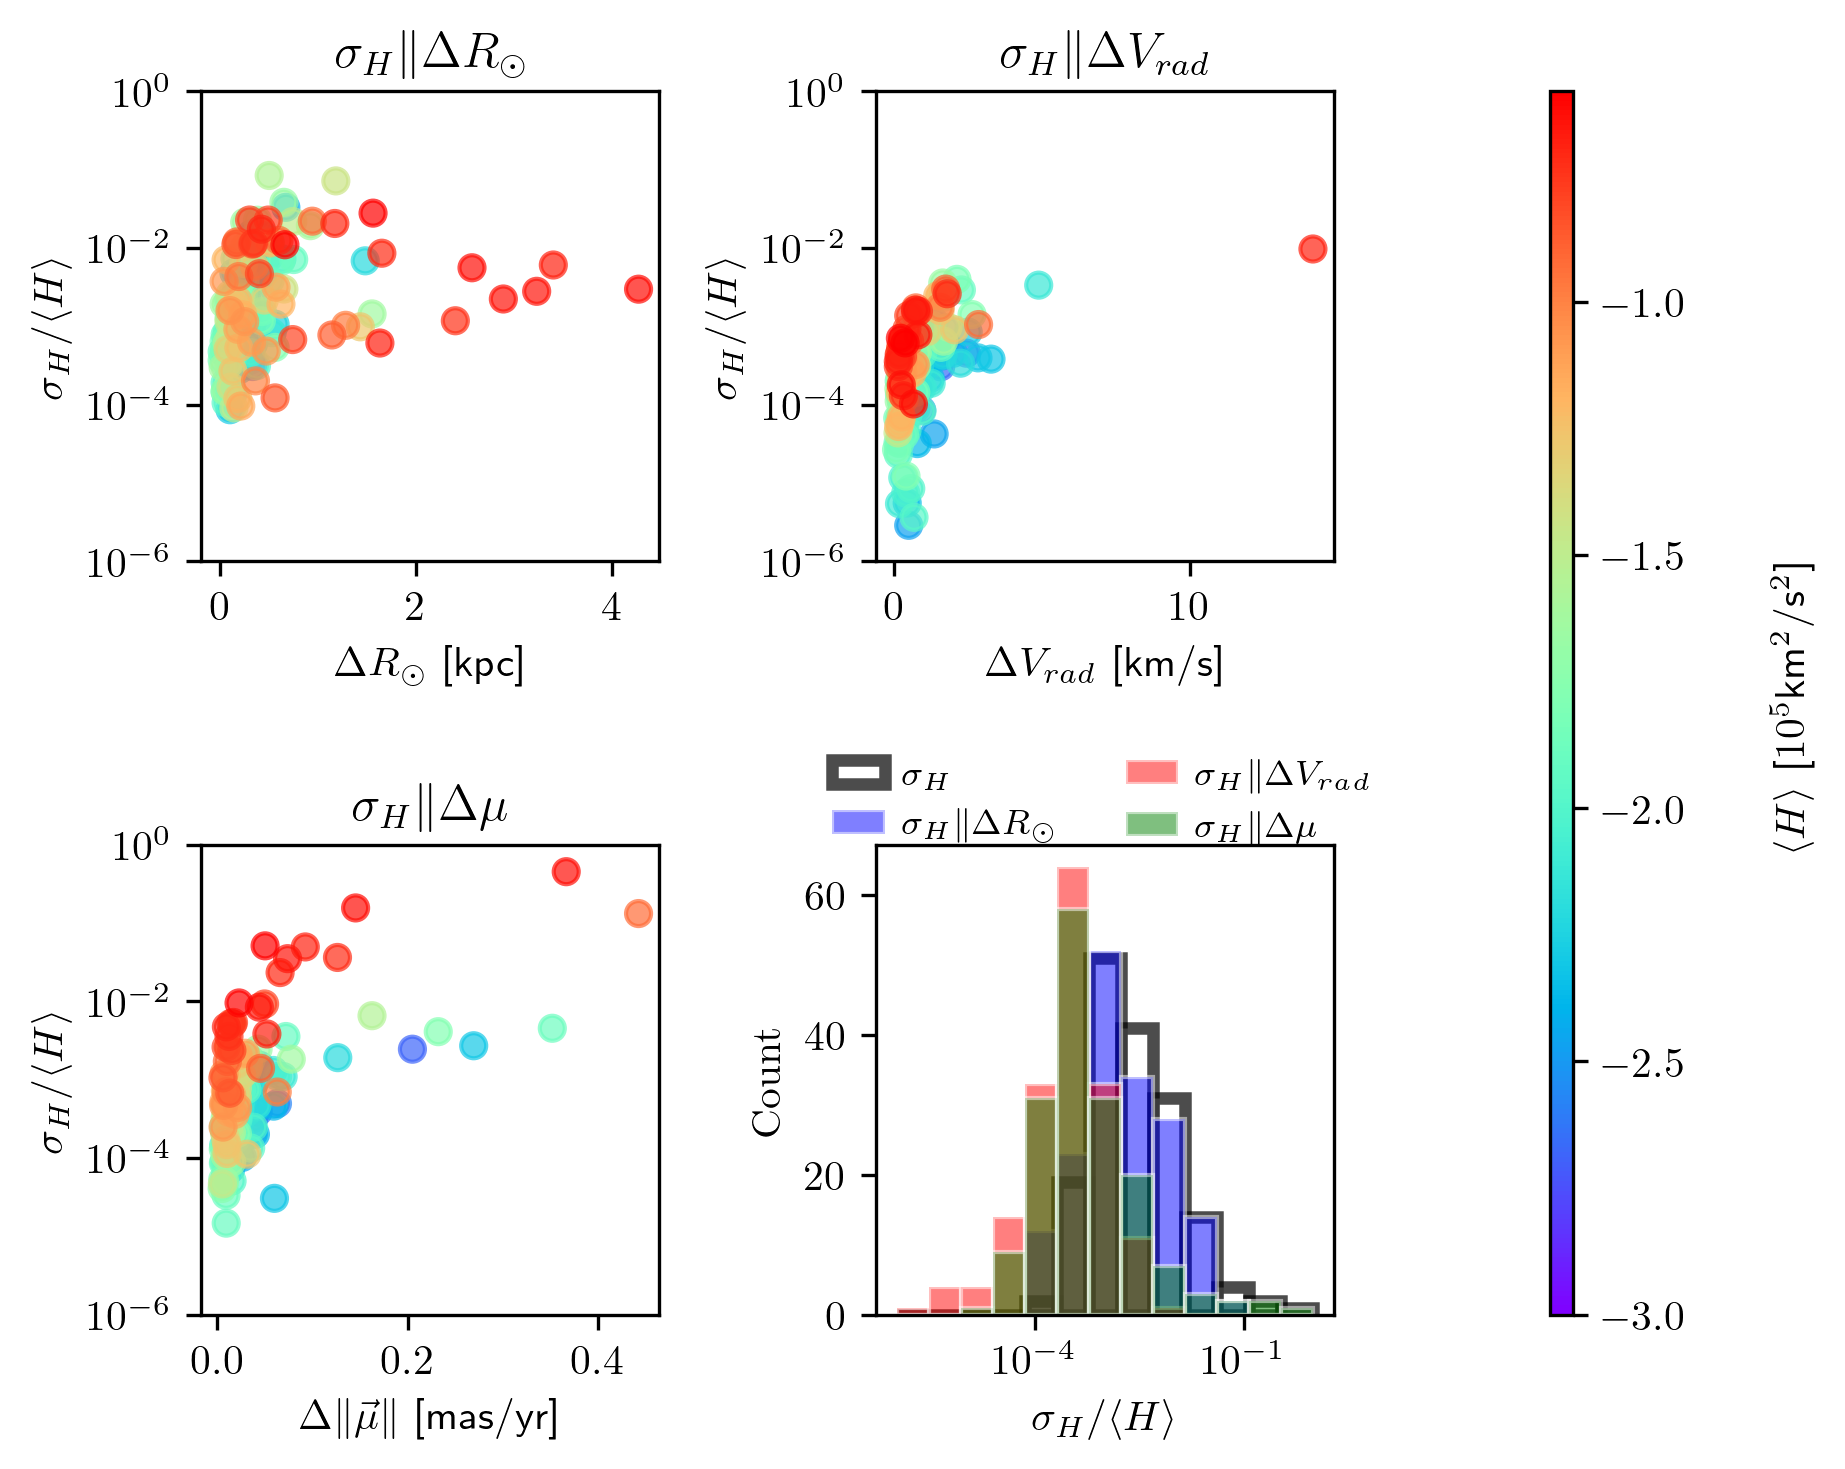
\includegraphics[width=\linewidth]{images/energy_sensitivity_analysis_MWGCS_to_errors.png}
                \caption[Uncertainty analysis of the globular cluster orbital energies]{An analysis on the spread in orbital energies of the globular cluster population for each of its reported uncertainties. Each panel finds the STD in the Hamiltonian given the uncertainties in the specific variable. So the top left allows the distances to vary but holds the proper motions and radial velocities constant. It is plotted against the distance. The clusters are color-coated by their mean energies.}
                \label{fig:energy_sensitivity_analysis_MWGCS_to_distance_RV_mu}
            \end{figure}
            In short, the phase-mixing time for a given set of orbital solutions and the uncertainty in the initial conditions can be interpreted as: ``how long until I have no idea where this cluster is?'' Beyond this timescale, the cluster's position has an equal probability of being anywhere in phase-space permitted by its integrals of motion. This concept will be important in Chapter~5, where we assess whether different possible orbits for the globular clusters could have brought them into contact with the Palomar~5 stream.
        \subsubsection{Mixing of globular cluster tidal debris}
            A cloud of points that starts tightly packed in phase space and gradually disperses provides a useful analogy for the evolution of tidally escaped stars from globular clusters into stellar streams. At first glance, Fig.~\ref{fig:phase_mixing_palomar_5_orbital_solutions} may appear to show the time evolution of a single stream, but it actually depicts different orbital solutions. The visual similarity highlights that both phenomena are governed by phase mixing.

            However, there is a key distinction. The divergence of orbital solutions is a direct consequence of Liouville's theorem: the particles are non-interacting and evolve independently in a fixed potential. In contrast, stars in globular clusters are bound by their mutual gravity, which slows down phase mixing. As a result, the cluster dissolves over a longer timescale than the idealized mixing time in Eq.~\ref{EQ:phase_mixing}. Still, phase mixing governs the long-term behavior of the unbound stars.

            Crucially, we do not need to model the entire cluster to study tidal debris as a phase-mixed population. For clusters with short mixing times relative to the simulation length, the escaped stars can explore the accessible phase space, even if the debris remains non-uniform and overdense near the cluster. This insight is central to the results presented in Chapter 4.

            This idea is evident in \citet{2024ApJ...976...54P}, who predict that many more stellar streams remain to be discovered in the Milky Way. They note that while about 170 globular clusters are known today, many others likely existed in the past but have since dissolved. Their tidal debris may now form stellar streams, many of which remain undetected. Indeed, most of the $\sim$90 known streams are unassociated with any surviving globular cluster \citep{2022ApJ...926..107M}, and only about 20 have confirmed associations \citep{2024ApJ...967...89I}.

            To estimate the full population of globular cluster streams, \citet{2024ApJ...976...54P} used the IllustrisTNG simulations \citep{2019ComAC...6....2N}, injecting globular clusters both formed in situ and accreted via dwarf galaxies following the prescriptions of \citet{2022MNRAS.514.4736C,2023MNRAS.522.5638C}. They then modeled the dissolution of these clusters and studied the resulting tidal debris. A panorama of their predicted streams is shown in Fig.~\ref{fig:perason-2024-fig}.

            \begin{figure}
                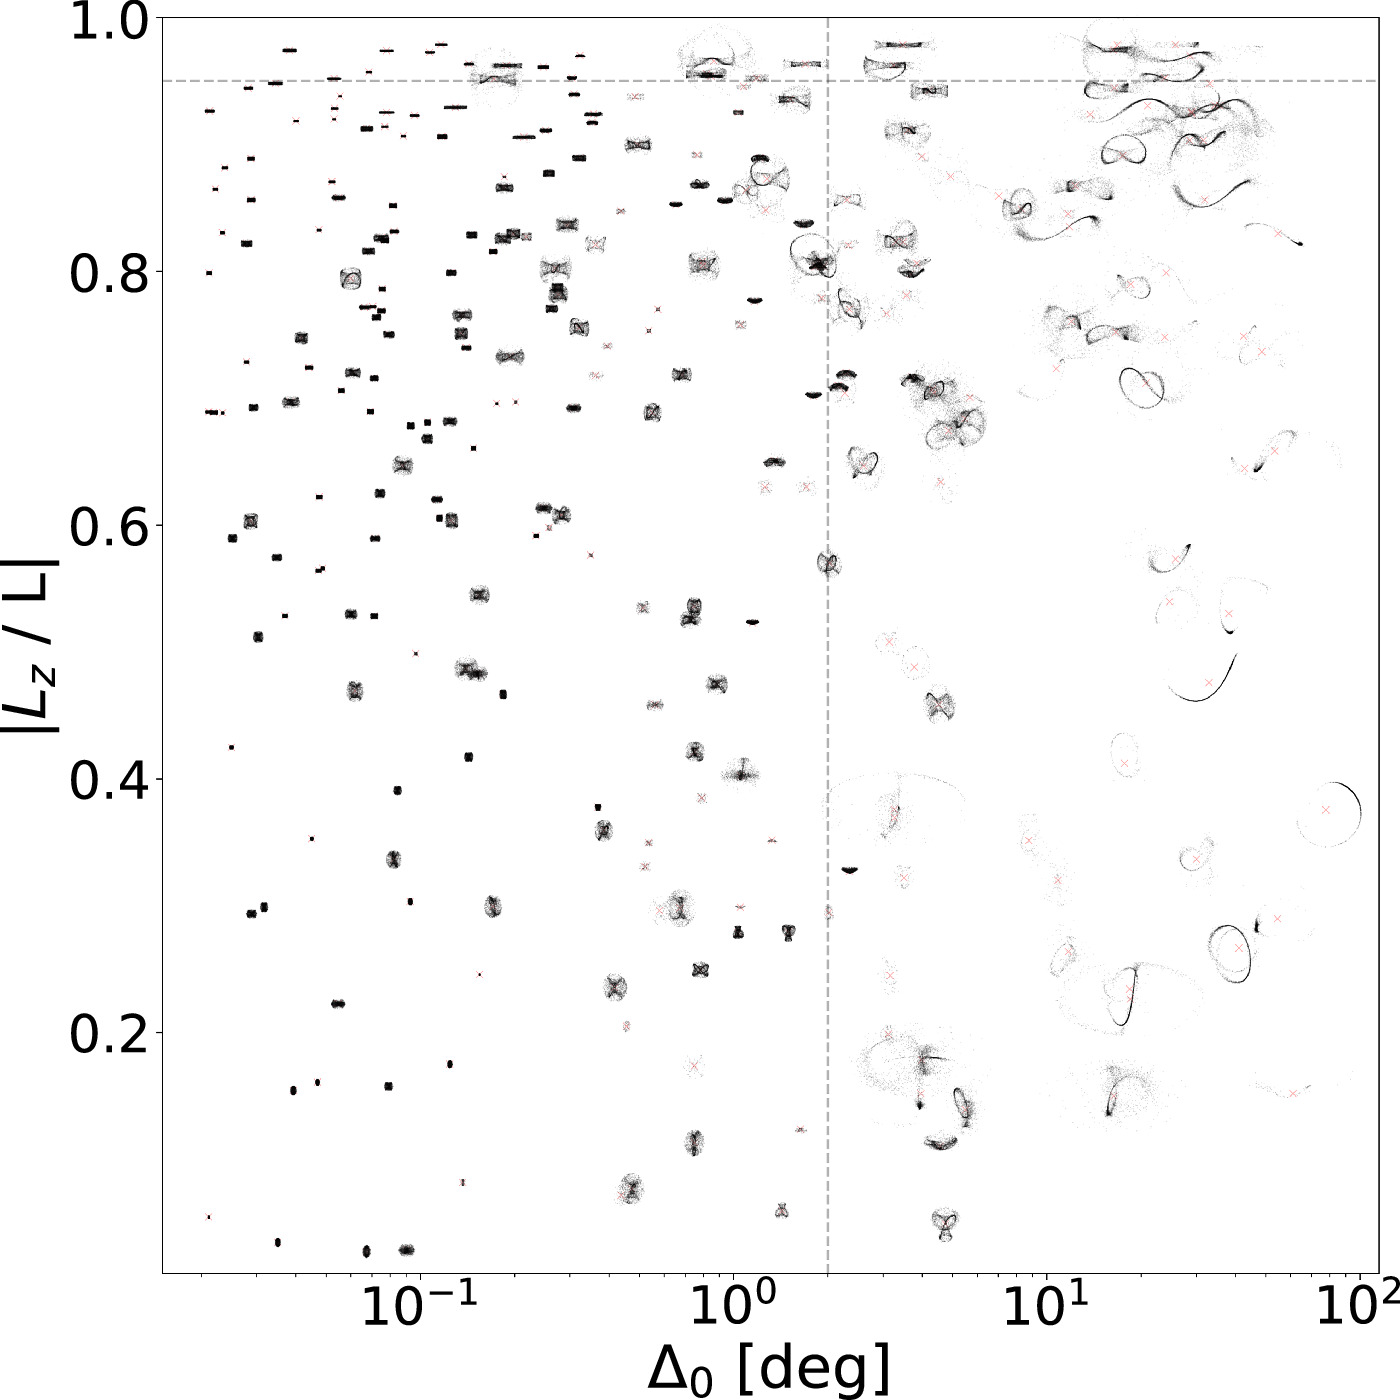
\includegraphics[width=\linewidth]{images/perason-2024-fig.jpg}
                \caption[Catalog of predict tidal debris of a theoretical globular cluster population in a Milky Way analog]{A catalog of predicted debris from a fully disrupted population of globular clusters in a Milky Way analog. The y-axis shows the normalized $z$-component of angular momentum (0 = polar, 1 = planar). The x-axis shows the distance of the stream's center of mass from the Galactic center. Each stream is plotted in Galactic coordinates and to scale. The bottom-right quadrant satisfies their ``streaminess'' criterion. Credit: Fig.~7 of \citet{2024ApJ...976...54P}.}
                \label{fig:perason-2024-fig}
            \end{figure}

            To assess stream detectability, \citet{2024ApJ...976...54P} introduced a ``streaminess'' criterion based on two metrics. One is the angular distance between a stream's center of mass and the Galactic center in Galactic coordinates:
            \[
            \Delta_0 = \sqrt{\mathrm{medn}(b)^2 + \mathrm{medn}(l)^2}.
            \]
            A small $\Delta_0$ indicates the debris is symmetrically distributed about the Galaxy, and thus fully phase-mixed.

            Remarkably, even such fully mixed debris can still be detected as co-moving groups \citep{2018MNRAS.477.4063M,2018MNRAS.478.3862M}. Although these stars appear spatially diffuse, they continue to follow similar orbits, merely offset in phase. A striking example is the \textit{Fimbulthul} stream, which has been linked to $\omega$~Centauri (NGC~5139), the most massive globular cluster and a suspected remnant of an accreted dwarf galaxy \citep{2000LIACo..35..619M,2010ApJ...722.1373J}. Our simulations in Chapter~4 predict that $\omega$~Centaur's debris should be fully phase-mixed and fail the ``streaminess'' criterion. Yet, \textit{Fimbulthul} aligns precisely with the cluster's predicted orbit and matches $N$-body expectations \citep{2021ApJ...914..123I}.

            This highlights an important point: even when tidal debris is diffuse and mixed, the underlying orbital coherence can still enable its detection as a stellar stream.

    \subsection{Massive objects colliding with stellar streams}
        Previously, we described how stars escape from globular clusters, and how the escaped stars can redistribute themselves within the Galaxy under the influence of its smooth gravitational field. However, other processes can affect the stream. Notably, massive objects in the Galactic field can pass nearby and perturb the orbits of some of these stars.

        For such an interaction, we may compute the change in a star-particle's momentum between before and after the encounter. We can simplify the scenario by assuming that the star-particle is initially at rest, and that the perturber (the subhalo) passes by with a minimum distance of approach $b$—the \emph{impact parameter}.

        Since both objects exert gravitational forces on each other, the star-particle will gain energy and begin to move, while the perturber will be slightly deflected and slow down. However, to simplify the calculation, we assume the perturber is unperturbed by the star-particle—i.e., it moves on a straight-line trajectory with constant speed $v$.

        In this \emph{impulse}-approximation, we compute the star-particle's change in momentum change by integrating the gravitational force over time of the interaction. Gravity is always attractive: the perturber pulls the star-particles particle to the left before the closest approach and to the right afterward. If the trajectory is symmetric and unperturbed, the components of the force parallel to the motion cancel out. Thus, the net momentum transfer is perpendicular to the motion of the perturber.

        Assume the perturber moves along the $x$-axis with impact parameter $b$, and the star-particles lies at the origin. Then the net force acts in the $+y$ direction. The gravitational force scales as $1/d^2$, so for distances $d >> b$, the force becomes negligible. We can then approximate the force as roughly constant over a short time interval during the closest approach.

        We estimate the duration of the interaction as the time it takes the perturber to travel a distance $2b$ (from $x = -b$ to $x = +b$), giving $\Delta t = 2b/v$. Assuming a constant perpendicular force $F_\perp \approx GMm/b^2$, the change in momentum is:
        \begin{eqnarray}
        m\,\delta v_y &=& \int F_\perp \, dt \\
                    &\approx& F_\perp \cdot \Delta t \\
                    &=& \frac{GMm}{b^2} \cdot \frac{2b}{v}
        \end{eqnarray}
        Dividing both sides by $m$, the change in velocity is:
        \begin{equation}\label{eq:delta_v_impulse_approx}
        \delta v_y = \frac{2GM}{b v}
        \end{equation}
        It is interesting to note that this result is inversely proportional to the velocity of the perturber. This behavior contrasts with contact collisions, where a higher speed typically results in a greater momentum transfer. In gravitational encounters, a faster flyby leads to a shorter interaction time and thus less momentum exchange.
        \subsubsection{Gap formation and evolution}
            Gaps in stellar streams are underdensities that appear after encounters with dark matter subhalos or -- as we will show in Chapter~5 -- globular clusters. These can be understood as resulting from collisions. However, modeling the interaction as one point mass hitting another is too simplistic. What happens when an extended object, like a subhalo, interacts with a continuous stellar stream? Before delving into the technical details, it is worth clarifying a misconception---one that I myself held when first approaching this problem. Encounters between stellar streams and perturbers are not violent collisions in which stars are physically ejected or stripped from the stream. Rather, the perturber imparts a small, localized change in velocity to nearby stars, subtly altering their orbital periods. Over time, these tiny shifts accumulate, causing stars to drift apart and gradually sculpting a visible underdensity: the gap. 
            
            To address this, we turn to the work of \citet{2015MNRAS.450.1136E}, who studied a simplified model: a stream with uniform density on a circular orbit. This idealized setup allows for an analytical treatment of the gap's formation and evolution. A gap can be characterized by two main quantities: its angular width, $\Delta \theta$, and the density contrast, $\rho_{\mathrm{peak}}/\rho_0$, between the overdensities at the gap's edges and the central underdensity.

            To understand how these evolve, the authors derived a parameterization of the change in velocity $\Delta \vec{v}$ for stars along the stream after a perturbation. This vector function depends on the position $y$ along the stream relative to the impact point and on several parameters describing the perturber and the impact geometry:
            \[
            \Delta \vec{v} = f(y \,|\, M, r_s, b, w_\parallel, w_\perp, \alpha),
            \]
            where $M$ is the impactor's mass, $r_s$ its scale radius, $b$ the impact parameter, $w_\parallel$ and $w_\perp$ the components of its velocity parallel and perpendicular to the stream, and $\alpha$ the angle between the impactor's trajectory and the $(x,z)$-axes.

            To set up the problem, a coordinate system is defined where the stream lies along the $y$-axis, and the impact occurs at $y=0$. Because the stream has spatial extent, the impactor's motion must be decomposed into parallel and perpendicular components with respect to the stream. Unlike the simpler point-mass approximation, here $\Delta \vec{v}$ generally has nonzero components in all directions. In particular, $\Delta v_y$ alters the speed along the stream, while $\Delta v_x$ and $\Delta v_z$ displace stars out of the stream's plane. $\Delta v_x$ or $\Delta v_z$ can be zero if the trajectory of the impactor is parallel to the $x$ axis or $z$ axis, respectively. 

            The expression for $\Delta v_y$ is:
            \[
            \Delta v_y\left(y\,|\, M, r_s, b, w_\parallel, w_\perp\right) = - \frac{2GM w_\perp^2 y}{w\left[\left(b^2 + r_s^2\right)w^2 + w_\perp^2 y^2\right]},
            \]
            which is an odd function of $y$, as expected for a gravitationally attractive force: stars ahead of the impact point ($y>0$) are slowed down, while those behind ($y<0$) are sped up.
            \begin{figure}
                \centering
                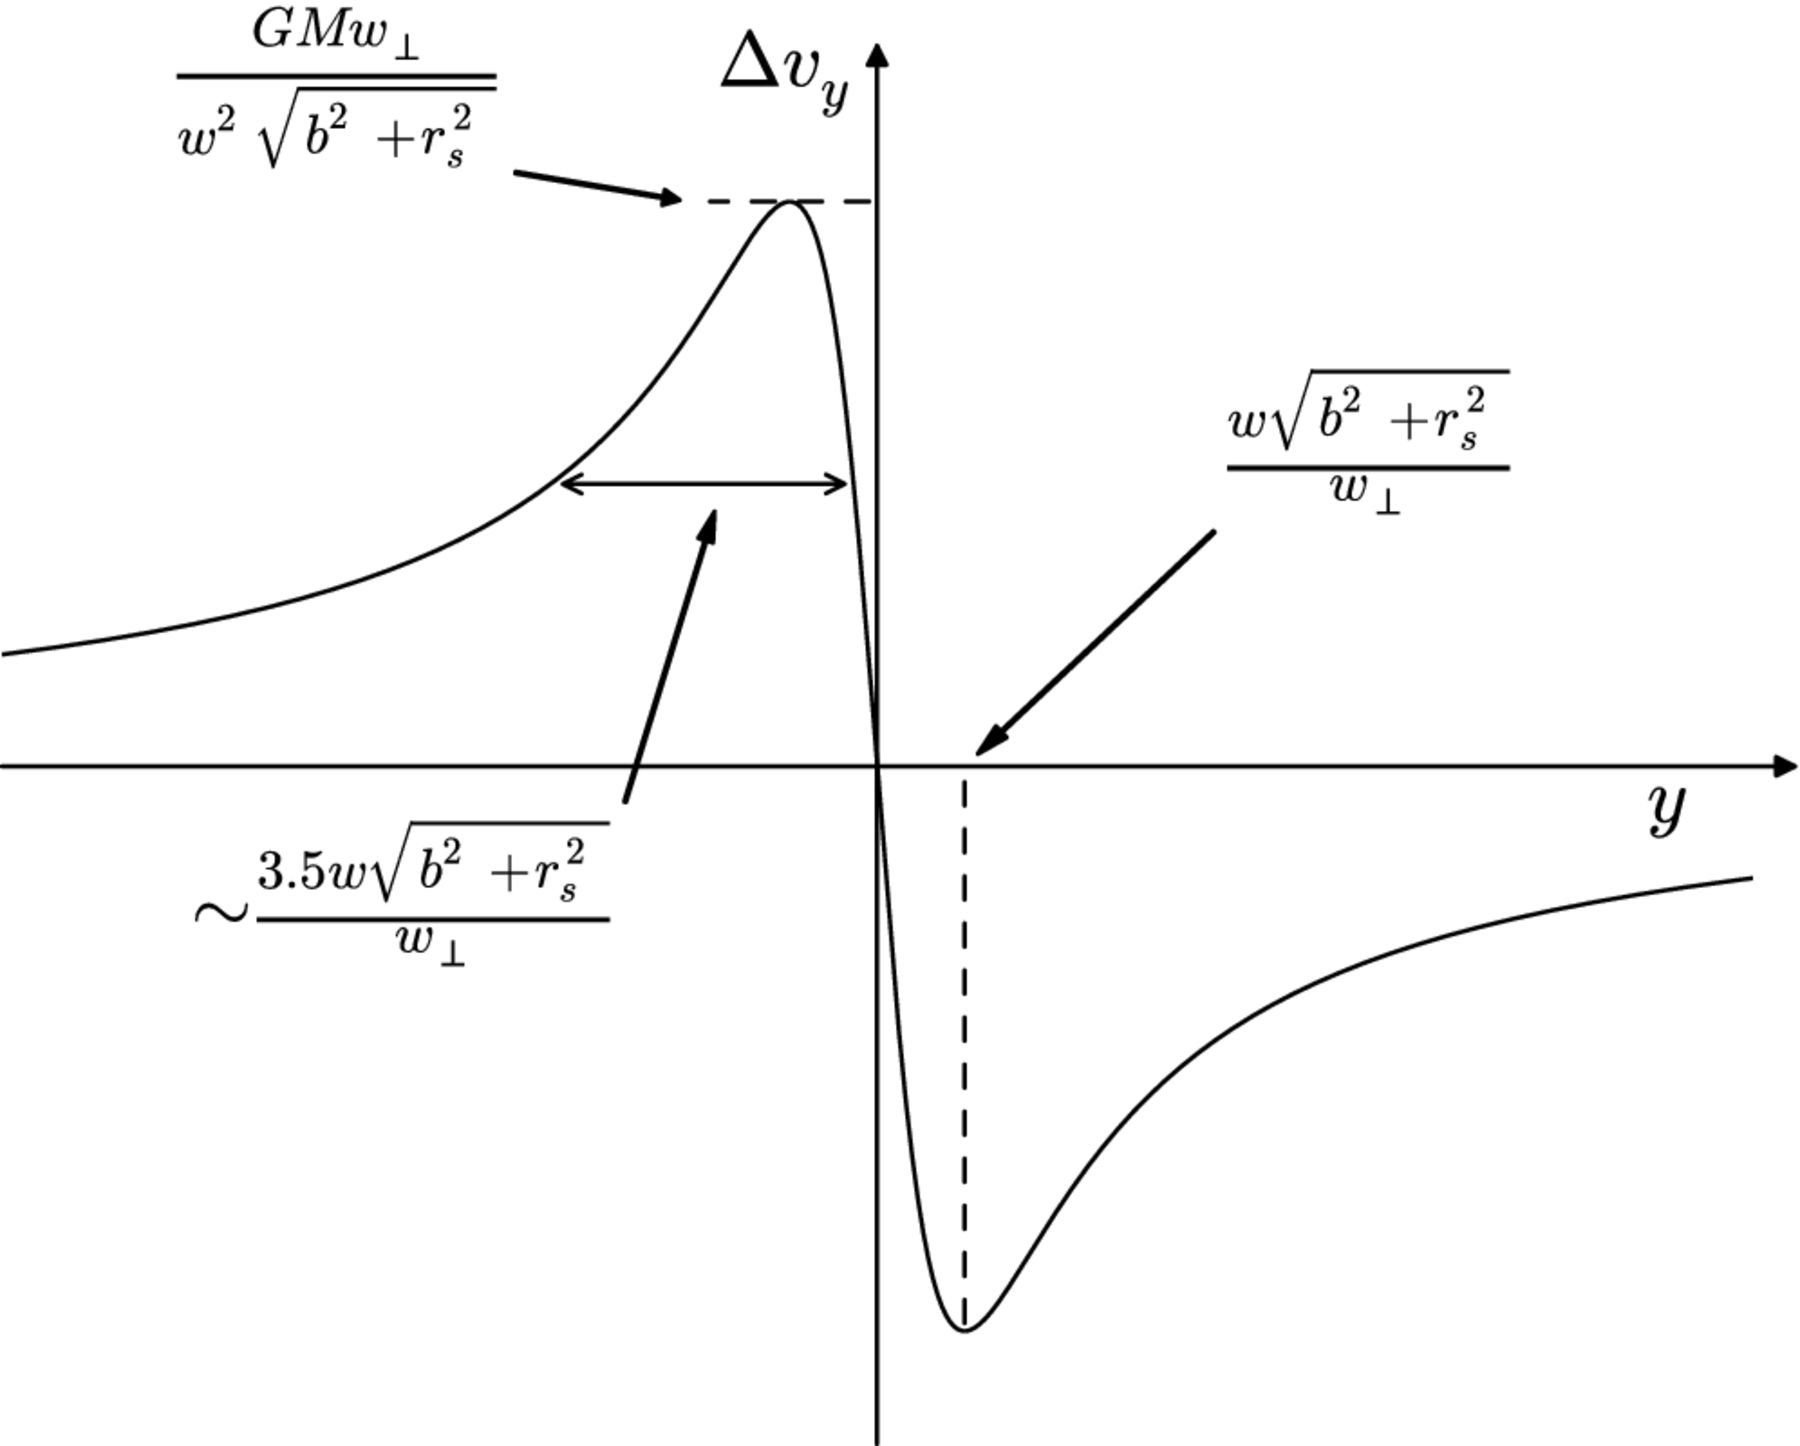
\includegraphics[width=0.5\linewidth]{images/erkal_et_al_2015_fig_3.png}
                \caption[Velocity kick on a stellar stream from a gravitational fly-by]{The change in velocity, $\Delta v_y$, of stars along the stream after an impact. The stream lies along the $y$-axis, with the point of impact at the origin. Key features are labeled: the maximum value of $\Delta v_y$, its location, and the full width at half maximum. Taken from Fig.~3 of \citet{2015MNRAS.450.1136E}.}
                \label{fig:erkal_2015_fig_3}
            \end{figure}

            Several assumptions underlie this formulation. First, the stream is approximated as a straight line, which requires the size of the impacted region to be much smaller than the orbital circumference. Second, the velocities of both the stream and the perturber are assumed constant, implying that the duration of the impact is much shorter than the system's orbital period. These assumptions also imply that the impactor must pass close to the stream and be compact relative to the stream's orbital radius.

            The authors then developed the time evolution of the stream's density following the impact. To study these, the authors employed three complementary approaches:
            \begin{enumerate}
                \item A numerical solution of a transcendental equation governing $\Delta \theta(t)$;
                \item A fully analytic solution for a low-order analytical approximation valid when the gap opening $\Delta \theta$ is still small;
                \item An $N$-body simulation of the full system.
            \end{enumerate}

            Together, these revealed three distinct phases of gap evolution:
            \begin{enumerate}
                \item \textbf{Compression phase} --  Shortly after the impact, stars on opposite sides swap places, briefly compressing the stream until the right and left sides overtake one another. 
                \item \textbf{Linear growth phase} -- The gap grows roughly linearly in time, as stars move apart under their velocity differences.
                \item \textbf{Caustic phase} -- Eventually, stars bunch up at different locations at the edges of the gap, creating sharp overdensity features (``caustics''). Additionally, the gap's growth is slowed to a sublinear rate, scaling roughly as $\propto \sqrt{t}$.
            \end{enumerate}


            The authors make an important realization.  Even in a scenario where the Galactic potential and the stream's orbit are perfectly known, there are still seven parameters that describe the shape of the gap's density profile: $M,r_s,b,w_\perp,w_\parallel,\alpha,t_\mathrm{impact}$. The authors state that the gap's profile provides two additional pieces of information and, with a constraint on the perturber's density, we would still be left with four degrees of freedom. The problem is thus underdetermined and it is thus impossible to uniquely determine the properties of the perturber. A large statistical sample of gaps would be required to constrain a population of dark matter subhalos. With the ever increasing data quality, perhaps this could be possible someday.  

            While powerful, the authors describe how the limiting assumptions impact the interpretations of their? work. First, the framework is limited to circular orbits which poses a significant constraint especially for globular clusters which often have inclined and eccentric trajectories. Indeed, as they discussed in their work, streams do not have uniform densities. Stars that populate the streams come from tidally disrupting stellar systems. As they leave the cluster and enter the stream, they come with a range of energies and angular momenta that in essence eliminate any caustic features. 

            \citet{2016MNRAS.457.3817S} expanded on this foundation and provided a truly exhaustive and comprehensive exploration of stream-subhalo interactions. Their primary methodological innovation was the development of a framework for modeling the impact of dark matter subhalos on cold, thin streams in angle-frequency space. This space significantly simplifies stream dynamics, allowing for the rapid generation of general stream models and proving ideal for incorporating velocity perturbations from subhalos. They developed methods to compute velocity, angle, and frequency kicks for general subhalos and impact geometries, then translated these into angle and frequency perturbations. This framework allowed for an extensive range of experiments:
            \begin{itemize}
                \item \textbf{Various perturber models}: \citet{2016MNRAS.457.3817S} compared velocity kicks produced by various astrophysically relevant subhalo profiles, including Plummer, Hernquist, truncated Navarro-Frenk-White (NFW), and non-truncated NFW profiles. They found that while there are differences in kick amplitudes depending on the profile, the absolute differences between these methods were generally small, especially for lower-mass impacts, suggesting the simpler ``curved approximation'' (which accounts for stream curvature but assumes fixed relative velocity during flyby) is often sufficient.
                \item \textbf{Different Orbits for the Progenitor}: key advancement was the focus on streams formed from progenitors on eccentric orbits. This directly addressed a limitation of \citet{2015MNRAS.450.1136E}, which primarily restricted its analysis to streams on circular orbits. The angle-frequency space formalism is particularly well-suited for modeling these more complex, realistic eccentric stream dynamics.
                \item \textbf{Different Impact Points}: The study thoroughly investigated how the stream changes depending on where along the stream the impact occurs. They simulated impacts both close to the progenitor (where particles are more mixed in energy) and further downstream (where particles are better ordered by energy), finding that the growth rate of the gap depends on the impact location. 
            \end{itemize}
            Drawing from these comprehensive investigations, \citet{2016MNRAS.457.3817S} reached several essential conclusions and insights into the physics of gaps:
            \begin{itemize}
                \item \textbf{Dominance of Frequency Kicks}: They found that angle perturbations from a flyby are generally only significant on short timescales (less than a radial period). At later times, the frequency perturbations become much more important, controlling the future structure of the gap. These frequency perturbations are simply related to the velocity perturbations (specifically, the change in energy, $v \cdot \delta v_g$) in scale-free potentials.
                \item \textbf{Gap Growth and Density Plateau}: While \citet{2015MNRAS.450.1136E} predicted gap growth slowing to a $t^{1/2}$ rate in the caustic phase and the central density decreasing as $t^{-1}$, \citet{2016MNRAS.457.3817S} observed that the minimum gap density eventually plateaus in time. This plateau value decreases with increasing subhalo mass and is attributed to the stream's non-zero velocity dispersion, allowing upstream material to fill in the gap, and the non-uniform unperturbed stream density.
                \item \textbf{Impact Location Affects Growth Rate}: They discovered that gaps formed far downstream grow more rapidly than those closer to the progenitor. This is because stream members far from the progenitor are more ``ordered'' by energy, leading to an already growing underlying stream structure that enhances gap formation.
            \end{itemize}
            For many of the experiments, the authors cross validate the semi-analytic formalism against N-Body simulations and present truly robust results. Below, I want to show how one can understand a 1D stream. 

            To first order, a stellar stream can be modeled as a \textit{collisionless}, non-accelerating ensemble of stars, i.e., a one-dimensional \textit{streaming} solution to the collisionless Boltzmann equation. In this case, the equation simplifies to:
            \begin{equation}
                \frac{\partial f}{\partial t} + v \frac{\partial f}{\partial x} = 0,
            \end{equation}
            where \( f(x,v,t) \) is the phase-space distribution function. We assume the initial condition \( f(x,v,t=0) = 0 \), and a boundary condition of a constant source at \( x=0 \):
            \begin{equation}
                f(0,v,t) = g(v \,|\, v_0, \sigma_v) = \mathcal{N}(v \,|\, v_0, \sigma_v),
            \end{equation}
            i.e., a Gaussian ejection velocity distribution centered at \( v_0 \) with dispersion \( \sigma_v \). The total flux amplitude is arbitrary here.

            Using the method of characteristics, we find that \( f \) is constant along lines of the form \( x - vt = \text{const} \). This means we are solving a PDE in the \( (x,t) \) plane for fixed values of \( v \). The initial condition implies that \( f=0 \) in regions not yet reached by any particles — that is, wherever \( x/t > v \). Thus, the solution is:
            \begin{equation}
                f(x,v,t) = 
                \begin{cases}
                    \mathcal{N}(v \,|\, v_0, \sigma_v) & \text{if } v > \frac{x}{t}, \\
                    0 & \text{otherwise}.
                \end{cases}
                \label{eq:one_dimensional_collisionless_streaming}
            \end{equation}
            We can now compute the moments of this distribution. The density at each position is given by:
            \begin{equation}
                \rho(x,t) = \int_{x/t}^{\infty} f(x,v,t) \, dv = \frac{1}{2} \, \mathrm{erfc}\left( \frac{x/t - v_0}{\sqrt{2}\sigma_v} \right),
            \end{equation}
            i.e., the integral of a truncated Gaussian. Similarly, the \textit{mean velocity} and \textit{velocity dispersion} at fixed \( (x,t) \) are computed from the conditional distribution \( f(v|x,t) = f(x,v,t)/\rho(x,t) \), via:
            \begin{equation}
                \begin{aligned}
                    \langle v \rangle(x,t) &= \frac{1}{\rho(x,t)} \int_{x/t}^\infty v f(x,v,t) \, dv, \\
                    \langle v^2 \rangle(x,t) &= \frac{1}{\rho(x,t)} \int_{x/t}^\infty v^2 f(x,v,t) \, dv, \\
                    \sigma_v^2(x,t) &= \langle v^2 \rangle(x,t) - \langle v \rangle(x,t)^2.
                \end{aligned}
            \end{equation}
            Each of these integrals can be expressed analytically in terms of the error function and exponential functions, since they are the moments of a truncated Gaussian.
            
            In Fig.~\ref{fig:collisionless_1D_stream}, I show a plot of the \textit{density}, \textit{mean velocity}, and \textit{velocity dispersion} as a function of position at a given time. The figure illustrates how the leading edge of the stream (larger \( x \)) contains only the fastest particles and thus has a lower density and higher average velocity. Conversely, the trailing regions have a broader mix of velocities and higher local dispersion.
            \begin{figure}
                \centering
                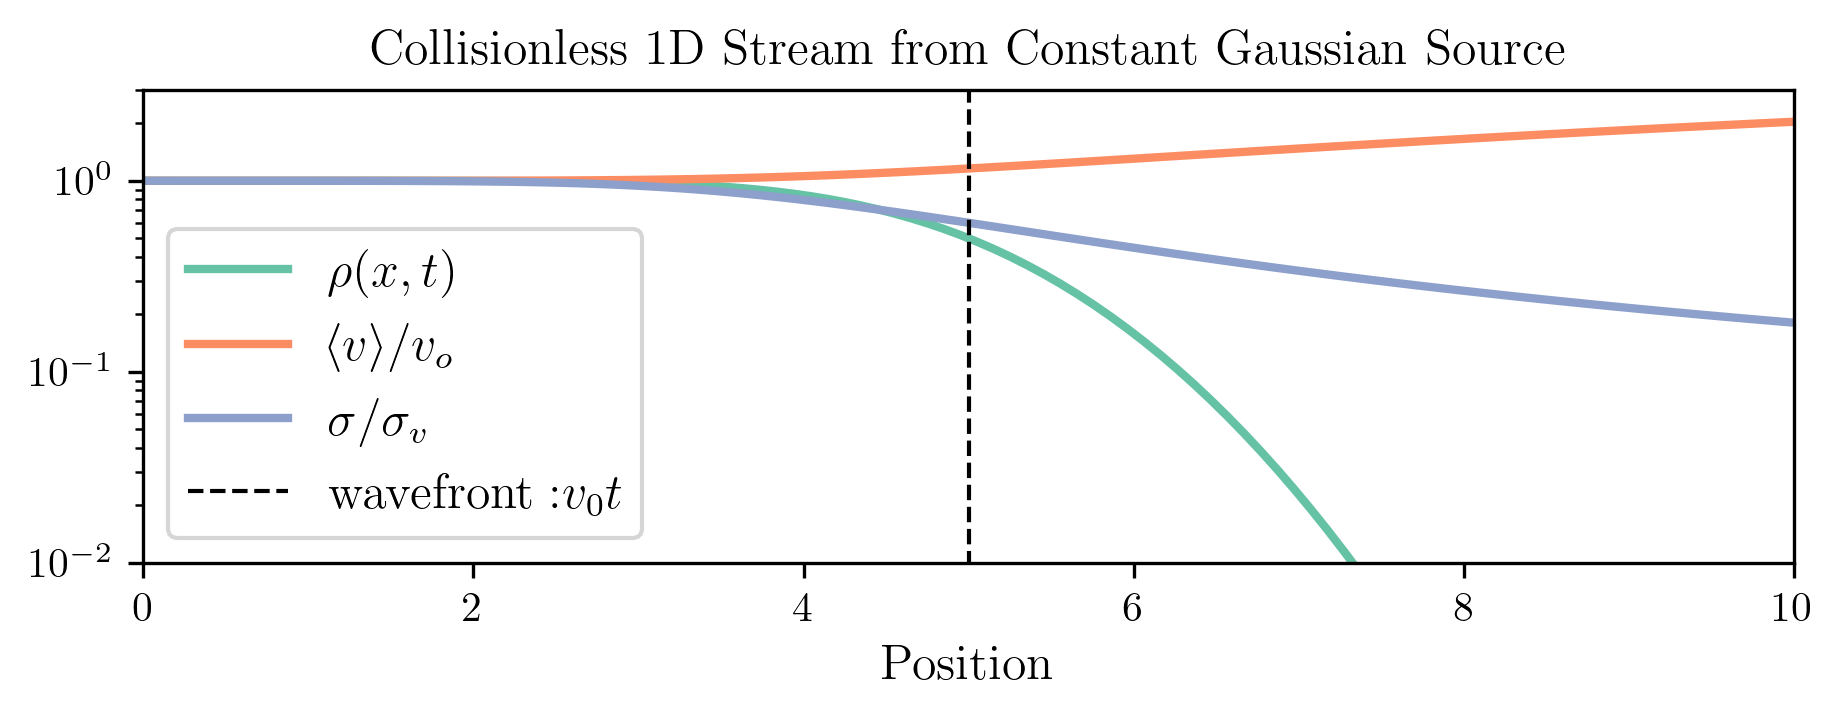
\includegraphics[width=\linewidth]{images/collisionless_1D_stream.png}
                \caption[Moments of dimensional collisionless free streaming from a Gaussian source]{A snapshot at a fixed time of selected moments of the distribution function describing one-dimensional collisionless streaming, used here as an approximation for a stellar stream, as given by Eq.~\ref{eq:one_dimensional_collisionless_streaming}. Particles are continuously injected at the origin with velocities drawn from a Gaussian distribution with mean $v_0$ and dispersion $\sigma_v$. Shown are the particle density, local mean velocity, and local velocity dispersion, all normalized.}
                \label{fig:collisionless_1D_stream}
            \end{figure}

            Understanding the velocity dispersion within the stream is crucial for assessing the formation and persistence of gaps. In Chapter~5, we return to this point in the appendix, where---thanks to a reviewer's suggestion---we analyzed our results by exploring different internal velocity dispersions in the streams, achieved by varying the progenitor's mass. In that chapter, the velocity dispersion is not as simple as in the present case, since particles are released periodically at a rate that scales with the strength of the tidal forces. At each pericenter passage, a large number of particles are ejected, creating conditions even less favorable for gap formation, particularly in regions close to the cluster. We present this analysis in more detail in the Appendix of Chapter~5.

            This section outlined the physics implicit in the equations of motion that underlie our results. Next, we explore some phenomena that were intentionally omitted and discuss how their omission limits the applicability of our findings.
            
\section{The Ignored Physics} \label{sec:ignoredphysics}
    This section could, in principle, be extremely large, since much of physics is irrelevant to our specific problem—neither Schrödinger's equation nor Maxwell's equations are of concern here. But that is not the point. In the previous two sections, I presented our methods and argued for their appropriateness in studying stellar streams originating from Galactic globular clusters. Here, I want to step back and sketch the landscape of what we have chosen to ignore, and highlight other techniques used in the literature. Chief among these is treating the globular cluster as a collisional system.

    I had originally considered discussing additional physical processes, such as a time-varying Milky Way potential or particle-spray methods for modeling globular cluster disruption. However, these are more properly regarded as alternative approaches rather than corrections to our framework. Thus, I limit the discussion here to internal cluster dynamics, and cite two exemplary works that demonstrate how our simulated tidal tails can differ—not only from other models, but potentially from reality itself. For discussion of a time-evolving Galactic potential and particle-spray techniques, see the concluding section on future prospects.
    \subsection{Globular Cluster Internal Dynamics} \label{sec:collisionalDynamics}
        In this thesis, globular clusters are treated primarily as the sources of stellar streams, because our interest lies more in the streams themselves than in the internal structure of the clusters. To that end, we simplified the internal dynamics by assuming a smooth, mean-field potential, fully aware that this is a limiting assumption. We made a deliberate trade: computational efficiency at the cost of dynamical fidelity.

        But how severe is this limitation? By neglecting the collisional nature of globular clusters and adopting a test-particle framework, we constrain our ability to model the rate at which stars escape, the manner of their ejection, and the identity of the stars that escape. Below, I present a basic demonstration of two-body relaxation, followed by a summary of key studies that explore the consequences of including internal cluster dynamics more fully.
        \subsubsection{Two-body Relaxation Time: a derivation and example} \label{sec:twoBodyRelaxation}
            While it is appropriate to treat the orbits of stars in galaxy as collisionless, this approximation breaks down in the context of globular clusters. Here, I present a brief numerical experiment to illustrate the concept of two-body relaxation, which quantifies the breakdown of the mean-field approximation.

            Two-body relaxation asks: how long does it take for the discrete, granular nature of the stellar medium to cause a star's trajectory to deviate significantly from the one it would follow in a perfectly smooth (mean-field) potential? This timescale is defined by the condition: $\delta v / v_0 \sim 1$, meaning that the change in the velocity due to the medium roughly the original speed.

            In this context, we simplify the star's motion, neglecting the complexity of orbital paths in a galaxy. Instead, we consider uniform motion through a medium composed of discrete masses. If the medium consists of many small-mass particles, the potential is smoother and better approximates the mean field. If there are fewer particles with larger mass, each interaction can cause a significant deflection.

            For a single interaction in the impulse approximation, the change in velocity is:
            \begin{equation}
                \delta \mathbf{v} = \frac{Gm}{bv} \begin{bmatrix} 0 \\ \cos\theta \\ \sin\theta \end{bmatrix},
                \label{eq:delta_v_vec_impulse_approx}
            \end{equation}
            where $b$ is the impact parameter, $m$ the perturber's mass, $v$ the relative velocity, and $\theta$ the angle in the transverse plane. These impulses deflect the star sideways but not along the direction of motion — a key assumption in the impulse approximation.

            Now consider not just one fly-by, but a sequence of them. A real galaxy has a radially decreasing density, so a star never sees a symmetric distribution unless it is exactly at the center — but we are interested in fluctuations from the mean field, not the mean field itself. That is, if $\Phi_\mathrm{MW} = \Phi_\mathrm{mean}(\vec{r}) + \Phi_\mathrm{stochastic}(\vec{r})$, we are isolating the stochastic part.

            To simplify further, we idealize the galaxy as a cylinder of radius and length $R$, with uniform number density $n = N_p / (\pi R^3)$. As the star moves through this medium, we apply Eq.~\ref{eq:delta_v_vec_impulse_approx} to compute cumulative velocity kicks. This is demonstrated numerically in Fig.~\ref{fig:twoBodyRelaxation}.
            \begin{figure}
                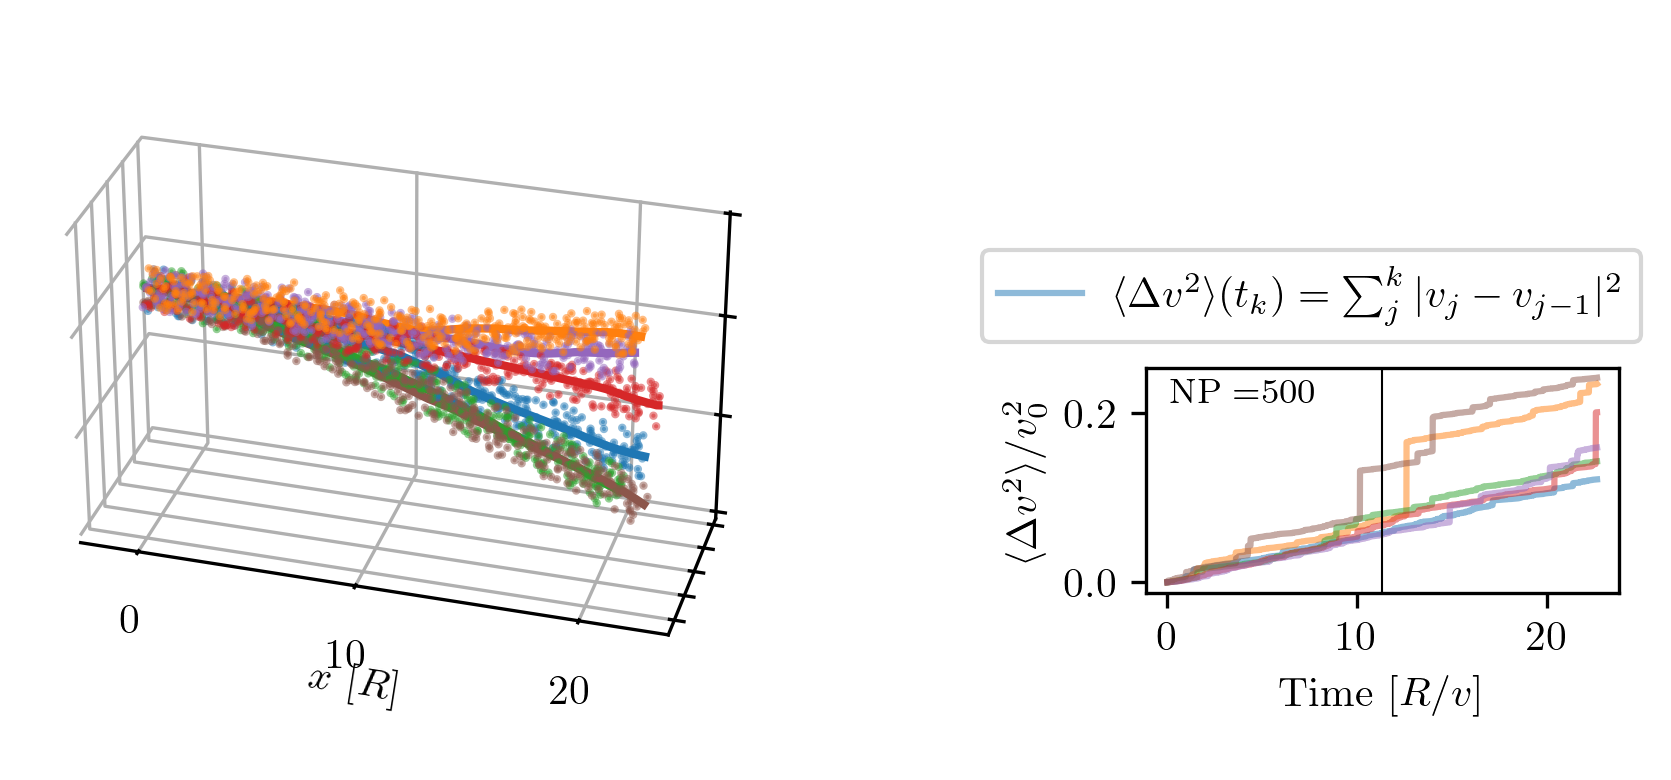
\includegraphics[]{images/twoBodyRelaxation.png}
                \caption[Illustration of two-body relaxation]{Demonstration of two-body relaxation. A star travels through a medium with uniform number density ($n = 500/\pi R^3$). Six independent trajectories are shown, each sampling a different realization of the same underlying number density. Particles are generated on-the-fly as the star moves. The right panel shows the cumulative squared change in velocity. The vertical line indicates the theoretical two-body relaxation time}
                \label{fig:twoBodyRelaxation}
            \end{figure}
            To perform this experiment, I normalize units such that $G = M = R = t_\mathrm{cross} = 1$, giving $v_0 = 1$ and $m = M/N_p$. For Fig.~\ref{fig:twoBodyRelaxation}\footnote{The two-body relaxation experiment is purely illustrative. Despite multiple attempts, I was unable to make the numerical results consistent with the theoretical prediction. Not only is the relaxation process significantly slower than expected, but the discrepancy also worsens with increasing particle number. I rewrote the script several times but was unable to identify the issue. Nonetheless, the main takeaway remains valid: gravitational two-body encounters induce a random walk in velocity space.}, $N_p = 500$, so the number density is $500/\pi$. 

            At each timestep $dt$, a cylindrical volume $\pi R^2 v dt$ is populated with a Poisson-sampled number of particles, where the expected number is $\langle N_{p,\mathrm{disc}} \rangle = n \pi R^2 v dt$. Each particle contributes a velocity kick via Eq.~\ref{eq:delta_v_vec_impulse_approx}, which is summed over time to compute the net velocity and trajectory.

            I would like to present some key steps in the theoretical derivation. In this idealized model, we expect:
            \begin{equation}
                \langle \delta \mathbf{v} \rangle = \mathbf{0},
            \end{equation}
            since the medium is isotropic and random, so kicks cancel on average. However, the mean squared change is non-zero:
            \begin{equation}
                \left\langle \delta v^2 \right\rangle \neq 0.
            \end{equation}
            $\left\langle \delta v^2 \right\rangle$ can be found by reasoning on the number of expected interactions from each shell of a cylinder, where the volume infinitesimal is: $rd\theta dr(vdt)$. We find that this \textit{diffusion} grows linearly with time, and its rate of change gives the two-body relaxation timescale:
            \begin{equation}
                \tau_\mathrm{2-body} = \frac{v_0^2}{\frac{d \left\langle \delta v^2 \right\rangle}{dt}}.
            \end{equation}
            Another key in this derivation is the Coulomb integral, which involves a logarithmic divergence:
            \[
            \int \frac{1}{R} \, dR.
            \]
            We must regularize this with appropriate limits. The upper limit is the system size (no perturbers beyond this). The lower limit corresponds to where the impulse approximation breaks down — I choose the distance at which a star becomes gravitationally bound to the perturber, though this is generous and the impulse approximation breaks down at larger distances.

            The resulting expression for the two-body relaxation time is \citep{2008gady.book.....B}:
            \begin{equation}
                \tau = t_\mathrm{cross} \, \frac{N}{8 \ln(N/2)}.
            \end{equation}
            Let's apply this to globular clusters using their catalog values. Take the median crossing time per star as
            \[
            t_\mathrm{cross} = \sqrt{\frac{r_{1/2}^3}{GM}},
            \]
            assuming an average stellar mass of 0.41 $M_\odot$ \citep{1998A&A...330..480B}. With this, only a handful of clusters have relaxation times greater than the 5 Gyr integration time used in our simulations. In ascending order, these include: \textit{NGC6356, NGC5897, NGC6715, Pal4, AM1, Arp2, NGC5053, Crater, NGC5024, Pal5, NGC6101, IC4499, Pyxis, Pal3, Ter8, Pal15, Pal14, FSR1758, SagittariusII, NGC5139, NGC2419}. Across the catalog, the average relaxation time is 2.8 Gyr, the median is 1.5 Gyr, the maximum is 40 Gyr, and the minimum is 0.07 Gyr.
        
            \subsubsection{Beyond Two-Body Relaxation}
            Our modeling of globular cluster dissolution via the restricted three-body problem neglects internal dynamics such as two-body relaxation, binary interactions, and stellar evolution. While this simplification allows us to isolate the effects of tidal stripping, it limits the generality of our predictions. In particular, internal processes can influence both the rate and nature of stellar escape, affecting the morphology, kinematics, and observability of stellar streams.

            A range of internal mechanisms can eject stars from a cluster independently of tidal forces \citep{2003gmbp.book.....H}, and have been studied for decades \citep{1978RvMP...50..437L,1990ApJ...351..121C,1997A&ARv...8....1M}. For instance, binary stars are common in globular clusters, and given the high stellar densities, interactions with a third body can occur. At the end of such encounters, one of the stars may be ejected with sufficient energy to escape the cluster. This process was studied in detail by \citet{2023MNRAS.518.4249G,2024MNRAS.528.5189G}, who simulated the Milky Way globular cluster system using three-body ejections rather than tidal stripping as the escape mechanism. Their results—one of which is shown in Fig.~\ref{fig:grondin_et_al_core_spray}—produce a much more diffuse distribution of escaping stars than our models. In some cases, the ejection energy is sufficient to overcome the effective potential barrier entirely (see Fig.~\ref{fig:CR3BP_forbidden_region}), allowing stars to escape in any direction. Some may even reach velocities above the Galactic escape speed, potentially contributing to the population of hypervelocity stars observed by Gaia \citep{2021ApJS..252....3L}.
            \begin{figure}
                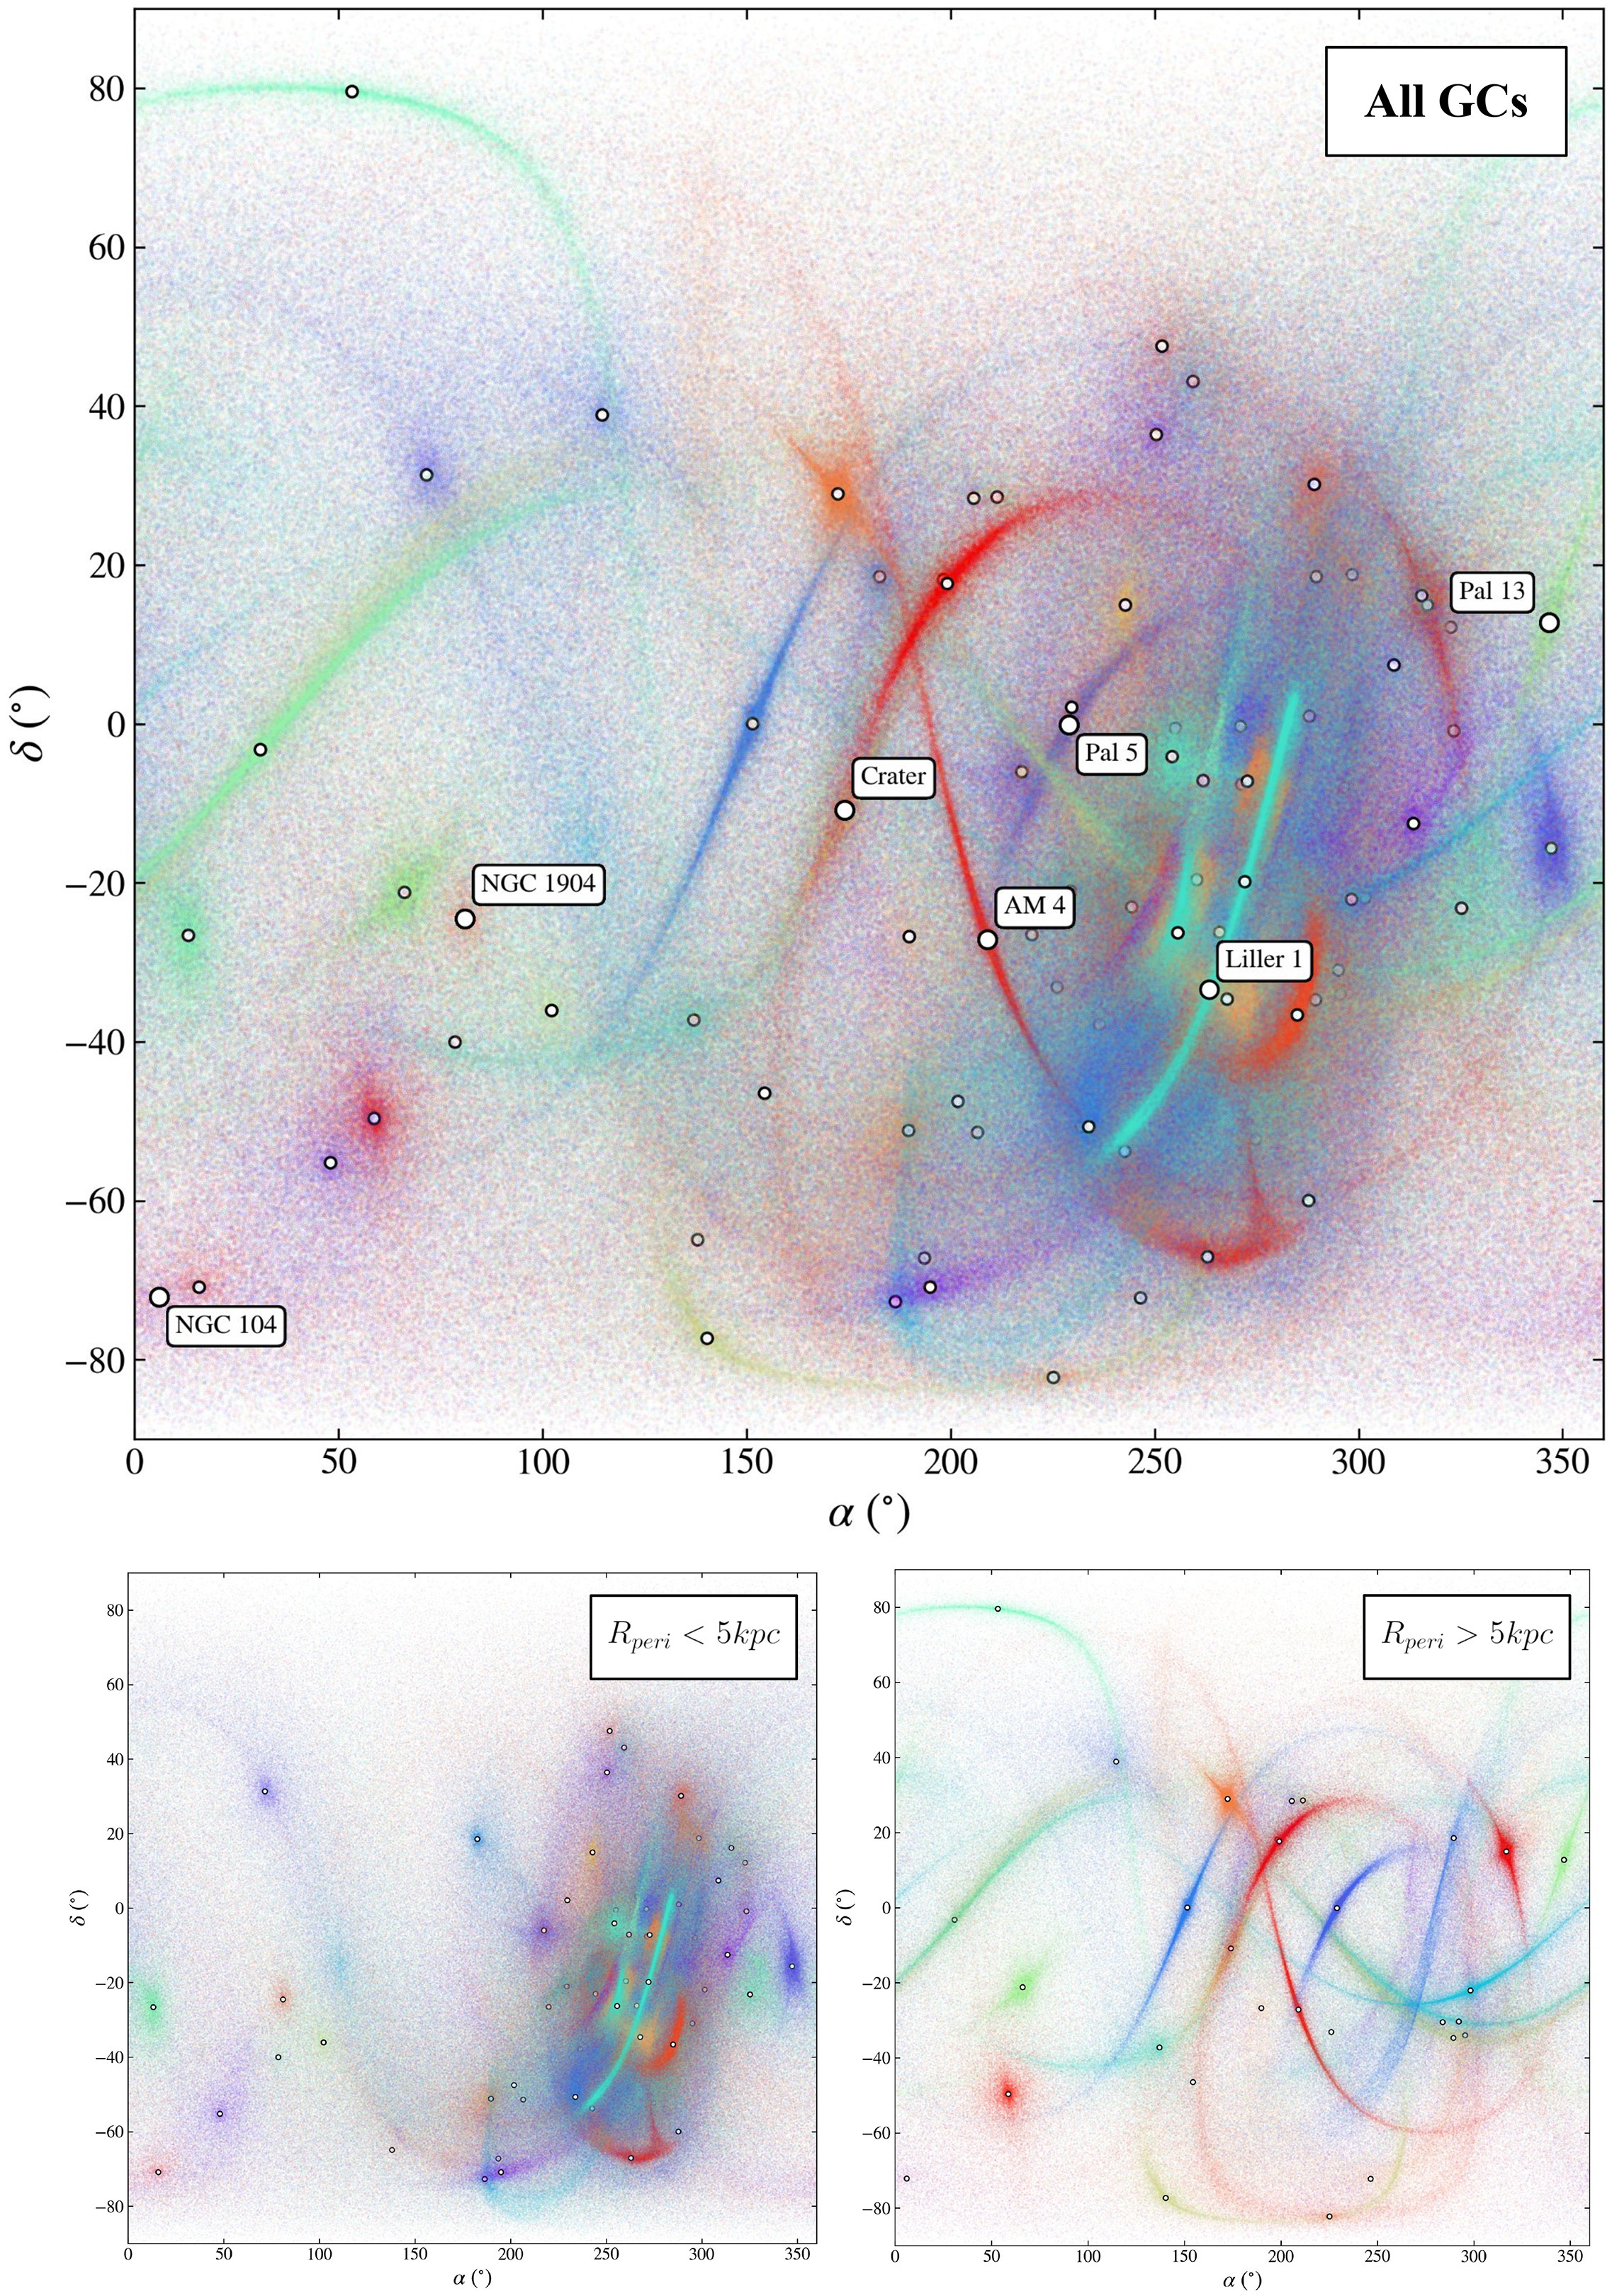
\includegraphics[width=\linewidth]{images/grondin_et_al_core_spray.jpeg}
                \caption[Milky Way Globular Cluster debris ejected from clusters' cores]{Expected distribution of stars from the Milky Way globular clusters that are ejected from globular cluster cores via 3-body interactions. Reproduced from \citet{2024MNRAS.528.5189G}.}
                \label{fig:grondin_et_al_core_spray}
            \end{figure}            
            Incorporating a stellar mass function introduces additional dynamical effects. One of the earliest empirical mass functions was proposed by \citet{1955ApJ...121..161S}, and a widely used modern version is the piecewise form by \citet{2001MNRAS.322..231K}, which accounts for the tapering at the low-mass end. A well-known consequence of having a range of masses is \textit{dynamical friction} \citep{1943ApJ....97..255C,1943ApJ....97..263C,1943ApJ....98...54C}, whereby massive stars lose orbital energy through interactions with lighter stars and sink toward the cluster center. This process leads to \textit{mass segregation}, the tendency for massive stars to concentrate near the core. The statistical trend underlying this is toward energy equipartition, where the average kinetic energy per star is constant. Since $E \propto m \langle v^2 \rangle$, this implies $\langle v^2 \rangle \propto 1/m$. In real clusters, however, the relaxation time can be long, and complete equipartition may never be achieved \citep{2016MNRAS.458.3644B,2025A&A...698A.209Z}. Moreover, tides preferentially remove stars on weakly bound (i.e., high-energy) orbits, which tend to be lower-mass stars—so tidal stripping acts as a mass filter.

            Beyond assigning mass to the stars, we can consider them as actual stars, i.e., luminous, gaseous bodies in hydrostatic equilibrium. Relaxing the point-mass assumption leads to a much richer picture. Stars differ in mass, age, and composition, all of which affect their luminosities and thus their detectability. \citet{2008A&A...490..151K} showed that low-mass stars and remnants like white dwarfs are preferentially ejected from globular clusters, altering the cluster's global luminosity profile. Extending this, \citet{2018MNRAS.474.2479B} explored how internal dynamics shape the escape of stars with different luminosities and found a seemingly paradoxical result: more massive clusters can produce \textit{less detectable} streams. The reasoning is twofold: more massive clusters retain more low-mass stars, which are intrinsically fainter, and these same stars are more likely to be stripped. As a result, even though the streams may be more massive, they are harder to detect (see Fig.~\ref{fig:balbinot-2018}).
            \begin{figure}
                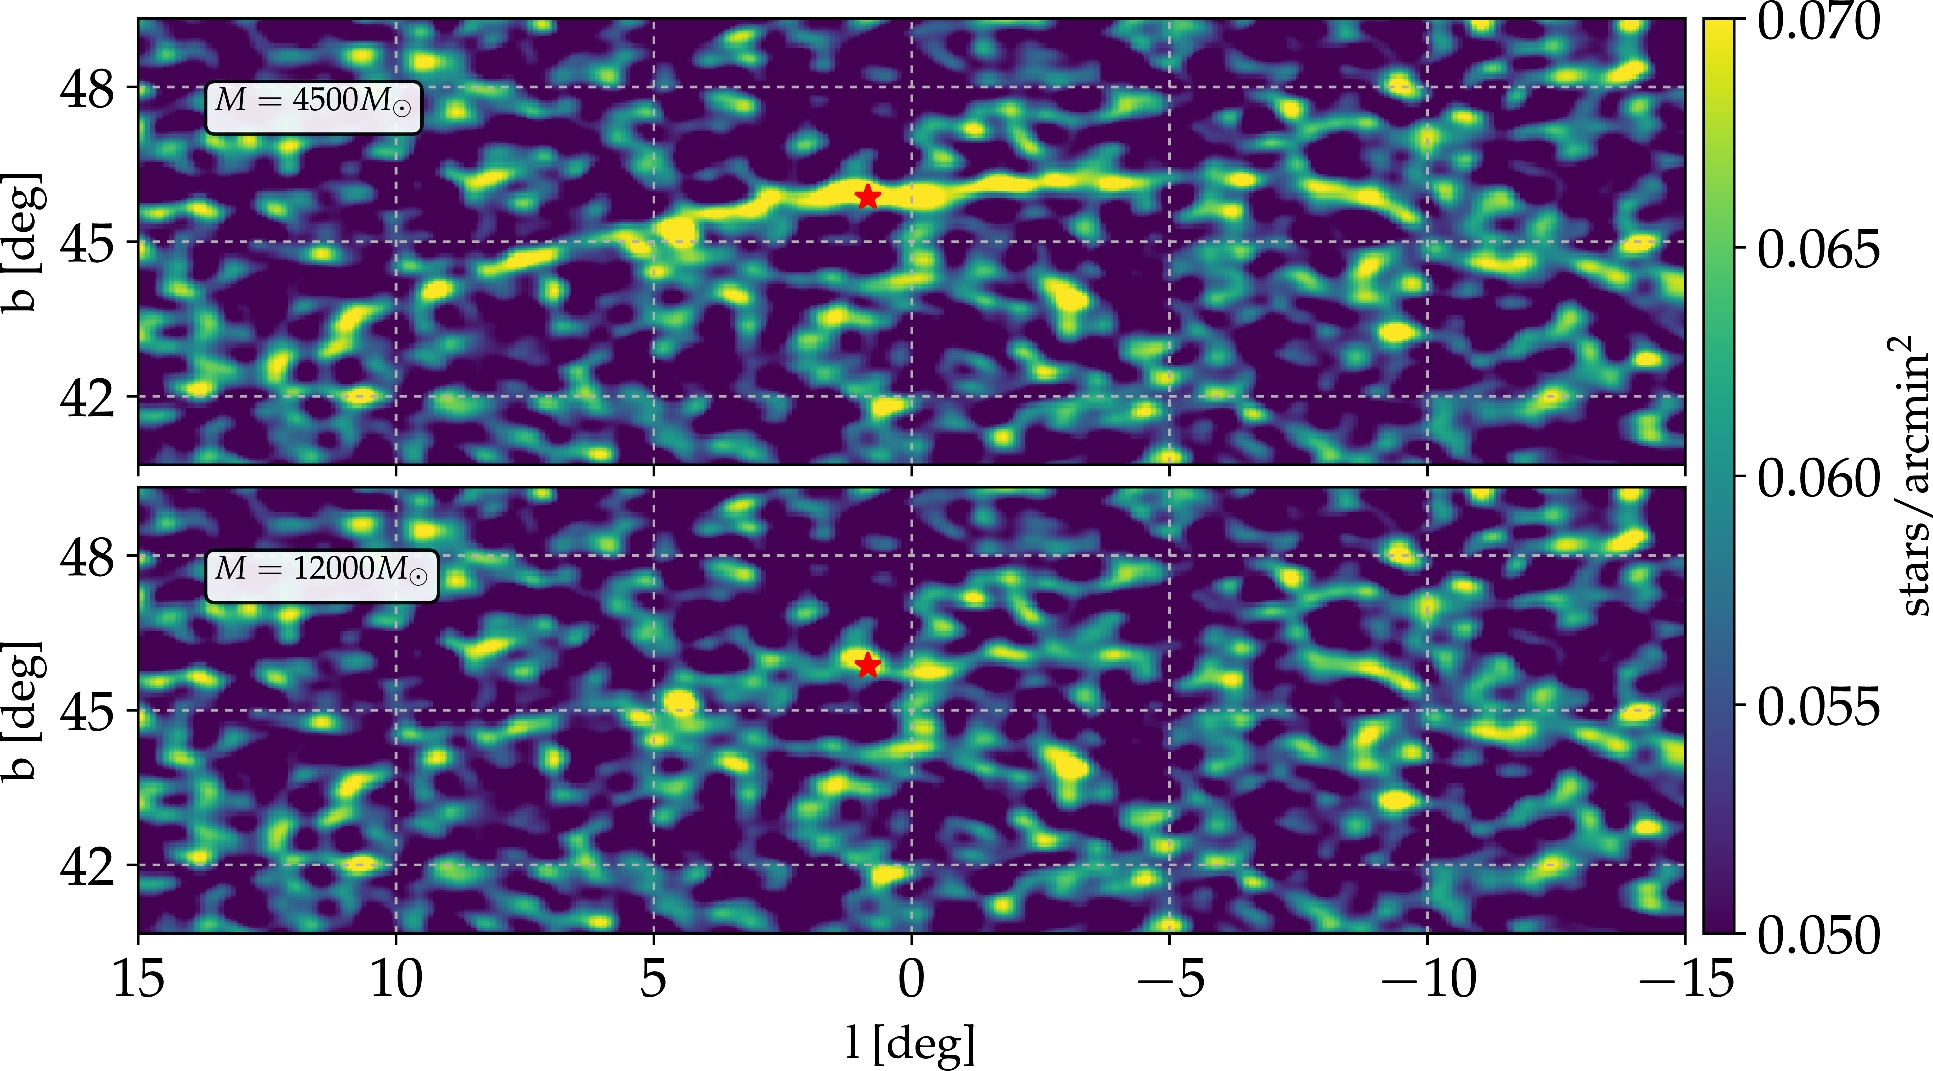
\includegraphics[width=\linewidth]{images/balbinot-2018.jpeg}
                \caption[Effects of mass-segregation on stream observability]{Effects of mass-segregation on stream observability. Two different simulations of Palomar~5, one in which it's mass is artificially increased, which in turn preferentially ejects low-mass dim stars. Reproduced from \citep{2018MNRAS.474.2479B}.}
                \label{fig:balbinot-2018}
            \end{figure}
            Stellar evolution affects not only the stars' luminosities but also the dynamics of the cluster. \citet{2018MNRAS.474.2479B} included stellar evolution in their simulations and showed how mass loss from evolving stars alters the cluster's potential. The most significant phase occurs in the first $\sim$1~Gyr, when massive stars explode as supernovae, ejecting substantial mass and weakening the cluster's potential well. \citet{2010MNRAS.409..305L} decomposed cluster mass loss into three stages, the first of which—driven by stellar evolution—dominates the early lifetime. If an exploding star is part of a binary, its companion may also be ejected. The extent of this effect depends strongly on both the initial mass function and metallicity of the cluster.\footnote{I once wondered whether the kinetic energy deposited by a supernova's ejecta might dynamically affect nearby stars. A quick back-of-the-envelope estimate suggests it is negligible. The mass simply puffs out of the cluster.}
